\documentclass[12pt,a4paper,oneside,english]{report}
\special{papersize=210mm,297mm}
%\usepackage[T1]{fontenc}
%\usepackage[latin1]{inputenc}
\usepackage[cm]{fullpage}
\usepackage[english]{babel}
\usepackage[pdftex]{graphicx}
\usepackage[labelsep=period]{caption}
\usepackage{subcaption}
\usepackage{color}
\usepackage{fixltx2e}
\usepackage{epstopdf}
\usepackage{hyperref}
\usepackage{float}
\usepackage{textcomp}
\usepackage{circuitikz}
%\usepackage{subfig}
\graphicspath{{./FIG}}

\begin{document}
\ctikzset{bipoles/length=.6cm}
\ctikzset{bipoles/thickness=4}
\newcommand\electricC {
\hspace{-14 pt}
\begin{circuitikz}
\draw (0,0) to[capacitor] (0:1);
\end{circuitikz}
\hspace{-6 pt}
}
\newcommand\electricR {
\hspace{-14 pt}
\begin{circuitikz}
\draw (0,0) to[european resistor] (0:1);
\end{circuitikz}
\hspace{-6 pt}
}
\newcommand\electricL {
\hspace{-14 pt}
\begin{circuitikz}
\draw (0,0) 
 to[american inductor] (-1,0) 
;\end{circuitikz}
\hspace{-6 pt}
}
\newcommand\electricDAK {
\begin{circuitikz}
\draw (0,0) to[full diode] (0:1);
\end{circuitikz}
}
\newcommand\electricDKA {
\begin{circuitikz}
\draw (0,0) to[full diode] (180:1);
\end{circuitikz}
}
\title{TransistorTester with AVR microcontroller \\
and a little more\\
Version 1.13k \\
}
\author{Karl-Heinz K\"ubbeler\\
\texttt{kh\_kuebbeler@web.de}}
\date{\today}
\maketitle
\tableofcontents

\section*{����������}
\subsection*{�������� ������}

������ ������������� ����� ��������� ������: �� ������� ���������� �� �������� ����� ��� ������� ���� �� �������. 
���� �� ��� ���� ����������, � � ��� ��� ���� ������� ��� �� ������ �������� ������������ �� ���� ��������, �� ��� 
� �������. �� ���� ������������ �����������, �� �� ������� �� ������, ��� ��� �� �������. ������������ ������ ��������� 
���� ���������� ������� � ����������. ������� ����� ���� N-P-N, P-N-P, N ��� P-��������� MOSFET ������������ � �.�. 
���� Markus F. ����������� � ���, ����� ���������� ������ ������ �� AVR ���������������.
\subsection*{������ ���� ������ ��� ��������}

��� ������ � ����������� ������������ ������� �� Markus F.\cite{Frejek} ��������, ������ ��� � ���� ���� �������� � 
���� ��������������. � ����� �������� ����� � ��������, �� �� ���� ����������������� EEprom ATmega8 � ��������� Windows 
��� ��������� �� ������. ������� � ���� ����������� ����������� �� Markus F. � ������� ��� ��������� �� ������ EEprom 
� Flash ������. ���������� ����������� ����������� ��� ����, ����� ��������� ������ � ������ ������ ���������, � ���� 
��������� ���� �������� ��������� ������� ReadADC �� ������ ��� �� ����������� (\(mV\)). ����������� � \(mV\) ���������� 
��� ������ ������ �������� ����������. ���� ������� ReadADC ���������� �������� ��������������� � \(mV\), � ���� 
��������� �������������� ��� ������� ��������� ��������. ����������� � \(mV\) ����� ��������, ���� ����������� 
���������� 22 ��������� ���, ����� �������� �� 2 � ��������� �� 9. ����� ������� ������������ �������� ��������� 
\begin{math}\frac{1023\cdot22\cdot2}{9} = 5001\end{math},  ��� �������� ������������� ������ ����������� ���������� 
�������� ���������� � \(mV\). ����� ���� ������������� ���� �������, ��� ����������, �� �����������������, 
���������� ��� ����� �������������� ��������� ���������� � ��� ����������, ��� ������� � AVR121 \cite{AVR121}. 
� ������������ ������ ������� ReadADC ������������� ��������� 20 ��������� ��� � ������� ����� �� 20, ��� ��� ��������� 
����� ������������� ���������� ���. �.�., �� ����� ���� ��������� ���������� ��� ����������. ��� ��� � ������ ��� 
������� ��������� ������, ����� �������� ������� ReadADC, � ��� ��������� ���������������� ��� ��������� � �������� ��� 
�if statements�  � ���������, ��� ������������� �������� ����������. �� ��� ���� ������ ������� ���� ������!\\

���������� ��� ������ � ������ ����, ����� ������� ��������� ����� �������� � �������. ����� ���� �������� ��������� 
�������� ��������� ������������� � ��������. ������ ������ ���������� �� LCD-������� ��� �������, ������ ��� ������, 
���������� � ������������� ������������ �������, � �� �����. ��� ��������� �������������� ���������� ���������� 
������������ �� ������� ��������� ������� � ����� \ref{sec:features}. ����������� ������ � ����� ���� ������������ 
� ����� \ref{sec:todo}. ������, ������ � ���� ��������������� EEprom ATmega � ������������ ������� Linux ��� ������.\\

����� � ����� �� ������������� ������������ � ������ ������������ ����������� Markus Frejek, ������� ����������� 
����������� ���������� ������� �� ������. ����� ����, � ����� �� ������� ������� ������� �������������� ���������� 
�� ������, ������� ������� ��� ����� ����� ������, ������ ����� � ������. ����� � ����� �� ������������� Markus 
Reschke, ������� �������� ��� ����������� ��� ����� ������ ������������ ����������� �� ������� SVN. 
����� ����, ��������� ���� � ����������� ������ Markus R. ���� ������������� � ��� ����������� ������ ������������ 
�����������.

����� Wolfgang SCH. ��������� ������� ������ �� ��������� ������� ��� ������� � ������������ ST7565. ������� ������� ���
�� ��������� �������������� 1.10k � ������� ������.

� ������ ������������� ����� Asco B., ������� ���������� ����� �������� ����� ��� ���������� ������� 
���������������. ��������� ������������� � ����� �� ��������� Dirk W., ������� ���������� ������� ������ ���� �������� 
�����. � ���� ������� �� ������� �� ������� ���������� ����� ����� ������ ������������ � ����� ������������ 
������������ �����������. ���������� ������� �� ��������� � � ���������� ��������� ����������� ����������� �� ��� �� 
������. ������� �� �������������� ����������� �� ��������� ������� ������ �������� ��������� 
�Deutscher Amateur Radio Club (DARC)� �� Lennestadt.

�� ����������, ������� Nick L �� �������, �� ��������� ���� ������ ����������� ����, ����������� ��������� ���������� �
��������� ��������� � ������� ������������. 

%\newpage
\chapter{Eigenschaften}
\label{sec:features}
\begin{enumerate}
\item Arbeitet mit Mikrocontrollern vom Typ ATmega8, ATmega168 oder ATmega328. Auch ATmega644 und ATmega1284 oder ATmega1280 und ATmega2560 können verwendet werden.
\item Anzeige der Messergebnisse auf einem 2x16 oder 4x20 Zeichen großen LC-Display.
 Alternativ kann bei Verwendung eines Prozessors mit mindestens 32K Flash Speicher auch ein graphisches Display
 mit 128x64 Pixel und ST7565-, ST7920, ST7108, KS0108 oder SSD1306-Controller benutzt werden.
 Dabei wird anstelle der Standard 4-Bit Parallel-Schnittstelle
 auch entweder eine 4-Wire SPI-Schnittstelle oder ein I\textsuperscript{2}C-Bus benutzt.
 Sogar Farbdisplays mit ILI9163 oder ST7735 Controller sind mit der SPI-Schnittstelle anschliessbar.
 Für den ST7108 oder KS0108 Controller ist ein seriell-parallel Wandler 74HC(T)164 oder 74HC(T)595 erforderlich,
 da diese Controller nur den 8-Bit parallel Anschluß erlauben.
 Displays mit PCF8812 oder PCF8814 Controller können ohne die großen Transistor-Symbole benutzt werden, da
die Displaygröße unzureichend ist (102x65 und 96x65).
\item Ein-Tasten-Bedienung mit automatischer Abschaltfunktion.
\item Batterie-Betrieb ist möglich, weil der Strom im abgeschalteten Zustand nur etwa 20nA beträgt.
Ab Softwareversion 1.05k wird nach Möglichkeit in den Messpausen der Schlafzustand des ATmega zum Stromsparen benutzt, wenn kein Impulsdrehgeber benutzt wird.
\item Preisgünstige Lösung ist möglich ohne Quarz und ohne automatische Abschaltung.
\item Automatische Erkennung von NPN und PNP bipolaren Transistoren, N- und P-Channel MOSFETs, JFETs,
Dioden, Doppeldioden, N- und P-IGBTs, Thyristoren und Triacs.
Für Thyristoren und Triacs müssen die Zünd- und Halteströme für die richtige Erkennung erreicht werden können.
Bei IGBTs muß die Gate Schwellwertspannung unter \(5V\) liegen.
\item Darstellung der Pin-Belegung der erkannten Bauteile.
\item Messung des Stromverstärkungsfaktors und der Basis-Emitter-Schwellspannung für bipolare Transistoren.
\item Darlington-Transistoren können durch die höhere Schwellspannung und durch den hohen Stromverstärkungsfaktor erkannt werden.
\item Automatische Erkennung einer Schutzdiode bei bipolaren Transistoren und bei MOSFETs.
\item Messung der Schwellwert-Spannung, der Gate-Kapazität  und des R\textsubscript{DSon} bei einer Gatespannung von knapp \(5V\) von MOSFETs.
\item Bis zu zwei Widerstände werden gemessen und mit den \mbox{\electricR} Symbolen
und den Widerstands-Werten mit bis zu vier Dezimalstellen in der richtigen Dimension angezeigt.
Alle Symbole werden eingerahmt mit den gefundenen Testpin Nummern des Testers (1-3).
Deshalb können auch Potentiometer gemessen werden. Wenn der Schleifer eines Potentiometers auf eine Endposition
gestellt ist, kann der Tester nicht mehr zwischen mittlerem Anschluss und Endanschluss unterscheiden.
\item Die Auflösung der Widerstandsmessung ist jetzt bis zu \(0,01\Omega\), Werte von bis zu \(50M\Omega\) werden erkannt.
\item Ein Kondensator kann erkannt und gemessen werden. Der wird mit dem Symbol \mbox{\electricC}
und dem Kapazitätswert mit bis zu vier Dezimalstellen in der richtigen Dimension angezeigt.
Der Wert kann zwischen \(25pF\) (bei \(8MHz\) Takt, \(50pF\) bei \(1MHz\) Takt) bis \(100mF\) liegen. Die Auflösung kann bis zu \(1pF\) (bei \(8MHz\) Takt) betragen.
\item Bei Kondensatoren mit einer Kapazität über \(20nF\) wird zusätzlich der äquivalente Serienwiderstand (ESR) des Kondensators
mit einer Auflösung von \(0,01\Omega\) gemessen und mit zwei Dezimalstellen angezeigt.
Diese Fähigkeit steht nur zur Verfügung, wenn der ATmega mindestens 16K Flashspeicher besitzt.
\item Für Kondensatoren mit einem Kapazitätswert über \(5000pF\) kann der Spannungsverlust Vloss nach einem Ladepuls bestimmt werden.
Der Spannungsverlust gibt einen Hinweis auf die Güte des Kondensators.
\item Bis zu zwei Dioden werden mit dem Symbol \mbox{\electricDAK} oder dem Symbol \mbox{\electricDKA}
in der richtigen Reihenfolge angezeigt.
Zusätzlich werden die Schwellspannungen angezeigt.
\item Eine LED wird als Diode erkannt, die Schwellspannung ist viel höher als bei einer normalen Diode.
Doppeldioden werden als zwei Dioden erkannt.
\item Zener-Dioden können erkannt werden, wenn die Zener-Spannung unter \(4,5V\) ist.
Sie werden als zwei Dioden angezeigt, man kann das Bauelement nur mit den Spannungen erkennen.
Die äußeren Testpin-Nummern, welche die Dioden Symbole umgeben, sind in diesem Fall identisch.
Man kann die wirkliche Anode der Diode nur durch diejenige Diode herausfinden, deren Schwellwert-Spannung nahe bei \(700mV\) liegt!
\item Wenn mehr als 3 Dioden erkannt werden, wird die gefundene Anzahl der Dioden zusammen mit der Fehlermeldung angezeigt.
Das kann nur passieren, wenn Dioden an alle drei Test-Pins angeschlossen sind und wenigstens eine eine Zener-Diode ist.
In diesem Fall sollte man nur zwei Test-Pins anschließen und die Messung erneut starten, eine Diode nach der anderen.
\item Der Kapazitätswert einer einzelnen Diode in Sperr-Richtung wird automatisch ermittelt.
Bipolare Transistoren können auch untersucht werden, wenn nur die Basis und entweder Kollektor oder Emitter angeschlossen wird.
Bei ATmega mit mehr als 8k Flash Speicher wird außerdem der Sperrstrom mit einer Auflösung von \(2nA\) gemessen.
Der Wert wird nur ausgegeben, wenn er nicht null ist.
\item Die Anschlüsse einer Gleichrichter-Brücke können mit nur einer Messung herausgefunden werden.
\item Kondensatoren mit Kapazitätswerten von unter \(25pF\) werden normalerweise nicht erkannt, 
aber sie können zusammen mit einer parallel geschalteten Diode oder mit einem parallel geschaltetem Kondensator mit
wenigstens \(25pF\) gemessen werden.
In diesem Fall muss der Kapazitätswert des parallel geschalteten Bauteils vom Messergebnis abgezogen werden.
Bei Prozessoren mit mindestens 32K Flash Speicher wechselt der Tester mit einem Kondensator \textgreater~\(25pF\)
an TP1 und TP3 in eine Kondensator-Meßfunktion, die auch Kapazitäten ab \(1pF\) direkt mißt.
\item Bei Widerständen unter \(2100\Omega\) wird auch eine Induktivitätsmessung durchgeführt, wenn der
ATmega wenigstens 16K Flashspeicher besitzt.
Dabei wird zusätzlich zum Widerstands-Symbol \mbox{\electricR} ein Induktivitäts Symbol \mbox{\electricL} angezeigt.

Der Anzeigebereich ist etwa \(0,01mH\) bis über \(20H\), die Genauigkeit ist allerdings nicht hoch.
Das Ergebnis wird nur bei einem Einzelwiderstand zusammen mit dem Widerstandswert angezeigt.
\item Die Messzeit beträgt ungefähr zwei Sekunden, nur Kapazitätsmessungen und Induktivitätsmessungen können länger dauern.
\item Die Software kann für Messserien mit vorgebbarer Wiederhol-Zahl konfiguriert werden, bevor die automatische Abschaltung ausschaltet.
\item Eingebaute Selbsttest-Funktion inklusive einem optionalen \(50Hz\) Frequenz-Generator um die Genauigkeit der Taktfrequenz
und der Verzögerungszeiten zu überprüfen (nur mit mindestens 16K Flash Speicher).
\item Wählbare Möglichkeit den Nullabgleich für die Kondensatormessung und die Innenwiderstände für die
Portausgänge beim Selbsttest automatisch zu bestimmen (nur mit mindestens 16K Flash Speicher).
Ein externer Kondensator mit einer Kapazität zwischen \(100nF\) und \(20\mu F\) an Pin~1 und Pin~3 ist notwendig, 
um die Offset-Spannung des analogen Komparators zu kompensieren.
Dies kann den Messfehler bei Kapazitätsmessungen bis zu \(40\mu F\) reduzieren.
Mit dem gleichen Kondensator wird eine Korrekturspannung zum Einstellen der richtigen Verstärkung für
die ADC Messung mit der internen \(1,1V\) Referenzspannung berechnet.
\item Anzeige des Kollektor-Emitter-Reststroms \(I_{CE0}\) mit stromloser Basis (\(1\mu A\) Auflösung) und
des Kollektor-Emitter Reststroms \(I_{CES}\) mit der Basis auf Emitter-Potential gehalten (nur bei mindestens 16K Flash).
Diese Werte werden nur angezeigt, wenn sie nicht Null sind (besonders für Germanium-Transistoren).
\item Für ATmega mit mindestens 32K Flash-Speicher wechselt der Tester vom Multifunktionstest zu einem Modus als
Widerstands-Meßgerät, wenn bei der automatischen Bauteile-Erkennung nur ein Widerstand an Test Pin 1 (TP1) und
Test Pin 3 (TP3) erkannt wird. Wenn in der Makefile auch die Induktivitätsmessung beim Widerstandsmeßgerät
mit der Option RMETER\_WITH\_L gewünscht wurde, werden bei der Widerstandsmessung auch Induktivitäten gemessen.
Der Betriebsmodus wird durch {\bf[R]} oder {\bf[RL]} auf der rechten Seite von Zeile 1 des Displays angezeigt.
Genau so wechselt der Tester zu einem Kapazitätsmeßgerät, wenn bei der Bauteile-Untersuchung
eine Kondensator an TP1 und TP3 erkannt wurde. Dieser Betriebsmodus wird durch {\bf[C]} auf der rechten Seite der Zeile 1 angezeigt.
In dieser Betriebsart können Kondensatoren ab \(1pF\) gemessen werden. Lediglich für den automatischen Start der Funktion
braucht man einen Kondensator mit mehr als \(25pF\).
Beide Sonderfunktionen können durch einen Tastendruck wieder beendet werden. Der Tester fährt dann mit der normalen
Meßfunktion fort.
\item Für Prozessoren mit mindestens 32K Flash kann eine Dialogfunktion gewählt werden, 
die weitere Einsatzmöglichkeiten zugänglich machen kann.
Natürlich kann über den Dialog auch zu der Transistortester-Funktion zurückgekehrt werden.
\item Mit Dialogfunktion kann am PD4-Port des ATmega eine Frequenzmessung vorgenommen werden.
Die Auflösung beträgt bei Eingangfrequenzen über \(25kHz\) ein Hertz.
Bei niedrigeren Frequenzen kann die Auflösung bis zu \(0,001mHz\) betragen.
Lesen Sie bitte das Unterkapitel \ref{sec:frequency_counter} auf Seite \pageref{sec:frequency_counter},
wie ein Frequenzsignal angeschlossen werden muß.
\item Mit Dialogfunktion und ohne serielle Ausgabe kann eine externe Spannung bis \(50V\) über einen
10:1 Spannungteiler am PC3 Pin gemessen werden. Bei der PLCC-Version des ATmega328 kann auch einer der beiden
zusätzlichen Pinne für die Spannungsmessung zusammen mit der seriellen Ausgabe benutzt werden.
Wenn die Erweiterung für die Zenerdiodenmessung (DC-DC-Konverter)
eingebaut ist, können in diesen Zweig auch Zenerdioden bei gedrückter Taste getestet werden.
\item Mit Dialogfunktion kann eine Frequenzausgabe auf dem TP2-Pin (PB2-Port des ATmega) erfolgen.
Derzeit können von Frequenzen von \(1Hz\) bis \(2MHz\) eingestellt werden.
\item Mit Dialogfunktion kann eine feste Frequenz mit einstellbarer Pulsweite auf dem TP2-Pin (PB2-Port des ATmega)
ausgegeben werden.
Die Breite kann mit kurzem Tastendruck um \(1\%\) und mit längerem Tastendruck um \(10\%\) erhöht werden.
\item Mit der Dialogfunktion kann eine spezielle Kondensatormessung mit ESR-Messung gestartet werden.
Die Funktion wird bei der Auswahl \mbox{C+ESR@TP1:TP3} genannt.
 Kapazitäten ab etwa \(2\mu F\) bis zu \(50mF\) können meistens wegen der geringen Messspannung von etwa \(300mV\)
 im eingebauten Zustand gemessen werden.
\item Bei Prozessoren mit mindestens 32K Flash-Speicher (Mega328) kann der ADC mit der Sampling-Methode so genutzt werden,
daß Kondensatoren unter 100pF mit einer Auflösung von 0.01pF gemessen werden können. Mit der gleichen Methode können
auch Spulen unter 2mH mit deutlich besserer Auflösung über die Resonanzfrequenz mit einem parallelgeschalteten Kondensator 
bekannter Größe bestimmt werden.

\end{enumerate}

 Bei Einsatz des Testers für die Prüfung von Kondensatoren in einer Schaltung sollte besonders darauf geachtet werden,
 dass die Kondensatoren vor der Messung keine Restladung mehr haben.


Thyristoren und Triacs können nur erkannt werden, wenn der Test-Strom über dem Halte-Strom liegt.
Einige Thyristoren und Triacs brauchen auch einen höheren Zündstrom als dieser Tester liefern kann.
Der verfügbare Teststrom ist nur ungefähr \(6mA\)!
Ebenso können IGBTs nur erkannt werden, wenn eine Spannung von \(5V\) für die Gate-Ansteuerung reicht.
Beachten Sie bitte, dass viele Möglichkeiten nur für Mikrocontroller mit wenigstens 16K Programmspeicher wie ATmega168 zur Verfügung stehen. 
Alle Eigenschaften sind sogar nur für Prozessoren mit wenigstens 32K Programmspeicher wie ATmega328 oder ATmega1284 möglich.

\vspace{1cm}
\textbf{{\Large Achtung:}} Stellen Sie immer sicher, dass {\bf Kondensatoren} vor dem Anschluss an den Tester {\bf entladen} sind!
Der Tester könnte sonst beschädigt werden bevor er eingeschaltet ist.
Es gibt nur wenig Schutzfunktion der ATmega-Anschlüsse.
Besondere Vorsicht ist auch geboten, wenn versucht wird, Bauelemente in einer Schaltung zu messen.
Das Gerät sollte in jedem Fall vorher von der Strom\-ein\-spei\-sung getrennt sein und man sollte sicher sein,
dass {\bf keine Restspannung} im Gerät vorhanden ist.




\chapter{Hardware}

\section{Circuit of the TransistorTester}
\label{sec:hardware}
The circuit of the TransistorTester in figure \ref{fig:ttester} is based on the circuit of
 Markus F. released in Abb.~1 of AVR-Transistortester report \cite{Frejek}.
Changed or moved parts are marked with green color, optional parts are marked with red color.

Some changes are made because the electronical power switch make problems in some implementations.
Therefore the resistor R7 is reduced to \(3.3k\Omega\). The capacitor C2 is reduced to
10~nF and R8 is moved so that the PD6 output does not try to switch the C2 capacitor directly.
 Additional blocking capacitors are added and should be placed
near the power connection of the Atmega and near the Voltage regulator.

Because the PD7 input and PC6 (RESET) are the only pins, where pull up resistors where
needed, one extra \(27k\Omega\) resistor is added to the PD7 (pin~13) input. With this modification
the software can disable all internal pull up resistors of the ATmega.

The additional crystal with its \(22pF\) capacitors are optional added. 
The accuracy of a crystal has the benefit of more stable time measurement for getting the
capacitor values.

New software version can use a voltage scale switch of the ADC. The speed of switching is reduced
by the external capacitor C1 at the AREF (21) pin of the ATmega. To avoid slowing down the
measurement speed more than necessary, the value of this capacitor should be reduced to 1nF.
Removing of the capacitor C1 is also possible.
For adapting the software to the actual circuit take a look to the Makefile options in the
configuring chapter \ref{sec:config} at page~\pageref{sec:config}.

Some different versions of R11 / R12 resistor combinations circulates
in the internet. I~have adapted my software to the original of Markus F. \cite{Frejek} with \(10k\Omega\) and \(3.3k\Omega\).
The voltage ration of the divider can be set with Makefile options.

The additional \(2.5V\) precision voltage reference connected at pin PC4 (ADC4) can be used to
check and calibrate the VCC voltage, but is not required. You can use a LM4040-AIZ2.5 (0.1\%),
a LT1004CZ-2.5 (0.8\%) or a LM336-Z2.5 (0.8\%) as voltage reference.
If you don't install the precision voltage reference and you don't add the relay extension,
you should install a pull up resistor R16 to PC4 with a higher resistance value (\(47k\Omega\)).
This helps the software to detect the missing voltage reference.
A optional ISP connector has been added to easier load new software versions to the tester.

\begin{figure}[H]
\centering

\includegraphics[width=18cm]{../FIG/ttester.eps}
\caption{New circuit of TransistorTester}
\label{fig:ttester}
\end{figure}

The table~\ref{tab:display-con} show the assignment of the port D for different display versions
and the assignment of the additional functions.
For the SPI interface a signal LCD-CE is available at the ATmega port. The controller input CE (Chip Enable) can 
be also connected to GND instead of connecting this input to the ATmega output LCD-CE.

\begin{table}[H]
  \begin{center}
    \begin{tabular}{| c || c | c | c | c | c | c |}
    \hline
           & Character     & ST7565 LCD & ST7920 LCD     & ST7108 LCD  & SSD1306     & additional function \\
      Port & LCD           &   SPI      & serial         & serial      &   I\textsuperscript{2}C      & \\
    \hline
    \hline
    PD0    &  LCD-D4       &  LCD-REST  & LCD-REST       & 595-PCLK        &            & \\
    \hline
    PD1    &  LCD-D5       &  LCD-RS    &                & LCD-CS2     &             & rotary encoder 2 \\
    \hline
    PD2    &  LCD-D6       &  LCD-SCLK  & LCD-B0         & 164-595-CLK &  LCD-SDA    & \\
    \hline
    PD3    &  LCD-D7       &  LCD-SI    &                & LCD-CS1     &             & rotary encoder 1 \\
    \hline
    PD4    &  LCD-RS       &            &                & LCD-RS      &             & frequency counter \\
           &               &            &                & 164-595-SER &             &                \\
    \hline
    PD5    &  LCD-E        & (LCD-CE)   & LCD-EN         & LCD-EN      &   LCD--SCL  & \\
    \hline
    PD7    &  pushbutton   & pushbutton & pushbutton     & pushbutton  & pushbutton  & \\
    \hline
    \end{tabular}
  \end{center}
  \caption{Pin assignments for different displays}
  \label{tab:display-con}
\end{table}


The software can follow to another pin assignment of port D for a simpler connection of the
LCD display. 
The following table \ref{tab:grid-change} shows the modifies assignments for the strip grid layout and
the alternativ connection of a graphical display for the micocontrollers ATmega328.
Also the using of port inputs for additional functions is shown.
With the connections for the graphical display with the strip grid option (STRIP\_GRID\_BOARD=1)
the frequency counter function can not be used, because the port PD4 (T0) is used.
But this connection is used by a chinese version with graphical display. 
In most cases the additional functions like rotary encoder or frequency counter are easier to
build with the board versions for a character display, because the required data signals are
routed to the display connector.



\begin{table}[H]
  \begin{center}
    \begin{tabular}{| c || c | c | c | c | c | c |}
    \hline
           & char. LCD    & ST7565 LCD & ST7565 LCD    & additional function \\
      Port &   =1         &   =1       & STRIP\_GRID   & \\
    \hline
    \hline
    PD0    &  pushbutton  &              &             & \\
    \hline
    PD1    &  LCD-D7      &  LCD-SI      & LCD-A0 (RS) &  rotary encoder 2  \\
    \hline
    PD2    &  LCD-D6      &  LCD-SCLK    & LCD-REST    & \\
    \hline
    PD3    &  LCD-D5      &  LCD-A0 (RS) & LCD-SCLK    & rotary encoder 1 \\
    \hline
    PD4    &  LCD-D4      &  LCD-REST    & LCD-SI      & frequency counter \\
    \hline
    PD5    &  LCD-E       &  (LCD-CE)    &             & \\
    \hline
    PD7    &  LCD-RS      &  pushbutton  & pushbutton  & \\
    \hline
    \end{tabular}
  \end{center}
  \caption{port assignments with option STRIP\_GRID\_BOARD}
  \label{tab:grid-change}
\end{table}

\section {Extensions for the TransistorTester}

\subsection{Protection of the ATmega inputs}

For better protection of the ATmega inputs one of the additional circuits~ \ref{fig:relay_addon} 
can be integrated. The de-energized contacts of the relay protect the ATmega without power.
The contacts will be opened by software only for measurement.
Also with the additional diode protection the chance of the ATmega will be better to survive the connection
of a capacitor with higher residual voltage.
A complete protection is not possible. Therefore capacitors should always be discharged before measuring.

\begin{figure}[H]
  \begin{subfigure}[b]{9cm}
    \centering
    
\includegraphics[width=7cm]{../FIG/relay_addon.eps}
    \caption{with Relay}
  \end{subfigure}
  ~
  \begin{subfigure}[b]{9cm}
    \centering
    
\includegraphics[width=7cm]{../FIG/diode_addon.eps}
    \caption{with Diodes}
  \end{subfigure}
  \caption{Additional protection of the ATmega inputs}
  \label{fig:relay_addon}
\end{figure}

You can get a better protection with a relay with 3 changeover contacts, which is shown in figure~\ref{fig:relay_um_addon}.
The discharge current is limited with the resistors and the ATmega-inputs are disconnected in the protected mode.
But you don't forget, that the tester remains unprotected during the measurement sequence.

\begin{figure}[H]
\centering

\includegraphics[width=18cm]{../FIG/relay_um_addon.eps}
\caption{Improved protection with relay}
\label{fig:relay_um_addon}
\end{figure}

\subsection{Measurement of zener voltage above 4~Volt}

If the serial output of text is not required, the Pin PC3 of the ATmega can be used as analog
input for measuring a external voltage. The voltage can be up to \(50V\) with the optional 10:1 resistor
divider and can be used for measuring the breakdown voltage of a zener diode. 
A current limiting power supply with up to \(50V\) can be switched on with low signal at PD7 pin of the
ATmega to deliver current for testing the break down voltage of a zener diode.
Figure~\ref{fig:zener} shows a suggestion for this expansion.
The tester shows the external voltage as long as you hold the key pressed.
About \(40mA\) more battery current is used by this expansion during key pressing.

\begin{figure}[H]
\centering

\includegraphics[width=12cm]{../FIG/zener_exp.eps}
\caption{Expansion for measuring of break down voltage of Zener diodes}
\label{fig:zener}
\end{figure}

The 10:1 voltage divider can be used with the optional dialog part for the ATmega328 without the 
activated DC-DC converter for the zener diode measurement.
Without the pressed key the voltage converter is not powered. For that the external voltage 
(for example battery voltage) can be measured at the zener diode port.
You can only measure positiv DC voltages up to \(50V\).
You have also to respect the correct polarity.

\subsection{Frequency generator}

With the dialog part of the ATmega you can also select a frequency generator, which supports
currently a selection of frequencies from \(1Hz\) up to \(2MHz\).
The output of the \(5V\) signal is done with a \(680\Omega\) resistor to test port TP2.
You can use the GND signal from the minus pin of the zener diode extension or the test port TP1.
The test port TP3 is connected to GND with a \(680\Omega\) resistor.
Of course you can also connect a driver circuit to the ATmega port PB2 with a separate output
driver circuit and a additional output terminal. But the input of this circuit should not insert a
big capacity load for the ATmega output.

\subsection{Frequency measurement}
\label{sec:frequency_counter}

For using the with the dialog selectable frequency measurement is a little hardware extension
necessary. The input pin PD4 (T0/PCINT20) of the ATmega is used for the frequency measurement.
The same pin is also used for the connection of the LCD. With normal layout, the PD4 pin is connected
to the LCD-RS signal, with the strip grid design it is connected to LCD-D4.
For both signals the PD4 pin can be switched to input as long as no output to the LCD is
required. The LCD respect the input value only, if the LCD-E signal is switched to GND.
For driving the input pin from external clock source at least one serial resistor of \(270\Omega\) should be used.
Better you should use the circuit of figure~\ref{fig:FreqMes} .
The voltage at the PD4 pin (LCD-RS or LCD-D4) should be adjusted to \(2.4V\) without the assembled ATmega
or during frequency measurement of the ATmega, to get the best sensivity for the input frequency signal.
The LCD should always be installed for adjusting, because the pull up resistor of the LCD change the voltage.

\begin{figure}[H]
\centering

\includegraphics[width=7cm]{../FIG/Frequency_addon.eps}
\caption{Extension for measurement of frequency}
\label{fig:FreqMes}
\end{figure}

\subsection{Using of a rotary pulse encoder}

For easier control of the menu function for the ATmega328 you can expand the circuit 
by a rotary pulse encoder with a push button.
The circuit~\ref{fig:RotExt} shows a standard expansion for a normal character LCD.
All signals for the connection of the rotary pulse encoder are available at the plug connector
for the LCD. For this reason the expansion can also be easy upgraded for many existing testers.
In many cases the graphical LCD is assembled on a adapter board with some connection pins
of the character LCD. Also in this cases the upgrade with a rotary encoder is not very difficult to do.

\begin{figure}[H]
\centering

\includegraphics[width=6cm]{../FIG/rotary_extension.eps}
\caption{Expansion with a rotary pulse encoder}
\label{fig:RotExt}
\end{figure}

The figure~\ref{fig:RotEnc} shows the feature of two different rotary pulse encoder.
The version 1 has twice as much indexed positions (detents) per turn as pulses per turn.
The version 2 has the same count of detents as pulses per turn.
The slope of one of the two switch signals is sometimes exactly at the detent of the 
rotary pulse encoder.

\begin{figure}[H]
\centering

\includegraphics[width=14cm]{../FIG/rotary_encoder.eps}
\caption{Feature of two different rotary pulse encoder}
\label{fig:RotEnc}
\end{figure}

The figure~\ref{fig:RotBounce} shows a rotary pulse encoder, which has not only
bouncing contacts, but also has a unstable state of one of the switches at the indexed
position (detent). Every change of the state of the switches is detected by the program
and saved in a cyclic buffer. Therefore the last three states of the switches can be checked
after every status change.
For every cycle of switch states a total of four sequences of state can be defined for every direction of rotation.
If there is only one indexed position (detent) for every cycle of switch states, only
one of the state sequence pair must be monitored (WITH\_ROTARY\_SWITCH=2 or 3) for correct counting.
If there are two indexed positions for every cycle of the switch states, as shown in figure~\ref{fig:RotBounce},
you must monitor two pairs of switch state sequences (WITH\_ROTARY\_SWITCH=1).
You can choise any resolution for the WITH\_ROTARY\_SWITCH for a rotary pulse encoder without
indexed positions. A value of 2 or 3 selects the lowest resolution, 1 selects a middle resolution
and 5 selects the highest resulution.
A oscillation of the selection (counter up, counter down) can be avoided with the type of monitoring,
but sometimes a count can be missed with a bad placement of the indexed position.

\begin{figure}[H]
\centering

\includegraphics[width=14cm]{../FIG/rotary_bouncing.eps}
\caption{A rotary pulse encoder with bouncing switches}
\label{fig:RotBounce}
\end{figure}

In place of the two switches of a rotary switch encoder you can also install two seperate
key buttons for Up and Down movement, if no rotation switch encoder is present or favored.
In this case the option WITH\_ROTARY\_SWITCH must be set to 4 for a correct handling of
the program.

\subsection{Connection of a graphical display}

Many thanks to Wolfgang Sch. for his work to support a chinese version with ST7565 controller.
By now you can also connect a graphical 128x64 pixel LCD with a ST7565 controller.
Because the ST7565 controller is connected with a serial interface, only four signal
lines are required. Two port D pins of the ATmega can be used otherwise.
The ATmega processor should have at least 32k flash memory for the support of a graphical display.
The ST7565 controller works with a operating voltage of \(3.3V\) .
Therefore a additional \(3.3V\) voltage regulator is required.
The data sheet of the ST7565 controller does not allow the direct connection of input pins to
\(5V\) signal level. So the extension of figure \ref{fig:ST7565lcd} uses a additional 74HC4050 CMOS
device for the conversion of the voltage level.
You can try to exchange the four 74HC4050 gates with four resistors of about \(2.7k\Omega\).
With the voltage drop at the resistors you will prevent the increase of the \(3.3V\) controller power voltage 
across the diodes of the controller inputs from the \(5V\) ATmega outputs signals.
You have to try, if the signal form with the resistors can be accepted from the ST7565 controller inputs.
The signal form at the controller inputs will be more simular to the output shape of the ATmega with the 74HC4050 gates in any case.\\

\begin{figure}[H]
\centering

\includegraphics[width=14cm]{../FIG/ST7565lcd.eps}
\caption{Connection of a graphical display with ST7565 controller}
\label{fig:ST7565lcd}
\end{figure}

Normally the ST7565 or SSD1306 controller is connected with a 4-wire SPI interface.
But with the SSD1306 controller you can also use a I\textsuperscript{2}C interface with PD2 as SDA and PD5 as SCL signal.
The SDA and SCL signals must be equipped with pull-up resistors of about \(4.7k\Omega\) to \(3.3V\).
A solution for connecting the OLED display shows the figure  \ref{fig:ssd1306i2c}.
The outputs of the ATmega is only switched to \(0V\) for the I\textsuperscript{2}C signals.
Before connecting the pull-up resistors to \(5V\) you must check, if your display module can tolerate
a \(5V\) signal level. Normally the data inputs of the controller are protected with diodes to \(3.3V\).
You should make sure, that you have loaded a program with the I\textsuperscript{2}C support to the ATmega 
before the Display is connected. If you have loaded a program with another interface, 
the output are also switched to the \(5V\) side.
Because I have determined a influence to the tester results across the VCC connection of a OLED module,
a additional decoupling with a serial resistor of \(68\Omega\) with a additional \(10\mu F\) blocking capacitor
is recommended. Instead of the \(68\Omega\) resistor you can also use a inductor with about \(1mH\).
Without the additional filter my tester has reported collector residual currents with bipolar transistors and a
OLED display.
Also you should check the pin sequence of your OLED module, some moduls have a different location of GND and VCC.
 
\begin{figure}[H]
\centering

\includegraphics[width=14cm]{../FIG/SSD1306_I2C.eps}
\caption{Connection of a graphical OLED display with I\textsuperscript{2}C interface}
\label{fig:ssd1306i2c}
\end{figure}

For connection to the ATmega644 series of processors the pins PB2 to PB5 instead of PD0 to PD3 are used.
The exchange of a text display to a graphical display is possible with a adapter printed board because
all required data signals and power signals are available at the LCD connector.
A little simpler is the connection of a graphical display with a ST7920 controller because
the controller can operate with \(5V\) power voltage.
For that the display should offer 128x64 visible pixels.
The display module with the ST7920 controller can be connected with the 4-bit parallel interface or with a
special serial interface., as shown in figure \ref{fig:ST7920lcd}.
 
\begin{figure}[H]
\centering

\includegraphics[width=14cm]{../FIG/ST7920interface.eps}
\caption{Connection of a display with ST7920 controller}
\label{fig:ST7920lcd}
\end{figure}

For both connection types the software must be configured in a special way.
The Makefile option ''WITH\_LCD\_ST7565 = 7920'' must be set in any case, for the serial
connection type you must set also the option ''CFLAGS += -DLCD\_INTERFACE\_MODE=5''.
The orientation of the presentation can be changed with the options LCD\_ST7565\_H\_FLIP and 
LCD\_ST7565\_V\_FLIP in the same way as with the other graphical displays.

A special case is the connection of displays with a ST7108 controller. Because these displays can only use 
the 8-bit parallel interface, you must use a serial to parallel converter.
The simplest way seems to be the use of a 74HCT164 or a 74HCT595 chip.
A suitable suggestion of a connection circuit shows the figure \ref{fig:ST7108lcd} .

\begin{figure}[H]
  \begin{subfigure}[b]{9cm}
    \centering
    
\includegraphics[width=8cm]{../FIG/ST7108serial164.eps}
    \caption{with 74HCT164}
  \end{subfigure}
  ~
  \begin{subfigure}[b]{9cm}
    \centering
    
\includegraphics[width=8cm]{../FIG/ST7108serial595.eps}
    \caption{with 74HCT595}
  \end{subfigure}
  \caption{Connection of a graphical display with a ST7108 controller}
  \label{fig:ST7108lcd}
\end{figure}

You must check the pin layout of your LCD module, some moduls have different signal sequence.
Some different pin layouts found in data sheets for the ABG128064 series are shown in table~\ref{tab:ST7108types}.

\begin{table}[H]
  \begin{center}
    \begin{tabular}{| c || c | c | c | c |}
    \hline
           & 128064H  &  128064G  & 128064C  & 128064B \\
    Signal &         &          &         &         \\
    \hline
    \hline
  VDD (5V) &   1     &  2       &   4     & 2       \\
    \hline
  VSS (GND) &   2     &  1       &   3     & 1       \\
    \hline
 VO (Drive) &   3     &  3       &  (5)    & 3       \\
    \hline
  DB0-DB3   &   4-7   &  7-10    &   9-12  & 7-10    \\
    \hline
  DB4-DB7   &   8-11  &  11-14   &   13-16 & 11-14   \\
    \hline
  CS1       &   12    &  15      &   1     & 15      \\
  CS2       &   13    &  16      &   2     & 16      \\
    \hline
  Reset     &   14    &  17      &   -     & 17      \\
    \hline
  R/W       &   15    &  5       &   7     & 5       \\
    \hline
  RS        &   16    &  4       &   6     & 4       \\
    \hline
  E         &   17    &  7       &   8     & 6       \\
    \hline
  VEE       &   18    &  18      &   -     & 18      \\
    \hline
  LEDA      &   19    &  19      &   17    & (19)      \\
  LEDK      &   20    &  20      &   18    & -      \\
    \hline
    \end{tabular}
  \end{center}
  \caption{Pin layout of different ST7108 moduls}
  \label{tab:ST7108types}
\end{table}

You can also use a display with a PCF8814 controller, which is usualy used in a Nokia 1100 handy for example.
You must check, which interface of the controller is used in your display module.
The PCF8814 controller can support the SPI-interface with 3 lines and 4 lines,
the I\textsuperscript{2}C-interface and a special 3-line interface, which receice
the data/instruction signal as first serial bit before the 8 data bits.
Because the display support only 96x65 pixels, the big icons for transistors are not
used with this controller. The output is simular to the character display.
As with the most graphical displays this controller also operated with 3.3~Volt.
Therefore a signal conversion for the \(5V\) outputs of the ATmega is required.
For the SPI interface and the 3-line interface you can use the outputs of the ATmega
like ''open collector'' outputs with the Makefile option LCD\_SPI\_OPEN\_COL.
You must use ''Pull-Up'' resistors with this option or you should not set
the option PULLUP\_DISABLE in the Makefile.
Currently only the 3-line interface is tested with the PCF8814 controller.

\begin{table}[H]
  \begin{center}
    \begin{tabular}{| c || c | c | c | c |}
    \hline
           &  PCF8814    & PCF8814        & PCF8814     & additional function \\
      Port &    SPI      & 3-line         &   I\textsuperscript{2}C      & \\
    \hline
    \hline
    PD0    &   LCD-RESet  & LCD-RESset       &            & \\
    \hline
    PD1    &   LCD-D/C   & LCD-SCE        &             & rotary encoder 2 \\
    \hline
    PD2    &   LCD-SCLK  & LCD-SCLK       &  LCD-SDIN   & \\
    \hline
    PD3    &   LCD-SDIN  & LCD-SDIN       &             & rotary encoder 1 \\
    \hline
    PD4    &             &                &             & frequency counter \\
    \hline
    PD5    &             & LCD-EN         &   LCD-SCLK  & \\
    \hline
    \end{tabular}
  \end{center}
  \caption{Pin assignments for different interface types of the PCF8814 controller}
  \label{tab:PCF8814-con}
\end{table}

Some code for supporting a PCF8812 controller with 102x65 pixels is also implemented,
but not yet tested.

\subsection{Connection of a graphical color display}

Some Chinese salesmen offer cheap color display modules with a SPI interface.
The picture \ref{fig:Color_both} shows the backsides of two supported modules with 128x128 pixel
and 128x160 pixel. 
The moduls are very small, so the shown text and symbols are very little.
But the appearance is sharp and clear.

\begin{figure}[H]
\centering
\includegraphics[width=8cm]{../PNG/Color_ILI9163_ST7735.jpg}
\caption{Back side of two Color-LCD's}
\label{fig:Color_both}
\end{figure}

The 128x128 pixel modul uses a ILI9163 controller.
The 128x160 pixel modul uses a very simular ST7735 controller.
The modules are tested with a adapter board, which connects the
SPI signals and the power to the terminal for the normal character display.
The adaption of the \(5V\) output signals of the ATmega to the \(3.3V\) inputs of the controller
is ensured with serial \(10k\Omega\) resistors.
The background light (LED) is required for this modules because nothing is readable without it.
Because of the high count of pixels in vertical direction you can display more text lines for this modules.
For the 128x128 pixel display you can display 8 lines of text with a 12x8 font,
for the 128x160 pixel display you can evel show 10 lines of text.
At the picture \ref{fig:Color_PNP} you can see the result of the measurement of a Germanium transistor
at a 128x128 pixel display.

\begin{figure}[H]
\centering
\includegraphics[width=8cm]{../PNG/Color_PNP_ILI9163.jpg}
\caption{Measurement of a bipolar PNP transistors}
\label{fig:Color_PNP}
\end{figure}

The color feature of the modules is currently not used.
Simply the background color and the foreground color can be changed in the file lcd\_defines.h or
in the Makefile.
The 16-bit color model of the controller is used by the software, the foreground color can be changed
with the constant LCD\_FG\_COLOR and the background color with the constant LCD\_BG\_COLOR .


\section{Hints for building the TransistorTester}
Every LCD-display with at least 2x16 character and a HD44780 compatible controller
can be used with the TransistorTester. You should respect the current needed for
illumination, some LCD need lower current than others.
I had tried OLED type displays, but this type cause interference with measurements
of the ATmega and are {\bf not} recommended. Also loading of special characters
for displaying the resistor symbol has caused problems with the OLED.

The resistors R1 to R6 are critical for measurements and this \(680\Omega\) and
\(470k\Omega\) resistors should be measurement type resistors (tolerance of 0.1\%) to
get the full accuracy.
You should use a precision socket for the ATmega microcontroller to enable
the replacement of the microcontroller.
The microcontroller ATmega8, ATmega168 and ATmega328 can be used.
Recommended is a ATmega328, if you wish to use all features.

Anyway you should assemble all parts to printed board without the microcontroller.
A up-to-date low voltage drop regulator like MCP1702-5002 is recommended as IC2, because it
need only \(2\mu A\) of standby current and can still deliver \(5V\), if your input
voltage is only \(5.4V\). But this part is not pin compatible to well known 78L05 with TO92 body!

After checking, that all needed parts are at the correct place, you should
first connect the battery or power supply to the printed board without LCD-display
and microcontroller. You should check the voltage at the power pins of the
microcontroller and LCD-display terminal during the Test key is pressed.
The voltage should disappear, if you release the Test key.
If the voltage had correct polarity and value,
you should disconnect the power and assemble the microcontroller with correct
alignment. Be careful and make sure, that all pins of the microcontroller
are in the socket holes.
Now you can also connect the LCD. Check if power pins of the LCD has the right connection to
GND and VCC of your board.

If you are sure that everything is all right, reconnect the power. 
If you have already programmed the ATmega, you can press the Test button.
By pressing the Test key, the background light of the LCD should switch on.
If you release the Test button, the LED should illuminate weak.
Notice, that the software for the microcontroller must be compiled for the
correct processor type. A program for the ATmega8 does not run on a ATmega168!

\section{Changeover for tester versions designed by Markus F.}
\label{sec:change_markus}
\begin{description}

\item[Voltage control]
If the problem exist, the tester will shut down immediately with every switch on.
With imy suggested setting of the fuses (Makefile) the voltage control of the different
ATmega versions is switched to \(4V\) (brown out level).
This may be the reason why the tester makes trouble with the power on sequence.
The Pin PD6 tries to switch the 100nF capacitor C2 to VCC level causing a voltage
breakdown of the VCC voltage (\(5V\)).
The capacitor C2 can be reduced to \textless~\(10nF\) without problems.
If possible, the direct connection of PD6 should be replaced by a resistor \textgreater~\(220\Omega\).
\item[Improvement of power on circuit]
Often this problem is the reason, if the tester starts with the button hold pressed, but switch off
directly by releasing. The problem is enforced by a high current background light for the LCD.
The resistor R7 to the base of the PNP transistor T3 was optimized with the value \(27k\Omega\) 
too much to save power consuming.
To improve the switching with lower battery voltage or lower current amplification factor of
the PNP transistor T3, you should reduce the resistance to \(3.3k\Omega\).
\item[Additional pull-up resistor at PD7]
The missing pull-up resistor results to a switch off of the tester with the message ''Timeout''
after a short display time.
The software is configured with the option PULLUP\_DISABLE, that all internal pull-up
resistors are switched off. For that reason the voltage of pin PD7 is not definded,
if the level is not switched by the push button or transistor T2 to GND.
One external pull-up resistor of \(27k\Omega\) to VCC avoid this error.
\item[Capacitor C1 at the AREF pin]
Many designs use a \(100nF\) capacitor at the AREF pin, like the design of Markus F. too.
As long as the reference voltage of the ADC is never changed, this is a good solution.
The software of the TransistorTester for the ATmega168/328 uses a automatic selection
of the internal \(1.1V\) reference voltage of the ADC, if the input voltage is below \(1V\).
With this solution a better resolution of the ADC can be reached for little input voltages.
Unfortunately the switching from \(5V\) to \(1.1V\) reference is very slowly. A additional
wait time of \(10ms\) must be respected for this reason.
With changing the capacity value to \(1nF\) this wait time can be reduced significant.
I have not noticed any degration of measurement quality with this change.
Even a removing of the capacitor has no significant change of measurement results.
If you prefer to leve the capacitor unchanged, you can remove the option NO\_AREF\_CAP
in the Makefile to activate longer wait times in the program.
\item[Expanding of a \(8MHz\) crystal]
With some skill you can expand a \(8MHz\) crystal to the backside of the printed board
directly to the pins PB6 and PB7 (pin 9 and pin 10).
My own expansion was done without the both \(22pF\) capacitors.
This solution has operated well with all tested ATmega.
But it is not required to use a crystal. You can still use the \(8MHz\) RC oszillator
by setting the fuses to get the better resolution of time constant for measuring  the capacity values.
\item[Smoothing of the operating voltage]
The original circuit of Markus F. shows only one \(100nF\) capacitor to block the VCC voltage.
This is clearly too little smoothing. You should at least use one \(100nF\) near the ATmega power pins
and one near the voltage regulator. The input of the voltage regulator should be
blocked with a \(100nF\) too.
Additional \(10\mu F\) capacitors (electrolytic or ceramic) at the input and
output of the voltage regulator can stable the voltage level.
Ceramic \(10\mu F\) capacitos with SMD mounting form are easier to use for backfitting
and have usually a lower ESR value. 
\item[Selection of the ATmega processor]
The using of the base function of the tester is still possible with a ATmega8.
The flash memory of that device is used near \(100\%\).
Because the ATmega168 or ATmeg328 processors are pin-compatible to the ATmega8,
I can recommend the replacement.
Actually the price for ATmega328 is so cheap, that there is no reason to take
a ATmega168 type.
With a ATmega168/328 you get the following advantages:
Self test with automatic calibration.\\
Improvement of measurement quality by automatic switching of ADC scale.\\
Measurement of inductors with resistance  below \(2100\Omega\).\\
Measurement of ESR value of capacitors with value of above  \(90nF\).\\
The resolution of resistor measurement below \(10\Omega\) is \(0.01\Omega\).\\
Using of pin PC4 as serial output.\\
\item[Missing precision voltage reference]
Usually the software should detect the missing voltage reference with the unconnected pin PC4.
In this case no VCC=x.xV message should appear in row 2 of the LCD on power on.
If this message appear without the reference, you should connect a \(2.2k\Omega\) resistor
to the PC4 input and VCC.


\end{description}

\section{Chinese clones with text display}
As I know, the tester is rebuild in China in two versions with character displays.
The first model is rebuild from the first design of Markus F. without the ISP port.
The assembled ATmega8 is placed in a socket, so you can replace it with a ATmega168 or ATmega328.
For this version you should consider all the hints of section \ref{sec:change_markus}.
Additional \(100nF\) ceramic cpacitors should be connected near by the VCC-GND and AVCC-GND pins of
the ATmega for better stabilization of the power voltage.
Because there is no ISP connector at the board, you must expand the board with a ISP connector or you
must plug the ATmega to a external socket for programming.
In addition you should notice, that if your ATmega should run with a \(8MHz\) crystal,
your external ISP programmer must have a external clock for programming or a crystal mounted at the socket.\\

The second version of rebuilded tester is build with SMD components. Also the fix installed ATmega168
is a SMD type with 32TQFP body.
Fortunately on the board is a 10-pole ISP connector provided for the programming.
I have analysed the board version ''2.1 2012/11/06''. One error is the assembly of the part ''D1'',
which should be a precision \(2.5V\) voltage reference. Assembled is only a zener diode.
This part should be removed. You can mount a LM4040AIZ2.5 or LT1004CZ-2.5 precision voltage reference
at this place. A missing voltage reference is noticed by the software, so that you must not install
the voltage reference.
My exemplar was delivered with software version 1.02k. The 10-pole ISP plug was not assembled and I must
install a jumper from ISP pin 6 to ISP pin 10. My programmer expect a GND connection at pin 10, but the
board has GND level only on pin 4 and pin 6 of the ISP.
The label of the ATmega168 was rub away and there was no documentation delivered with the part.
The lock fuses of the ATmega were set, so no readout was possible.
But I could install the software version 1.05k without any problems.
Another user has problems with the same software version 1.05k. This user has the chinese board ''2.2 2012/11/26''.
The software runs only without problems, if a additional \(100nF\) keramic capacitor was placed between
the pin 18-AVCC and 21-GND near by the ATmega.
The software 1.05k uses the sleep state of the ATmega for waiting time. For this reason the current alternates
often and the voltage regulator is stressed more.
Further I have noticed, that the VCC voltage is blocked with a \(100nF\) ceramic capacitor and with a
\(220\mu F\) electrolytic capacitor nearby the 78L05 voltage regulator.
The \(9V\) supply voltage is blocked with the same capacitors, but not at the input of the regulator but
at the emitter of the PNP transistor (parallel with the battery). 
The printed circuit board track from the ATmega168 to the test port is very thin, so that a resistance
of \(100m\Omega\) could be measured for one path. This will be the reason for measuring a resistance
of \(0.3\Omega\) for two direct connected pins.
The ESR measuring can usually consider this by zero compensation.
Beginning with version 1.07k  the software does respect this offset for measuring resistors below \(10\Omega\) too.

\section{Chinese clones with graphical display}
Newer rebuilds of the tester like a version from Fish8840  use a 128x64 pixel graphical display.
This version use a modified circuit for the switch on logic. 
The figure \ref{fig:Fish8840} shows a part of the modified circuit.

\begin{figure}[H]
\centering

\includegraphics[width=12cm]{../FIG/Fish8840.eps}
\caption{Part of the circuit from the Fish8840 version}
\label{fig:Fish8840}
\end{figure}

How you can see at the values of resistor R8 and R15,
a 2:1 scaling factor for the battery voltage measurement is used instead of the original scaling factor.
In addition R15 is direct connected to the battery, what results to a power consumption in the switch off state.
The R15 should better be connected to the drain of Q1 or the input of the voltage regulator to prevent this
unneeded battery power consumption.
A suitable change of the printed board is shown in picture \ref{fig:Fish8840patch}.
A circuit path is cut between R17 and D5 and a new conductive path is inserted between Q1 and
R15 with a enameled copper wire.

\begin{figure}[H]
\centering
\includegraphics[width=12cm]{../PNG/Fish8840patch.jpg}
\caption{Picture of the changed Fish8840 printed board}
\label{fig:Fish8840patch}
\end{figure}

The scaling factor of the battery voltage must be specified in any case in the Makefile before any
attempt can be done to replace the original software (BAT\_NUMERATOR=66 for example).

The display module of the Fish8840 tester is equipped with a \(3.3V\) voltage regulator to adapt
the operating voltage of the display controller.
Because the \(3.3V\) operating voltage can be increased with the \(5V\) signal level of the data signals
from the ATmega, a adapter circuit according to the picture \ref{fig:Fish8840Adapt} is recommended.
The four data signal lines are equipped with four serial \(2.7k\Omega\) resistors at a little
breadboard.
Longer spacer bolts must be used to mount the display with the adapter board to the printed board
of the Fish8840 tester now.

\begin{figure}[H]
  \begin{subfigure}[b]{9cm}
    \centering
    \includegraphics[width=9cm]{../PNG/Fish8840Adapt1.jpg}
    \caption{Display with the breadboard adapter}
  \end{subfigure}
  ~
  \begin{subfigure}[b]{9cm}
    \centering
    \includegraphics[width=9cm]{../PNG/Fish8840Adapt2.jpg}
    \caption{Ready mounted Tester}
  \end{subfigure}
  \caption{Adapter for a correctly display connection}
  \label{fig:Fish8840Adapt}
\end{figure}

Instead of this modification you can also use a special output mode of the 4~SPI signals of the ATmega
with the Makefile option LCD\_SPI\_OPEN\_COL .
With this option the outputs are not switched to VCC level,
but the internal ''pull-up'' resistors are switched on during the output of a high level.
If the option PULLUP\_DISABLE is set, additionally a external pull-up resistor for
the ''Reset'' signal (PD0) is required.
Because the data signals are never switched to VCC directly, the \(3.3V\) power of the LCD controller
can not be elevated.
My version of the Fish8840 tester has all signals for connecting a character display
routed to the LCD plug connector.
Therefore you can prepare the board for connection of a character display, if the
female header is completed and the potentiometer for the contrast level is added.
However the supply pin 15 for the background light is connected directly to the VCC level.
If you install a character display, you should check, that your display module
is equipped with a serial resistor for the background LED.
Of course iyou have to adapt the software for different displays. 
Also the hardware extension are possible with the Fish8840 board.\\

All attempt to replace the original software is allways done at one's own risk.
No guaranty can be given for operational capability of newer software versions.
Unfortunately the original state of the chinese software can not be saved because the 
security bits of the ATmega328 are set. So there is no way to get back to the original state.\\


A additional version with graphical display is the WEI\_M8 printed board, which is shown in picture~\ref{fig:WeiM8}.
This build use a LiIon accumulator with AA (mignon) size as power supply, which can be loaded
with the micro USB plug. Operating is also possible without the accumulator, only with the USB power.

\begin{figure}[H]
\centering
\includegraphics[width=12cm]{../PNG/WEI_M8.JPG}
\caption{Picture of the chinese WEI\_M8 tester}
\label{fig:WeiM8}
\end{figure}

It is pleasant, that the signal lines of the display are equipped with serial resistors
at the adapter board, as you can see in the left picture of~\ref{fig:WeiM8int}.
Therefore you must not be afraid that the \(5V\) signals of the ATmega can cause a excessive
increase of the \(3.3V\) power of the display controller.

\begin{figure}[H]
  \begin{subfigure}[b]{9cm}
    \centering
    \includegraphics[width=9cm]{../PNG/WEI_M8_D.JPG}
    \caption{Adapter board for the display}
  \end{subfigure}
  ~
  \begin{subfigure}[b]{9cm}
    \centering
    \includegraphics[width=9cm]{../PNG/WEI_M8_L.JPG}
    \caption{Base board}
  \end{subfigure}
  \caption{Inside look to the WEI\_M8 Testers}
  \label{fig:WeiM8int}
\end{figure}

With the upgrade to version 1.12k some problems has occured.
If the extended fuse is set to 0x04 (0xfc) as recommended, some measurements has
caused a ''Brown Out'' reset of the processor.
This resets are caused by short voltage drops of the VCC power.
I have added a additional \(4.7\mu F\) ceramic capacitor at the input side of
the voltage regulator and a \(10\mu F\) ceramic capacitor at the output side (VCC)
of the regulator.
Both before and after the upgrade I have noticed, that with bipolar transistors
a residual collector current (ICEO or ICEs) of about \(1\mu A\) was detected with this board.
Not until the unknown LDO voltage regulator was replaced with a MCP1702-5002 this
effect has disappeared. The figure \ref{fig:WeiM8mod} shows the modified board with
the slantwise mounted capacitors and the MCP1702 regulator.
If you don't wont to modify your board, you must set the extended fuse to 0x07 (0xff)
to enable a regular operation. With that setting the voltage drops remain undetected.

\begin{figure}[H]
\centering
\includegraphics[width=12cm]{../PNG/WEI_M8_modified.JPG}
\caption{Picture of the modified WEI\_M8 Tester}
\label{fig:WeiM8mod}
\end{figure}

A additional chinese version with graphical display is the ''LCD-T4'' tester with a yellow 
printed board.
I have removed the display for replacing the software with a newer version.
At the right picture of figure~\ref{fig:T4_front} you can see in the right upper corner the ISP male connector
with correct orientation beside the six holes of the board.
For programming the ATmega I have not soldered the male connectorr. I have only pugged it into
the holes instead and have fixed it with a finger during the programming.
With that procedure the male connector can be easy removed an the display can be mounted again to
it's origin place.
The chinese software could be replaced with the 1.12k without any noticeable problem. 
Also the activating of the ''brown-out'' monitor by setting the extended fuse has not
shown any surprice.

\begin{figure}[H]
  \begin{subfigure}[b]{9cm}
    \centering
    \includegraphics[width=9cm]{../PNG/T4_front.JPG}
    \caption{completely}
  \end{subfigure}
  ~
  \begin{subfigure}[b]{9cm}
    \centering
    \includegraphics[width=9cm]{../PNG/T4_front_noLCD.JPG}
    \caption{with removed display}
  \end{subfigure}
  \caption{Front view of the T4 tester}
  \label{fig:T4_front}
\end{figure}

You can see the upgraded \(5mm\) threaded bolt and the upgraded cables with measurement clips
at the pictures of the back side in figure \ref{fig:T4_back}.
Because the data signals for the graphical LCD controller have also no
level adaption (\(5V\) -\textgreater~\(3.3V\)), the setting of the option LCD\_SPI\_OPEN\_COL is recommended.
Due to the fact, that the board can not be easy upgraded with a ''pull-up'' resistor,
it make sense to remove the option PULLUP\_DISABLE instead. 
This board is lesser practical for later extensions, a replacement of the display is
also difficult to realize.

\begin{figure}[H]
  \begin{subfigure}[b]{9cm}
    \centering
    \includegraphics[width=9cm]{../PNG/T4_back.JPG}
    \caption{components side}
  \end{subfigure}
  ~
  \begin{subfigure}[b]{9cm}
    \centering
    \includegraphics[width=9cm]{../PNG/T4_back_clips.JPG}
    \caption{with measurement cables}
  \end{subfigure}
  \caption{Back side of the T4 tester}
  \label{fig:T4_back}
\end{figure}

A additional chinese version with graphical display is offered with the name ''GM328''.
For this version the graphical display is connected with a adapter circuit board to the 16-pol female connector. 
The port PD5 of the ATmega is connected via pin 6 of the female connector to the CE (Chip Enable) input of the 
graphical controller.
The signal CE is also conneted at the adapter board to the \(0V\) power (GND).
This will resulte to a short-circuit if the ATmega will switch the PD5 output to \(5V\).
But newer versions of the software also switch the CE signal, even if the signal is not necessary for
correct operation.
For correct operation of the ''GM328'' tester with newer software versions you should cut the
connection of the CE signal to pin 6 of the male connector.

\section{Chinese kits with graphic displays}

Two different kit versions with graphical display and rotary encoder are known until now.
The first released kit use a display with a ST7565 or compatible controller (128x64 pixels).
In addition to the rotary encoder a additional input for frequency measurement is provided.
For the test ports a 14-pin Textool socket, three soldering pads for cables and a testpad
for SMD parts are provided at the main board.
The pictures~\ref{fig:Kit_mono} shows the mounted kid.
One of the both \(22 pF\) capacitors was replaced with a trimmer at the soldering side.
With a trimmer the frequency of the crystal can be adjusted for better accuracy of frequency measurement
and frequency generation. 

\begin{figure}[H]
  \begin{subfigure}[b]{9cm}
    \centering
    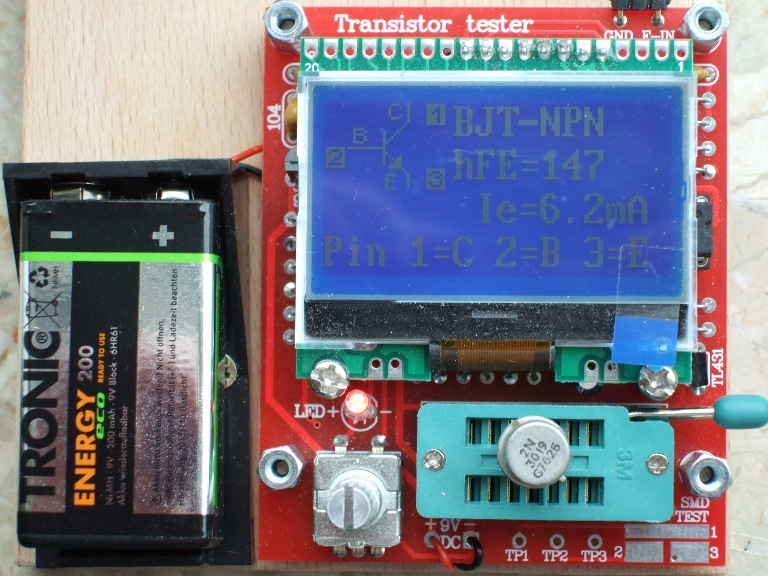
\includegraphics[width=9cm]{../PNG/Kit_ST7565a.jpg}
    \caption{build together}
  \end{subfigure}
  ~
  \begin{subfigure}[b]{9cm}
    \centering
    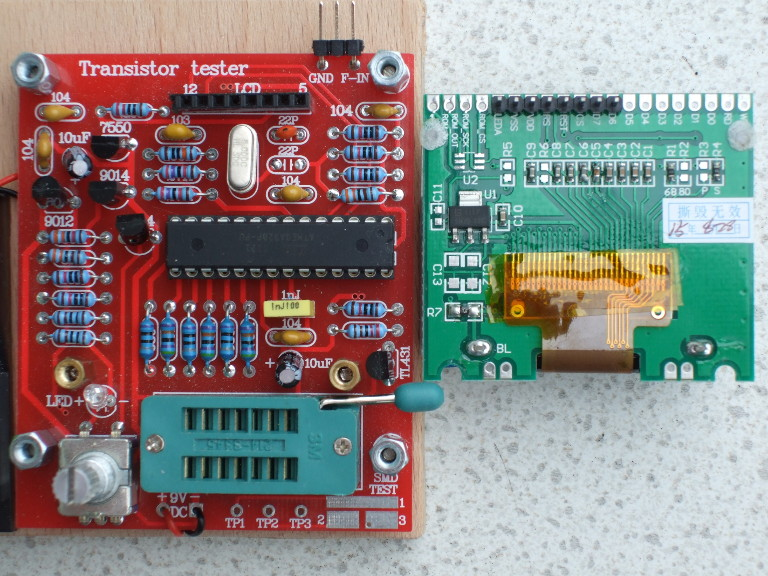
\includegraphics[width=9cm]{../PNG/Kit_ST7565b.jpg}
    \caption{with dismounted display}
  \end{subfigure}
  \caption{Assembled kit with 128x64 pixel display}
  \label{fig:Kit_mono}
\end{figure}

The later released kit use a color display with a ST7735 controller (160x128 pixel)
and is additionally equipped with a input for voltage measurement and a terminal for frequency output.
But the frequency output terminal is not buffered, it is simply connected parallel to the TP2 terminal.
The voltage measurement can handle positiv DC voltages up to 50V. A additional DC-DC converter
for the measurement of Zener diodes is not provided. 
The pictures~\ref{fig:Kit_color} shows this assembled kit.
Also in this version was one of the both \(22 pF\) capacitors replaced
by a trimmer (green color).

\begin{figure}[H]
  \begin{subfigure}[b]{9cm}
    \centering
    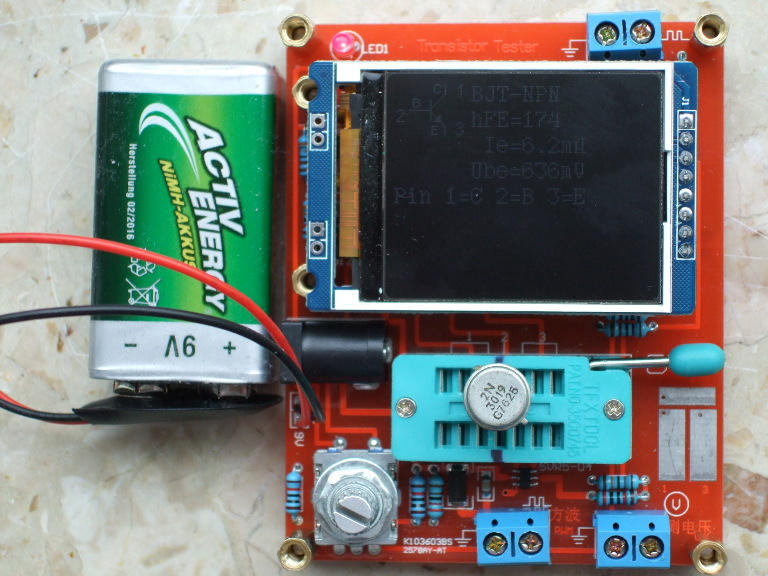
\includegraphics[width=9cm]{../PNG/Kit_Color_a.jpg}
    \caption{build together}
  \end{subfigure}
  ~
  \begin{subfigure}[b]{9cm}
    \centering
    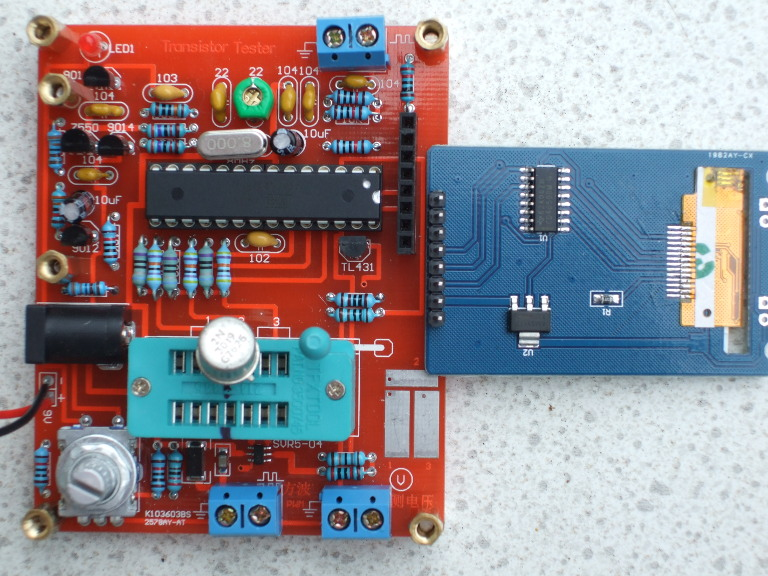
\includegraphics[width=9cm]{../PNG/Kit_Color_b.jpg}
    \caption{with dismounted display}
  \end{subfigure}
  \caption{Assembled kit with 160x128 pixel color display}
  \label{fig:Kit_color}
\end{figure}

Both kids use a DIP version of the ATmega328P mounted at a sockets and are
not equipped with a ISP connector for updating the ATmega with newer software versions.
The first version use
only leaded parts for the main circuit board. 
I have received measurement resistors \(680\Omega\) and \(470k\Omega\) with 0.1\% tolerance
with the Chinese kit. Also a \(220 nF\) capacitor for calibration was added
to the kit.
The kit with the color display was equipped with a connector for a DC power supply additionally
to the pads for the 9V battery.
Some few SMD parts was allready assembled at the main board, so that also only simple soldering
tasks are to do for this kit. 
A little disadvantage of the version with the color display is the speed of display output.
Especially for the menu handling the slower output speed will be noticed.
Otherwise the color display has a significant higher count of pixels, so more text can be shown at once.
Both kits use a 3.3V voltage regulator for the power of the display controller at the
full assembled display circuit boards.
Only the pin header must be soldered at the display circuit board.
The color version use a CD4050 buffer to adapt the different signal voltage levels.
I did not found any adaption of signal voltage levels at the board for the ST7565 version.
Probably the selected controller version tolerates the 5V signal levels of the ATmega328.
I could not find protection diodes at the input signals to the 3.3V supply side for this controller type.


\section{Extented circuit with ATmega644 or ATmega1284}

A extended circuit for ATmega644/1284 processors was developed with Nick L. from the Ukraine.
The circuit \ref{fig:t644tester} enables a additional test of crystals and a extended range
for the frequency measurement.
Although the basic circuit is very simular to the circuit \ref{fig:ttester}, the
port assignment is different.
A rotary pulse encoder with circuit \ref{fig:RotExt} can be connected here at the pins PB5 and PB7 (instead of PD1 and PD3).
Both signals and also the power signals VCC and GND are available at the ISP connector,
so that the extension can also be connected here.\\

The 16:1 frequency divider of the 74HC4060 is allways used for frequencies above \(2MHz\).
The frequency divider can also be used for frequencies between \(25kHz\) and \(400kHz\) to
upgrade the frequency resolution by using the period measurement.
For switching between the operational states (frequency divider and crystal oszillator)
the analog switches 74HC4052 are used.
The table \ref{tab:mega644-display} shows the pin assignments for the ATmega324/644/1284
microcontrollers for different display connections.
The using of the I\textsuperscript{2}C interface is only possible with the SSD1306 controller.
The signals of the I\textsuperscript{2}C interface require a pull-up resistor of \(4.7k\Omega\) to \(3.3V\).
The outputs of the ATmega is only switched to \(0V\) for the I\textsuperscript{2}C signals.


\begin{table}[H]
  \begin{center}
    \begin{tabular}{| c || c | c | c | c |}
    \hline
      Port & Character LCD &  Graphic LCD  & Graphic LCD  & additional function\\
           &               &  SPI 4-wire   &   I\textsuperscript{2}C        &            \\
    \hline
    \hline
    PB2    &  LCD-RS         &            &             &       \\
    \hline
    PB3    &  LCD-E          &  (LCD-CE)  &  LCD-SCL    &       \\
    \hline
    PB4    &  LCD-D4         &  LCD-REST  &  LCD-SDA    &       \\
    \hline
    PB5    &  LCD-D5         &  LCD-RS    &             & ISP-MOSI \\
           &                 &            &             & Rotary encoder 2 \\
    \hline
    PB6    &  LCD-D6         &  LCD-SCLK  &             & ISP-MISO \\
    \hline
    PB7    &  LCD-D7         &  LCD-SI    &             & ISP-SCK  \\
           &                 &            &             & Rotary encoder 1 \\
    \hline
    \end{tabular}
  \end{center}
  \caption{Different variations of the display port assignments}
  \label{tab:mega644-display}
\end{table}

You can also connect a display with the ST7108 controller ito the ATmega644 of ATmega1284 by using
a little circuit as shown in figure~\ref{fig:ST7108lcd_644}.
You should also respect the different pin assignments of display modules with ST7108 controllers as 
shown in table~\ref{tab:ST7108types} at page~\pageref{tab:ST7108types}.

\begin{figure}[H]
  \begin{subfigure}[b]{9cm}
    \centering
    
\includegraphics[width=8cm]{../FIG/ST7108serial164_644.eps}
    \caption{with 74HCT164}
  \end{subfigure}
  ~
  \begin{subfigure}[b]{9cm}
    \centering
    
\includegraphics[width=8cm]{../FIG/ST7108serial595_644.eps}
    \caption{with 74HCT595}
  \end{subfigure}
  \caption{Connection of a ST7108 Controller to a ATmega644/1284}
  \label{fig:ST7108lcd_644}
\end{figure}


\begin{figure}[H]
\centering

\includegraphics[width=18cm]{../FIG/t644tester.eps}
\caption{Extended Transistor Tester circuit with ATmega644}
\label{fig:t644tester}
\end{figure}


\section{Buildup of a tester with ATmega1280 or Arduino Mega}
The basic circuit of the tester can also be also build with a Arduino Mega with a ATmega1280
or ATmega2560 microcontroller with a shield.
The required connections are shown in figure~\ref{fig:t1280tester}.
The names for the connections of the display signals of the Arduino are shown with green color.
Components with red color identification are not required for operating.
The ATmega2560 controller has many connectors, but only one connector has the required
functions for both techniques of the frequency measurement.
The connector must be used as clock input for a build in counter and must also be 
used as interrupt source for change of signal level.
This feature is only available for the pin PE6 (T3/INT6).
The other clock inputs of counters PD7 (T0), PD6 (T1), PH7 (T4) and PL2 (T5) can not be 
used as interrupt source for status change.
Unfortunately the PE6 pin is not connected to a pin of the Arduino female connector strip.
The PE5 pin (7) is connected to the connector 3 of the PWM socket strip and
can be jumpered with the PE6 pin (8) of the ATmega2560.
The output signal of the frequency generation is available at the PB6 (OC1B) pin.
This pin is connected to the connector 12 of the PWM socket strip.
The ISP-connector is not required, because the program can be loaded with the bootloader
and the USB interface to the ATmega. With the bootloader there is always a
little delay for the power up start of the program.

\begin{figure}[H]
\centering

\includegraphics[width=18cm]{../FIG/t1280tester.eps}
\caption{TransistorTester circuit with ATmega1280, ATmega2560 or Arduino Mega}
\label{fig:t1280tester}
\end{figure}

Of course you can connect all supported displays also to the ATmega1280 or ATmega2560
as shown in table~\ref{tab:display-1280} .

\begin{table}[H]
  \begin{center}
    \begin{tabular}{| c || c | c | c | c | c | c |}
    \hline
           & Character     &  ST7565     & ST7920       & ST7108       & SSD1306     & additional function \\
      Port & LCD           &    SPI      & seriell      & seriell      &    I\textsuperscript{2}C      & \\
    \hline
    \hline
    PA0    &  LCD-D4       &   LCD-REST  &  LCD-RESET   & HC595-RCK      &             & \\
    \hline
    PA1    &  LCD-D5       &   LCD-RS    &              & LCD-CS2        &             & rotary encoder 2 \\
    \hline
    PA2    &  LCD-D6       &   LCD-SCLK  &              & HC164-CLK      &             & \\
    \hline
    PA3    &  LCD-D7       &   LCD-SI    &              & LCD-CS1        &             & rotary encoder 1 \\
    \hline
    PA4    &  LCD-RS       &             &   LCD-B0     & LCD-RS         &   LCD-SDA   & \\
           &               &             &              & HC164-SER      &             & \\
    \hline
    PA5    &  LCD-E        &   (LCD-CE)  &   LCD-EN     & LCD-EN         &   LCD--SCL  & \\
    \hline
    PA7    &  key signal   &             &              &                &             & \\
    \hline
    \end{tabular}
  \end{center}
  \caption{Connections for different display to the ATmega1280/2560 processors}
  \label{tab:display-1280}
\end{table}


\section{Programming of the microcontroller}
I release the software for the microcontroller with source code.
The developement is done with Linux operationg system (Ubuntu) and
is controlled with a Makefile. The Makefile makes sure, that your
software will be compiled with the prior selected Makefile options. Some constellations
are precompiled with the source. Please take a look to the ReadMe.txt file
in the directory Software/default and to the chapter~\ref{sec:config} at page~\pageref{sec:config}.
The result of compilation have the extensions .hex and .eep .
Usually the names will be TransistorTester.hex and TransistorTester.eep .
The .hex file contains the data for the program memory (flash) of the ATmega processor.
The .eep file contains the data for the EEprom memory of the ATmega. Both data files
must be loaded to the correct memory.

Additionally the operating state of the
ATmega processor must be programmed with the ``fuses''.
If you can use my Makefile and additionally the program avrdude \cite{avrdude}, you need no exact
knowledge of the details about the fuses. You have only to type ``make fuses'' if you
have no crystal or ``make fuses-crystal'' if you have installed the \(8MHz\) crystal to your printed board.
With the ATmega168 series of the microcontroller you can also use ``make fuses-crystal-lp'' to use
a crytal with the low power mode.
Never choose the crystal mode of clock generation, if you don't have installed
the \(8MHz\) crystal. If you are not sure with the fuses, leave them as default
set by manufactor and first bring the the tester to operation in this mode.
Maybe your program runs too slow, if you use program data compiled for
\(8MHz\) operation, but you can correct this later! But a wrong set of fuses may inhibit
later ISP-programming.

\subsection{Using the Makefile with Linux}
You can install packages with Debian based Linux versions by using a package manager as synaptic or dpkg.
The package ``subversion'' must be installed for downloading the sources or the documentation from the SVN archive.
With the command \\
``svn checkout svn://www.mikrocontroller.net/transistortester'' \\
you can download the complete archive.
Of course you can also download only subdirectories of the archive.
For using the Makefile in one of the subdirectories you must install the packages
make, binutils-avr, avrdude, avr-libc and gcc-avr.
Once you must prepare the access to the interfaces for the user.
If you open a consol window and you have also connected a ISP programmer with USB interface,
you can see the recognized USB devices with the command ''lsusb''.
A sample of the result of lsusb you can see here:
\begin{verbatim}
Bus 001 Device 001: ID 1d6b:0002 Linux Foundation 2.0 root hub
Bus 002 Device 003: ID 046d:c050 Logitech, Inc. RX 250 Optical Mouse
Bus 002 Device 058: ID 03eb:2104 Atmel Corp. AVR ISP mkII
Bus 002 Device 059: ID 2341:0042 Arduino SA Mega 2560 R3 (CDC ACM)
Bus 002 Device 001: ID 1d6b:0001 Linux Foundation 1.1 root hub
\end{verbatim}
A Device 58 is detected here a a AVR ISP mkII type (DIAMEX ALL-AVR).
The ID 03eb is a vendor ID and the ID 2104 is a product ID.
Both ID's are required for a entry in the file /etc/udev/rules.d/90-atmel.rules .
In this example the file 90-atmel.rules has one line:
\begin{verbatim}
SUBSYSTEM=="usb", ATTRS{idVendor}=="03eb", ATTRS{idProduct}=="2104", MODE="0660",
GROUP="plugdev"
\end{verbatim}
This entry allow the access to the USB device 58 for members of the group ''plugdev''.
The also detected USB device 59 allows a access to the serial device ''/dev/ttyACM0'' for
members of the group ''dialout''.

Therefore your user identification should be a member of the group plugdev and also
a member of the group dialout.
With the command ''usermod -a -G dialout,plugdev \$USER'' the membership of both groups should be established.
Now the program avrdude should have permission to access both devices.
In a console window you must first change the directory with the command ``cd'' to a proper
subdirectory of the directory trunk.
Now you can change options of the Makefile with any text editor.
For compiling the source you must only type the simple command ``make''.
If the ISP programmer is configured proper in the Makefile, a command ``make upload''
should result to load the program with the ISP interface to the ATmega.
The ``fuses'' of the ATmega must also be set correctly once.
You can achieve this with the command ``make fuses'' or ``make fuses-crystal''.
The program avrdude probably reports a error for setting the extended fuse efuse.
The reading of unused fuse bits is specified as ''1'' for the ATmega, but the
avrdude program mask the unused bits, so that it expect a ''0'' for all unused bits.
Normally the efuse should be set to 0xfc, but avrdude read back 0x04 with the mask.
You can change the file avrdude.conf to change the behaviour of avrdude or
you can set the efuse to 0x04. 
The value for all efuses can be set with the identifier EFUSE\_VAL at the begin of file setup.mk
in the trunk directory.
Probably the fuses are also set correctly with the error message.

\subsection{Using the WinAVR package with Windows}
If you use the Windows operating system, the easiest way to get a correct programmed
ATmega is to use the WinAVR package \cite{winavr1},\cite{winavr2}.
With my patch \cite{winavr3} you can also set the fuses by using the Makefile.
Of course the avrdude program must support your programmer and the configuration
in the Makefile must match to your environment.

The figures \ref{fig:WinAVR1} show the File menu of the graphical user interface of WinAVR for
open the file Makefile and for saving the changed Makefile (Save).

\begin{figure}[H]
  \begin{subfigure}[b]{9cm}
    \centering
    \includegraphics[width=9cm]{../PNG/Notepad_open.png}
    \caption{open Makefile}
  \end{subfigure}
  ~
  \begin{subfigure}[b]{9cm}
    \centering
    \includegraphics[width=9cm]{../PNG/Notepad_save.png}
    \caption{save Makefile}
  \end{subfigure}
  \caption{Using of the WinAVR user interface Programmer's Notepad}
  \label{fig:WinAVR1}
\end{figure}

The next figures \ref{fig:WinAVR2} show the Tools menu of the Programmer's Notepad
for compiling the program (Make All) and for programming the ATmega (Program) with avrdude.

\begin{figure}[H]
  \begin{subfigure}[b]{9cm}
    \centering
    \includegraphics[width=9cm]{../PNG/Notepad_make.png}
    \caption{Build programming data (.hex/.eep)}
  \end{subfigure}
  ~
  \begin{subfigure}[b]{9cm}
    \centering
    \includegraphics[width=9cm]{../PNG/Notepad_program.png}
    \caption{Programming the ATmega}
  \end{subfigure}
  \caption{Using of the WinAVR user interface Programmer's Notepad}
  \label{fig:WinAVR2}
\end{figure}



\section{Troubleshooting}
In most cases of problems you will miss the text output to the LCD-display.
At first you should check, if the LED was illuminated weak, if you release
the Test button. 
\begin{description}

\item[Power does not switch on.]
If the LED is without light and the VCC power has correct
\(5V\) voltage during holding the Test button, the microcontroller does not switch the power
correctly. The microcontroller should hold the power by switching the
PD6 output to \(5V\), which is usually done as one of the first actions.
If you hold the Test key pressed, the power is switched on anyway.
So you can check the value of VCC power and additionally the voltage value
of the PD6 output, if you hold the key pressed.
If VCC voltage has correct value (\(5V\)), but PD6 voltage is
below \(4V\), your microcontroller does not start the program. In this case
you should check if the microcontroller flash has been loaded with proper data for your
installed type and if ATmega is correctly configured with the fuses.
If your ATmega put the PD6 output to \(5V\) and the power does not stay if you
release the Test key, it is more difficult to find the reason.
First you can shorten the LED and try again. If your Tester now starts,
your LED may be faulty or mounted with wrong polarity. If this is not
the reason, the current amplification factor of your T3 transistor (BC557C)
is insufficient. The current to the base of T3 is lower in the microcontroller
state as in the ``key pressed'' state.

\item[Nothing is readable on the LCD display]
Check the voltage at the contrast pin at the LCD display (pin 3). Adjust to
correct value specified in the data sheet of your display and optimize by viewing.
If you have a high temperature display type, you must provide a negative contrast voltage
for operation. In this case you can use the ICL~7660 device for generating
a negative voltage from positive \(5V\).

The tester software can be configured for many different controller with different connection
types. You should check, if your software matches to your mounted display type.
If there is no output readable on the LCD and the background light is on,
you should disconnect the power and check all four data plus the two control signal connections.
If all connection are well, the only reason I see is a uncorrect timing of
control signals. This can be caused by a slower LCD controller than expected by
the software or the ATmega software runs at wrong clock speed. Please check for which
clock speed your programming data was compiled  and if the fuses of the
ATmega are correct set to that speed. You find the clock parameter in the corresponding
Makefile.
If the tester is build without the switch off electronic, you can test with
a LED connected to the test pins, if the program operates normally.
If the LED flickers, the program operates well. The missing text on the
LCD must be caused by wrong connection or timing.
For some graphical displays the contrast is changeable with a menu function.
If you have changed the contrast value, that nothing is readable at the screen,
you cannot handle the menu function any more. You can try to read the display
from a slanting look to the display, not from the front side.
In this case you can try to handle the menu function with this view.
Otherwise you can write the EEprom data new with a ISP programmer to reset the contrast value.


\item[Something but not all is readable on the LCD display]
Check if the .eep data are loaded to the EEprom memory of ATmega.
If all data are loaded correctly, you should check the clock speed of your
programming data (Makefile) and ATmega processor settings (fuses).

\item[Measurement is slow and Capacitors are measured about 8 times too small]
You run software compiled for \(8MHz\) clock at real clock speed of \(1MHz\).
Please set the fuses of the ATmega correctly.

\item[Measurement has strangely values]
Check if your programmer is still connected to the ISP-plug.
The ISP interface should be disconnected for measuring.
Very often the reason of wrong measurements is the use of software compiled with
the AUTOSCALE\_ADC option and with the option NO\_REF\_CAP, but the capacitor
at the AREF pin has still a value of \(100nF\).
Wrong assembly of components or remaining soft solder flux can disturb the 
measurements too. Please check with the selftest function of your TransistorTester software
if possible. For the details see Chapter \ref{sec:selftest}.

Otherwise inspect your board visually and check the resistor values
with a ohmmeter. You can use the pins of the ATmega for this check, for example
to check the R1 you can measure between pin 23 and pin 14. Take a look at the
circuit diagram \ref{fig:ttester} for details. There is no need to
remove the microcontroller, only battery or power supply should be removed before.

\item[The Tester switch off the power after 2 seconds display time] 
This condition exists, if the external Pull-Up resistor at the PD7 input
is missing or the key button is keep pressed.
The software switch off the internal Pull-Up resistors to prevent a influence
to the measurement results. Therefore a external Pull-Up resistor (27k) is required.

\item[Der Tester shows only Vext=xx.xV in row 2]
This problem exists, if the Pull-Up resistor at the PD7 input
is missing or the key button is keep pressed.
Additionally the software is configured without the serial output (without option WITH\_UART) and
without the internal Pull-Up resistors (with option PULLUP\_DISABLE).
You should install the Pull-Up resistor at pin PD7.


\end{description}


\chapter{Bedienungshinweise}
\label{sec:manual}
\section{Der Messbetrieb}
Die Bedienung des Transistortesters ist einfach.
Trotzdem sind einige Hinweise erforderlich.
Meistens sind an die drei Testports über Stecker-Leitungen mit Krokodilklemmen oder anderen Klemmen angeschlossen.
Es können auch Fassungen für Transistoren angeschlossen sein.
In jedem Fall können Sie Bauteile mit drei Anschlüssen mit den drei Testports in beliebiger Reihenfolge verbinden.
Bei zweipoligen Bauteilen können Sie die beiden Anschlüsse mit beliebigen Testports verbinden.
Normalerweise spielt die Polarität keine Rolle, auch Elektrolytkondensatoren können beliebig angeschlossen werden.
Die Messung der Kapazität wird aber so durchgeführt, dass der Minuspol am Testport mit der kleineren Nummer liegt.
Da die Messspannung aber zwischen \(0,3V\) und maximal \(1,3V\) liegt, spielt auch hier die Polarität keine wichtige Rolle.
Wenn das Bauteil angeschlossen ist, sollte es während der Messung nicht berührt werden. Legen Sie es auf einen
isolierenden Untergrund ab, wenn es nicht in einem Sockel steckt. Berühren Sie auch nicht die Isolation der Messkabel,
das Messergebnis kann beeinflusst werden.
Dann sollte der Starttaster gedrückt werden.
Nach einer Startmeldung erscheint nach circa zwei Sekunden das Messergebnis. Bei einer Kondensatormessung kann es
abhängig von der Kapazität auch deutlich länger dauern.

Was dann weiter geschieht, hängt von der Softwarekonfiguration des Testers ab.
\begin{description}
  \item[Einzelmessung] Wenn der Tester für Einzelmessung konfiguriert ist (POWER\_OFF-Option),
 schaltet der Tester nach einer Anzeigezeit
von 28 Sekunden (konfigurierbar) wieder automatisch aus, um die Batterie zu schonen.
Während der Anzeigezeit kann aber auch vorzeitig eine neue Messung gestartet werden.
Nach der Abschaltung kann natürlich auch wieder eine
neue Messung gestartet werden, entweder mit dem gleichen Bauteil oder mit einem anderen Bauteil.
Wenn die Elektronik zum Abschalten fehlt, wird das letzte Messergebnis weiter angezeigt.

  \item[Dauermessung] Einen Sonderfall stellt die Konfiguration ohne die automatische Abschaltfunktion dar.
Hierfür wird die POWER\_OFF-Option in der Makefile nicht gesetzt.
Diese Konfiguration wird normalerweise nur ohne die Transistoren für die Abschaltung benutzt.
Es wird stattdessen ein externer Ein-/Aus-Schalter benötigt. Hierbei wiederholt der Tester die
Messungen solange, bis ausgeschaltet wird.

  \item[Serienmessung] In diesem Konfigurationsfall wird der Tester nicht nach einer Messung sondern erst nach einer konfigurierbaren
Zahl von Messungen abgeschaltet. Hierfür wird der POWER\_OFF-Option in der Makefile eine Wiederholzahl (z.B. 5) zugewiesen.
Im Standardfall wird der Tester nach fünf Messungen ohne erkanntes Bauteil abgeschaltet.
Wird ein angeschlossenes Bauteil erkannt, wird erst bei der doppelten Anzahl, also zehn Messungen abgeschaltet.
Eine einzige Messung mit nicht erkanntem Bauteil setzt die Zählung für erkannte Bauteile auf Null zurück.
Ebenso setzt eine einzige Messung mit erkannten Bauteil die Zählung für die nicht erkannten Bauteile auf Null zurück.
Dies hat zur Folge, dass auch ohne Betätigung des Starttasters immer weiter gemessen werden kann,
 wenn Bauteile regelmässig gewechselt werden.
Ein Bauteilwechsel führt in der Regel durch die zwischenzeitlich leeren Klemmen zu einer Messung ohne erkanntes Bauteil.

Eine Besonderheit gibt es in diesem Betriebsmodus für die Anzeigezeit. Wenn beim Einschalten der Starttaster nur kurz
gedrückt wurde, beträgt die Anzeigezeit der Messergebnisse nur 5 Sekunden. Wenn der Starttaster bis zum Erscheinen der
ersten Meldung festgehalten wurde, beträgt die Anzeigezeit wie bei der Einzelmessung 28 Sekunden.
Ein vorzeitiger neuer Messbeginn ist aber während der Anzeigezeit durch erneutes Drücken des Starttasters möglich.

\end{description}

\section{Optionale Menüfunktionen für den ATmega328}
Wenn die Menüfunktion eingeschaltet ist, startet der Tester nach einem längeren Tastendruck (\textgreater~\(0.5s\)) ein Auswahlmenü
für zusätzliche Funktionen.
Diese Funktion ist auch für andere Prozessoren mit mindestens 32K Flash Speicher verfügbar.
Die wählbaren Funktionen erscheinen in Zeile~2 eines zweizeiligen Displays oder werden als gekennzeichnete
Funktion in Zeile 3 eines vierzeiligen Displays gezeigt. Dabei wird die vorige und nächste Funktion in Zeile 2 und 4 angezeigt.
Nach einer längeren Wartezeit ohne jegliche Bedienung kehrt das Programm zu der normalen Transistortester-Funktion zurück.
Durch kurzen Tastendruck kann zur nächsten Auswahl gewechselt werden.
Mit einem längeren Tastendruck startet die angezeigte Zusatzfunktion.
Nach Anzeige der letzten Funktion ,,Schalte aus'' wird wieder die erste Funktion angezeigt.\\

Wenn der Tester mit einem Drehimpulsgeber ausgerüstet ist, kann die Menü-Auswahl auch mit einem schnellen
Drehen des Encoders während der Anzeige einer vorausgegangenen Messung aufgerufen werden.
Die Menüfunktionen können mit einem langsamen Drehen des Encoders in beliebiger Richtung ausgewählt werden.
Die ausgewählte Menüfunktion kann aber nur mit einem längeren Tastendruck gestartet werden.
Innerhalb einer Menüfunktion können Parameter durch eine langsame Drehung des Encoders ausgewählt werden.
Eine schnelle Drehung des Encoders kehrt zur Menü-Auswahl zurück.

\begin{description}
 \item[Frequenz]
Die Zusatzfunktion ,,Frequenz'' (Frequenzmessung) benutzt als Eingang den PD4-Pin des ATmega, der auch an das LCD angeschlossen ist.
Es wird immer zunächst die Frequenz gemessen, bei Frequenzen unter \(25kHz\) wird auch die mittlere Periode des Eingangssignals
bestimmt und daraus die Frequenz mit einer Auflösung von bis zu \(0,001Hz\) berechnet.
Bei gesetzter POWER\_OFF-Option in der Makefile wird die Dauer der Frequenzmessung auf 8~Minuten beschränkt.
Die Frequenzmessung wird durch Tastendruck beendet und in das Auswahlmenü zurückgekehrt.\\

 \item[f-Generator]
Bei der Zusatzfunktion ,,f-Generator'' (Frequenz-Generator) können die Frequenzen zwischen 1Hz und 2MHz gewählt werden.
Die Einstellung der Frequenz kann jeweils nur für die höchste dargestellte Stelle (Ziffernposition) verändert werden.
Für die Stellen 1Hz bis 10kHz sind jeweils die Ziffern 0-9 wählbar. Bei der 100kHz Stelle ist 0-20 wählbar.
In Spalte 1 der Frequenzzeile wird durch ein \textgreater~oder \textless~Symbol angezeigt, ob durch einen längeren
Tastendruck (\textgreater~0.8s) zur höheren oder niedrigen Stelle geschaltet wird.
Zur niedrigeren Stelle (\textless) kann nur geschaltet werden, wenn die augenblickliche Stellee auf 0 gestellt wurde
und wenn nicht die Stelle mit 1Hz Schritten gewählt wurde.
Bei der gewählten 100kHz Stelle ist das \textgreater~Symbol durch ein R Zeichen ersetzt. Der längere Tastendruck bewirkt dann eine
Rücksetzung der Frequenz auf den Startwert 1Hz.
Bei gesetzter POWER\_OFF-Option in der Makefile muss für den Frequenzwechsel die Taste länger gedrückt werden, da
durch einen kurzen Tastendruck (\textless~0,2s) nur die Zeitüberwachung von 4~Minuten zurückgesetzt wird.
Die abgelaufene Zeit wird in Zeile 1 durch einen Punkt für jede abgelaufene 30 Sekunden angezeigt.
Durch einen regelmäßigen kurzen Tastendruck kann die vorzeitige Abschaltung der Frequenzerzeugung verhindert werden.
Ein längerer Tastendruck (\textgreater~1,4s) kehrt wieder zur Auswahl der Funktionen zurück.\\

 \item[10-bit PWM]
Bei der Zusatzfunktion ,,10-bit PWM'' (Pulsweitenmodulation) wird eine feste Frequenz mit einstellbarer Pulsweite an Pin TP2 erzeugt.
Mit einem kurzen Tastendruck (\textless~0,5s) wird die Pulsweite um \(1\%\) erhöht, mit einem längeren Tastendruck um \(10\%\).
Bei Überschreiten von \(99\%\) werden \(100\%\) vom erhöhten Wert abgezogen.
Bei gesetzter POWER\_OFF-Option in der Makefile wird die Frequenzerzeugung nach 8 Minuten ohne Bedienung beendet.
Durch sehr langen Tastendruck (\textgreater~1,3s) kann die Frequenzerzeugung auch beendet werden.\\

 \item[C+ESR@TP1:3]
Bei der Zusatzfunktion ,,C+ESR@TP1:3'' wird eine separate Kondensatormessung mit ESR-Messung an TP1 und TP3 gestartet.
Messbar sind Kondensatoren mit mehr als \(2\mu F\) bis zu \(50mF\). Wegen der geringen Messspannung von etwa 300mV sollte
in vielen Fällen die Messung in der Schaltung ohne vorherigen Ausbau möglich sein.
Bei gesetzter POWER\_OFF-Option in der Makefile ist die Anzahl der Messungen auf 250 beschränkt,
kann aber sofort wieder gestartet werden.
Die Mess-Serie kann durch einen längeren Tastendruck beendet werden.\\

 \item[Widerstandsmeßgerät]
Mit dem \mbox{1 \electricR 3} Symbol wird der Tester in ein Ohmmeter an TP1 und TP3 verwandelt. Diese Betriebsart wird durch
ein {\bf[R]} in der rechten Ecke der ersten Displayzeile angezeigt. Weil bei dieser Betriebsart die
ESR-Meßfunktion nicht benutzt wird, beträgt auch für Widerstände unter \(10\Omega\) die Auflösung
nur \(0.1\Omega\). Wenn die Ohmmeter Funktion mit der Induktitivitätsmessung konfiguriert wurde,
erscheint hier ein \mbox{1 \electricR \electricL 3} Symbol.
Dann beinhaltet die Ohmmeter Funktion die Messung von Induktivitäten für Widerstände unter \(2100\Omega\). 
In der rechten Ecke der ersten Zeile des Displays wird dann ein {\bf[RL]} angezeigt.
Für Widerstände unter \(10\Omega\) wird dann auch die ESR-Meßmethode benutzt,
wenn keine Induktivität festgestellt wurde. Damit erhöht sich die Auflösung für Widerstände
unter \(10\Omega\) auf \(0.01\Omega\).
In dieser Betriebsart werden die Meßwerte fortlaufend ermittelt.
Mit einem Tastendruck beendet der Tester diese Betriebsart und kehrt wieder zum Menü zurück.
Die gleiche Betriebsart wird auch automatisch gestartet, wenn zwischen TP1 und TP3 ein einzelner Widerstand
angeschlossen wurde und der Start-Taster gedrückt wurde. In diesen Fall kehrt der Tester mit einem Tastendruck 
wieder zu der normalen Teseterfunktion zurück.

 \item[Kondensatormeßgerät]
Mit dem \mbox{1 \electricC 3} Symbol wird der Tester
in ein reines Kondensator-Meßgerät an TP1 und TP3 verwandelt.
Die Betriebsart wird durch ein {\bf[C]} in der rechten Ecke der ersten Zeile des Displays angezeigt.
Bei dieser Betriebsart können Kondensatoren ab \(1pF\) bis zu \(100mF\) gemessen werden.
In dieser Betriebsart werden die Meßwerte fortlaufend ermittelt.
Mit einem Tastendruck wird dieser Sonderbetrieb beendet und der Tester kehrt wieder zum Menü zurück.
Auch hier wird wie bei der Widerstands-Meßfunktion in den  Betriebs-Modus automatisch gewechselt,
 wenn zwischen TP1 und TP3 ein Kondensator mit der normalen Testerfunktion gemessen wurde.
Der Tester kehrt nach dem automatischen Start wieder zu der normalen Testerfunktion zurück, wenn der Taster gedrückt wird.

 \item[Impulsdrehgeber]
Mit der Zusatzfunktion ,,Impulsdrehgeber'' kann ein Drehgeber untersucht werden.
Die drei Kontakte des Impulsdrehgebers müssen vor dem Start der Zusatzfunktion beliebig an die drei Testpins
 des Transistortesters angeschlossen werden.
Nach dem Start der Funktion muss der Drehknopf nicht zu schnell gedreht werden.
Wenn der Test erfolgreich abgeschlossen ist, wird die Pinbelegung der Kontakte symbolisch in Zeile 2 dargestellt.
Dabei wird der gemeinsame Anschluss herausgefunden und für etwa zwei Sekunden angezeigt,
ob an den Raststellung beide Kontake offen ('o') oder beide Kontakte geschlossen ('C') sind.
Ein Impulsdrehgeber mit offenen Kontakten an den Raststellungen wird so mit der Zeile 2 ,,1-/-2-/-3~o'' zwei Sekunden lang angezeigt.
Natürlich wird die richtige Pinnummer des gemeinsamen Kontaktes in der Mitte anstelle der '2' angezeigt.
Wenn auch die geschlossene Schalterstellung an den Raststellungen vorkommt,
wird außerdem in Zeile 2 ,,1---2---3~C'' zwei Sekunden lang angezeigt.
Mir ist kein Impulsdrehgeber bekannt, der immer nur geschlossene Kontakte an jeder Raststellung hat.
Die Stellungen der Kontakte zwischen den Raststellungen werden nur kurz (\textless\(~0,5s\)) ohne die Kennbuchstaben 'o' oder 'C' 
in Zeile 2 angezeigt.
Wenn der Impulsdrehgeber für die Bedienung des Testers eingesetzt werden soll, muß die Makefile Option WITH\_ROTARY\_SWITCH=2
für Drehgeber mit nur den offenen Kontakten ('o') und die Option WITH\_ROTARY\_SWITCH=1 für Drehgeber mit
offenen ('o') und geschlossenen ('C') Kontakten an den Raststellungen.\\

\item[C(\(\mu F\))-Korrektur]
Mit dieser Menüfunktion kann ein Korrekturwert für die Messung grösserer Kapazitätswerte geändert werden.
Die Funktion ist die gleiche, die auch mit der Makefile Option C\_H\_KORR voreingestellt werden kann.
Werte über Null reduzieren den Ausgabewert der Kapazität um diesen Prozent Wert, Werte unter Null würden den Ausgabewert
anwachsen lassen. Ein kurzer Tastendruck verringert den Korrekturwert um 0.1\%, ein längerer Tastendruck vergrößert
den Korrekturwert um 0.1\%. Ein sehr langer Tastendruck speichert den Wert.  Es ist eine Eigenschaft des
Meßverfahrens, daß Kondensatoren mit geringer Güte wie Elektrolyt-Kondensatoren mit zu großer Kapazität gemessen werden.
Erkennbar ist die Güte über den Parameter Vloss. Gute Kondensatoren haben kein Vloss oder nur 0.1\%.
Zum Abgleich dieses Parameters sollten also nur Kondensatoren mit über \(50\mu F\) hoher Güte verwendet werden.
Übrigens halte ich die Bestimmung des exakten Kapazitätswertes von Elektrolyt-Kondensatoren für überflüssig,
da die Kapazität sowohl von der Temperatur als auch der DC-Spannung abhängt.

 \item[Selbsttest]
Mit der Zusatzfunktion ,,Selbsttest'' wird ein vollständiger Selbsttest mit Kalibration durchgeführt.
Dabei werden sowohl die Testfunktionen T1 bis T7 (wenn nicht verhindert mit der Option NO\_TEST\_T1\_T7) 
als auch die Kalibration mit dem externen Kondensator jedes Mal durchgeführt.\\

 \item[Spannung]
Die Zusatzfunktion ,,Spannung'' (Spannungsmessung) ist nur möglich, wenn die serielle Ausgabe deaktiviert wurde
oder der ATmega mindestens 32 Pinne hat (PLCC) und einer der zusätzlichen Pinne ADC6 oder ADC7 für die Messung benutzt wird.
Da am Port PC3 (oder ADC6/7) ein 10:1-Spannungsteiler vorgesehen ist, können Spannungen bis \(50V\) gemessen werden.
Ein installierter DC-DC-Wandler für die Zenerdioden-Messung wird durch Tastendruck eingeschaltet.
So können auch angeschlossene Zenerdioden gemessen werden.
Bei gesetzter POWER\_OFF-Option in der Makefile und ohne Bedienung wird die Messung nach 4~Minuten beendet.
Die Messung kann aber durch einen besonders langen Tastendruck (\textgreater~4~Sekunden) vorher beendet werden.\\

\item[Kontrast] 
Diese Funktion steht für Controller mit Kontrasteinstellung per Software zur Verfügung.
Der Einstellwert kann mit einem sehr kurzen Tastendruck oder einer Linksdrehung des Impulsdrehgebers verringert werden.
Ein längerer Tastendruck oder eine Rechtsdrehung des Impulsdrehgebers vergrößert den Einstellwert.
Die Funktion wird beendet und der eingestellte Wert wird permanent in den EEPROM geschrieben, 
wenn die Taste noch länger gedrückt wird.

\item[BackColor]
Für Farbdisplays kann dieser Menüpunkt mit der Makefile Option LCD\_CHANGE\_COLOR eingeschaltet werden,
um die Hintergrundfarbe einstellen zu können. Die Impulsdrehgeber-Erweiterung muß dafür installiert sein.
Sie können eine der drei Farben rot, grün und blau mit einem längeren Tastendruck wählen.
Die Intensität der gewählten Farbe, die mit einem > Zeichen in Spalte 1 gekennzeichnet wird,
kann durch Drehen des Impulsdrehgebers verändert werden.

\item[FrontColor]
Für Farbdisplays kann dieser Menüpunkt mit der Makefile Option LCD\_CHANGE\_COLOR eingeschaltet werden,
um die Vordergrundfarbe einstellen zu können. Die Impulsdrehgeber-Erweiterung muß dafür installiert sein.
Sie können eine der drei Farben rot, grün und blau mit einem längeren Tastendruck wählen.
Die Intensität der gewählten Farbe, die mit einem > Zeichen in Spalte 1 gekennzeichnet wird,
kann durch Drehen des Impulsdrehgebers verändert werden.

 \item[Zeige Daten]
Die Funktion ,,Zeige Daten'' zeigt neben der Software-Versionsnummer die Daten des Abgleichs an.
Dies sind die Nullwiderstände R0 von Pin 1:3, 2:3 und 1:2 .
Außerdem werden die Ausgangswiderstände der Ports zur \(5V\)-Seite (RiHi) und 
zur \(0V\) Seite (RiLo) angezeigt.
Die Nullkapazitätswerte (C0) werden ebenfalls in allen Pinkombinationen angezeigt (1:3, 2:3, 1:2 und 3:1, 3:2 2:1).
Danach werden auch die Spannungskorrekturen für die Komparatorspannung (REF\_C) und für die Referenzspannung (REF\_R) angezeigt.
Bei Graphikdisplays werden danach noch die verwendeten Symbole für die Bauteile und der Fontsatz angezeigt.
Jede Seite wird 15 Sekunden angezeigt.
Es kann aber auch durch Tastendruck oder einer Rechtsdrehung des Impulsdrehgebers
zur nächsten Seite geblättert werden.
Mit einer Linksdrehung des Impulsdrehgebers kann die Ausgabe wiederholt werden oder zur vorigen Seite zurückgeblättert werden.

 \item[Schalte aus]
Mit der Zusatzfunktion ,,Schalte aus'' kann der Transistortester abgeschaltet werden.\\

 \item[Transistor]
Natürlich kann mit der Funktion ,,Transistor'' (Transistortester) wieder zu der normalen Transistortester-Funktion
zurückgekehrt werden.

\end{description}

Bei gesetzter POWER\_OFF-Option in der Makefile sind alle Zusatzfunktionen zeitbeschränkt, damit die Batterie nicht verbraucht wird.

\section{Selbsttest und Kalibration}

Wenn die Software mit der Selbsttestfunktion konfiguriert ist, kann der Selbsttest durch einen Kurzschluss aller drei
Testports und Drücken der Starttaste eingeleitet werden.
Für den Start des Selbsttests muss die Starttaste innerhalb von 2 Sekunden noch einmal gedrückt werden,
sonst wird mit einer normalen Messung fortgefahren.
Beim Selbsttest werden die im Selbsttest-Kapitel \ref{sec:selftest} beschriebenen Tests ausgeführt.
Wenn der Tester mit einer Menüfunktion (Option WITH\_MENU) konfiguriert ist, 
wird der vollständige Selbsttest mit den Tests T1 bis T7 nur bei dem ,,Selbsttest'' ausgeführt, 
der als Menüfunktion ausgewählt werden kann.
Außerdem wird beim Aufruf über die Menüfunktion der Abgleich mit dem externen Kondensator jedesmal durchgeführt,
sonst nur für den ersten Aufruf.
Damit kann der durch die kurgeschlossenen Testports automatisch gestartete Abgleich schneller durchgeführt werden. 
Die viermalige Testwiederholung bei T1 bis T7 kann vermieden werden, wenn der Starttaster gedrückt gehalten wird.
So kann man uninteressante Tests schnell beenden und
sich durch Loslassen des Starttasters interessante Tests viermal wiederholen lassen.
Der Test 4 läuft nur automatisch weiter, wenn die Verbindung zwischen den Testports gelöst wird.

Wenn die Funktion AUTO\_CAL in der Makefile gewählt ist, wird beim Selbsttest
eine Kalibration der Nullwertes für die Kondensatormessung durchgeführt.
Für die Kalibration des Nullwertes für die Kondensatormessung ist wichtig, 
dass die Verbindung zwischen den Testpins (Kurzschluß) während des Tests 4 wieder gelöst wird!
Sie sollten während der Kalibration (nach dem Test 6) weder die Testports noch angeschlossene Kabel berühren.
Die Ausrüstung sollte aber die gleiche sein, die später zum Messen verwendet wird.
Anderenfalls wird der Nullwert der Kondensatormessung nicht richtig bestimmt.
Die Kalibration des Innenwiderstandes der Port-Ausgänge wird mit dieser Option vor jeder
Messung durchgeführt. \\

Bei der Kalibration werden zwei Sonderschritte gemacht, wenn die samplingADC Funktion in der Makefile gewählt wurde (WITH\_SamplingADC = 1).
Nach der normalen Bestimmung der Nullwerte der Kapazitätsmessung werden dann auch die Nullwerte mit
der Sampling Methode (C0samp) bestimmt. Als letzter Teil der Kalibration wird der Anschluß eines Testkondensators für die
Spulenmessung an Pin~1 und Pin~3 angefordert mit der Meldung \mbox{1 \electricC 3  10-30nF(L)}.
Der Kapazitätswert sollte hierbei zwischen \(10nF\) und \(30nF\) liegen,
um eine meßbare Resonanzfrequenz bei der späteren Parallelschaltung mit einer Spule (\textless~\(2mH\)) zu erreichen.
Für Spulen mit mehr als 2mH Induktivität sollte die normale Testfunktion ohne die Parallelschaltung eines
Kondensators ausreichen. Ein Parallelschalten des Kondensators sollte hier nicht mehr 
zu einer Verbesserung des Meßergebnisses führen.\\

Nach der Bestimmung der Nullkapazitäten ist der Anschluss eines Kondensators 
mit einer beliebiger Kapazität zwischen \(100nF\) und \(20\mu F\) an Pin~1 und Pin~3 erforderlich.
Dazu wird in Zeile 1 ein \mbox{1 \electricC 3\textgreater 100nF} angezeigt.
Sie sollten den Kondensator erst nach der Ausgabe der C0 Werte oder nach der Ausgabe dieser Aufforderung anschließen.
Mit diesem Kondensator wird die Offset-Spannung des analogen Komparators kompensiert,
um genauere Kapazitätswerte ermitteln zu können.
Die Verstärkung für ADC-Messungen mit der internen Referenz-Spannung wird ebenfalls mit diesem Kondensator abgeglichen, um
bessere Widerstands-Messergebnisse mit der AUTOSCALE\_ADC-Option zu erreichen.
Wenn die Menüfunktion beim Tester ausgewählt wurde (Option WITH\_MENU) und der Selbsttest
nicht als Menüfunktion gestarte wurde, wird der Abgleich mit dem externen Kondensator nur bei
der ersten Kalibration durchgeführt.
Die Kalibration mit dem externen Kondensator kann nur wiederholt werden, wenn der Selbsttest
als Menüfunktion ausgewählt wird.

Der Nullwert für die ESR-Messung wird als Option ESR\_ZERO in der Makefile vorbesetzt.
Mit jedem Selbsttest wird der ESR Nullwert für alle drei Pinkombinationen neu bestimmt.
Das Verfahren der ESR-Messung wird auch für Widerstände mit Werten unter \(10\Omega\) benutzt um
hier eine Auflösung von \(0,01\Omega\) zu erreichen.

\section{Besondere Benutzungshinweise}
Normalerweise wird beim Start des Testers die Batteriespannung angezeigt. Wenn die Spannung eine Grenze unterschreitet, 
wird eine Warnung hinter der Batteriespannung ausgegeben. Wenn Sie eine aufladbare \(9V\)-Batterie benutzen, sollten Sie
den Akku möglichst bald austauschen oder nachladen.
Wenn Sie eine Version mit eingebauter \(2,5V\)-Präzisionsreferenz besitzen, wird beim Start für eine Sekunde die
gemessene Betriebsspannung in der Zeile 2 mit ,,VCC=x.xxV'' angezeigt.

Es kann nicht oft genug erwähnt werden, dass Kondensatoren vor dem Messen entladen sein müssen.
Sonst kann der Tester schon defekt sein, bevor der Startknopf gedrückt ist.
Wenn man versucht, Bauelemente im eingebauten Zustand zu messen, sollte das Gerät immer von
der Stromquelle getrennt sein. Außerdem sollte man sicher sein, dass keine Restspannung mehr
im Gerät vorhanden ist. Alle Geräte haben Kondensatoren verbaut!

Beim Messen kleiner Widerstandswerte muss man besonders auf die Übergangswiderstände achten.
Es spielt die Qualität und der Zustand von Steckverbindern eine große Rolle, genau so wie die
Widerstandwerte von Messkabeln. Dasselbe gilt auch für die Messung des ESR-Wertes von Kondensatoren.
Bei schlechten Anschlusskabeln mit Krokodilklemmen wird so aus einem ESR von \(0,02\Omega\) leicht
ein Wert von \(0,61\Omega\).
Wenn möglich sollte man Kabel mit Testklemmen an die drei Testports parallel zu vorhandenen Sockeln fest anschließen (anlöten).
Dann braucht der Tester für kleine Kapazitäten nicht jedesmal neu kalibriert werden, wenn mit oder ohne eingesteckte
Testkabel gemessen wird. Für die Kalibration des Nullwiderstandes macht es aber im allgemeinen einen Unterschied, 
ob die Testpins direkt am Sockel oder am Ende der Kabel mit den den Testklemmen verbunden wird. Nur im letzteren
Fall ist der Widerstand von Kabel und Klemmen mit kalibriert. Im Zweifelsfall kann man die Kalibration mit dem
Kurzschluß am Testsockel durchführen und danach den Widerstand der kurzgeschlossenen Klemmen mit dem Tester messen.

An die Genauigkeit der Messwerte sollte man keine übertriebenen Erwartungen haben, dies gilt besonders
für die ESR Messung und die Induktivitätsmessung.
Die Ergebnisse meiner Messreihen kann man im Kapitel \ref{sec:measurement} ab Seite~\pageref{sec:measurement} finden.



\section{Problemfälle}
Bei den Messergebnissen sollten Sie immer im Gedächtnis behalten, dass die Schaltung des Transistortesters für
Kleinsignal-Bauelemente ausgelegt ist. Normalerweise beträgt der maximale Messstrom etwa \(6mA\).
Leistungshalbleiter machen oft wegen hoher Reststöme Probleme bei der Erkennung oder beim Messen der
Sperrschicht-Kapazität.
Bei Thyristoren und Triacs werden oft die Zündströme oder die Halteströme nicht erreicht. Deswegen kann es
vorkommen, dass ein Thyristor als NPN-Transistor oder Diode erkannt wird. Ebenso ist es möglich, dass ein 
Thyristor oder Triac gar nicht erkannt wird.

Probleme bei der Erkennung machen auch Halbleiter mit integrierten Widerständen.
So wird die Basis-Emitter-Diode eines BU508D-Transistors wegen eines parallel geschalteten internen
\(42 \Omega\) Widerstandes nicht erkannt.
Folglich kann auch die Transistorfunktion nicht geprüft werden.
Probleme bei der Erkennung machen oft auch Darlington-Transistoren höherer Leistung. Hier sind auch
oft Basis-Emitter-Widerstände verbaut, welche die Erkennung wegen der hier verwendeten kleinen Messströme erschweren.

\section{Messung von PNP- und NPN-Transistoren}
Normalerweise werden die drei Anschlüsse des Transistors in beliebiger Reihenfolge an die Messeingänge des
Transistortesters angeschlossen.
Nach dem Drücken des Starttasters meldet der Tester in der Zeile 1 den Typ (NPN oder PNP), 
eine eventuell vorhandene Schutzdiode der Kollektor-Emitter-Strecke und
die Anschlussbelegung. Das Diodensymbol wird  polungsrichtig angezeigt.
In der Zeile 2 wird der Stromverstärkungsfaktor \(B\) oder \(hFE\) angegeben und der Strom, bei der die Verstärkung
bestimmt wurde. Wenn die Emitterschaltung für die Bestimmung des Verstärkungsfaktors verwendet wurde,
wird der Kollektorstrom \(Ic\) genannt. Bei Bestimmung des Verstärkungsfaktors in Kollektorschaltung (Emitterfolger)
wird der Emitterstrom \(Ie\) angegeben. Weitere Parameter werden bei einem zweizeiligen Display
nacheinander in Zeile 2 angegeben. Bei Displays mit mehr Zeilen werden weitere Zeilen benutzt bis
die letzte Zeile schon benutzt war.
Erst bei der letzten Zeile erfolgen weitere Ausgaben nacheinander in der letzten Zeile.
Wenn weitere Parameter vorhanden sind, wird am Ende der letzten Zeile ein + Zeichen ausgegeben.
Der nächste Wert erscheint auf Knopfdruck oder nach einer Wartezeit auch automatisch.
Der nächste ausgegebene Parameter ist jedenfalls die Basis-Emitter-Schwellspannung \(Ube\),
bei der der Verstärkungsfaktor bestimmt wurde.
Falls meßbar, werden auch der Kollektor-Reststrom mit offener Basis \(I_{CE0}\) und mit kurzgeschlossener
Basis \(I_{CES}\) ausgegeben.
Falls eine Schutzdiode vorhanden ist, wird die Flußspannung \(Uf\) dieser Schutzdiode als letzter Parameter ausgegeben.


Bei der Emitterschaltung hat der Tester nur zwei Möglichkeiten, den Basisstrom einzustellen:
\begin{enumerate}
\item Mit dem \(680\Omega\) Widerstand ergibt sich ein Basisstrom von etwa \(6,1mA\). Das ist für einen
Kleinsignaltransistor mit hohem Verstärkungsfaktor meist zu viel, weil die Basis gesättigt ist.
Da der Kollektorstrom ebenfalls mit einem \(680\Omega\) Widerstand gemessen wird, kann der Kollektorstrom
den um den Verstärkungsfaktor höheren Strom gar nicht erreichen. Die Softwareversion vom Markus F. hat
in diesem Zustand die Basis-Emitter Spannung gemessen (Uf=...).\\
\item Mit dem \(470k\Omega\) Widerstand] ergibt sich ein Basisstrom von nur \(9,2\mu A\) .
Das ist für einen Leistungstransistor mit geringem Verstärkungsfaktor sehr wenig.
Die Softwareversion von Markus F. hat in diesem Zustand den Stromverstärkungsfaktor bestimmt (hFE=...).\\
\end{enumerate}

Die Software des Testers bestimmt die Stromverstärkung jetzt auch in der Kollektorschaltung.
Ausgegeben wird der höhere Wert der beiden Mess-Methoden.
Die Kollektorschaltung hat den Vorteil, dass sich durch die Stromgegenkopplung der Basisstrom abhängig vom
Verstärkungsfaktor reduziert. Dadurch kann für Leistungstransistoren mit dem \(680\Omega\) und für Darlington-Transistoren
mit dem \(470k\Omega\) Widerstand meist ein günstigerer Messstrom ergeben.
Die ausgegebene Basis-Emitter-Schwellspannung \(Ube\) ist jetzt die Spannung,
die bei der Bestimmung des Stromverstärkungsfaktors gemessen wurde.
Wenn man trotzdem eine Basis-Emitter-Schwellspannung bei circa \(6mA\) ermitteln möchte, muss man den Kollektor
vom Tester trennen und noch einmal messen.
Dann wird die Schwellspannung bei etwa \(6mA\) ausgegeben und die Kapazität der Diode in Sperr-Richtung ermittelt.
Natürlich kann so auch die Basis-Kollektor-Diode gemessen werden.

Bei Germanium-Transistoren wird meistens ein Kollektor-Emitter-Reststrom \(I_{CE0}\) mit stromloser Basis oder
ein Kollektor-Emitter-Reststrom \(I_{CES}\) mit Basis auf Emitterpotential gemessen.
Durch Kühlen kann der Reststrom bei Germanium-Transistoren erheblich gesenkt werden. 

\section{Messung von JFET- und D-MOS-Transistoren}
Wegen des symmetrischen Aufbaus von JFET-Transistoren kann Source und Drain nicht unterschieden werden.
Normalerweise wird bei JFETs als eine Kenngröße der Strom bei kurzgeschlossenem Gate-Source angegeben.
Dieser Strom ist aber oft höher als der, der sich bei der Messschaltung mit dem \(680\Omega\) Widerstand erreichen läßt.
Deswegen wird der \(680\Omega\) Widerstand an den Source-Anschluss geschaltet. Dadurch erhält das Gate
stromabhängig eine negative Vorspannung. Als Kenngröße wird sowohl der ermittelte Strom als auch die
Gate-Source-Spannung ausgegeben. 
Damit können verschiedene Typen unterschieden werden.
Für D-MOS-Transistoren (Verarmungs-Typ) wird das gleiche Messverfahren verwendet.

\section{Messung von E-MOS Transistoren}
Für Anreicherungs-MOS-Transistoren (P-E-MOS oder N-E-MOS) sollte man wissen, dass die Bestimmung der Gate-Schwellspannung (Vth)
bei kleiner Gatekapazität schwierig wird. Hier können mit dem Tester genauere Spannungswerte ermittelt werden, wenn ein
Kondensator mit einigen nF parallel zum Gate / Source angeschlossen wird.
Die Schwellspannung wird bei Drain-Strömen von etwa \(3,6mA\) für P-E-MOS und bei etwa \(4mA\) für N-E-MOS bestimmt.
Der Widerstand RDS or besser R\textsubscript{DSon} wird mit einer Gate - Source Spannung von annähernd \(5V\) bestimmt,
 was wahrscheinlich nicht der niedrigste Wert ist.

\section{Messen von Kondensatoren}
Die Kapazitätswerte werden immer aus einer Zeitkonstanten berechnet, die sich aus der Serienschaltung von eingebauten
Widerständen mit dem Kondensator bei Ladevorgängen ergeben. Bei kleineren Kondensatoren werden die \(470k\Omega\) Widerstände
für die Messung benutzt und die Zeit bis zum Erreichen einer Schwellspannung gemessen.
Bei größeren Kondensatoren mit einigen \(10\mu F\) wird die Spannungserhöhung des Kondensators nach Ladepulsen mit den \(680\Omega\) Widerständen 
beobachtet und daraus die Kapazität berechnet. Ganz kleine Kapazitäten können mit der samplingADC Methode gemessen werden.
Dabei wird ein Aufladevorgang immer wieder erzeugt und durch Verschiebung der ADC S\&H Zeit mit dem Zeitabstand abgetastet,
der sich aus der Taktfrequenz des Prozessors ergibt. Eine komplette ADC Wandlung braucht hingegen 1664 Prozessortakte!
Bis zu 250 ADC-Werte werden so ermittelt und aus dem Spannungsverlauf die Kapazität berechnet.
Wenn die samplingADC Funktion in der Makefile gewählt wurde, werden alle Kondensatoren \textless~\(100pF\) in der 
Kondensatormeßfunktion  {\bf[C]} mit der samplingADC Methode gemessen. Die Auflösung beträgt hier bis zu \(0.01pF\) bei
\(16MHz\) Taktfrequenz. Der Abgleich der Nullkapazität stellt bei dieser Auflösung eine besondere Herausforderung dar.
Die samplingADC Methode des Kapazitätsbestimmung wurde immer angewendet, wenn es Bruchteile von \(1pF\) dargestellt werden.
Übrigens können auch die Sperrschichtkapazitäten von Einzeldioden mit dieser Methode gemessen werden. Da die Methode
die Kapazität sowohl beim Laden als auch beim Entladen messen kann, werden zwei Kapazitätswerte angegeben. Wegen
des Kapazitätsdioden-Effektes unterscheiden sich die beiden Werte.

\section{Messen von Spulen}
Das angewandte Verfahren zum Messen der Induktivität besteht aus einer Zeitkonstantenbestimmung des Stromanstiegs.
Die Detektionsgrenze ist hier \(0.01mH\), wenn der Widerstandswert der Spule kleiner \(24\Omega\) beträgt.
Bei größeren Widerstandswerten beträgt die Auflösung nur \(0.1mH\).
Bei Widerstandswerten über \(2.1k\Omega\) kann die Methode gar nicht angewendet werden. 
Die Ausgabewerte der normalen Messung erscheinen in der zweiten Zeile (Widerstand und Induktivität).
Mit dem samplingADC Verfahren können bei größeren Spulenwerten Eigenresonanzen festgestellt werden.
Wenn diese deutlich genug ist, wird die Frequenz und die Güte Q zusätzlich zu der normalen Messung in Zeile 3 ausgegeben.

Daneben läßt sich diese Methode der Schwingfrequenz-Messung auch für die Bestimmung des Induktivitätswertes benutzen,
wenn ein ausreichend großer Kondensator mit bekanntem Kapazitätswert einer Spule mit kleiner Induktivität (\textless~\(2mH\))
parallelgeschaltet wird. Durch die Parallelschaltung des Kondensators funktioniert die normale Messung der
Zeitkonstante nicht mehr. Die Induktivität der normalen Messung wird gar nicht ausgegeben und der
Widerstandswert wird in der ersten Zeile ausgegeben, wenn die Resonanzfrequenz eine Parallelschaltung
des Kondensators erwarten lässt. Auch für diesen Fall wird eine Güte Q aus den Schwingverhalten berechnet.
Für diesen Fall wird die berechnete Induktivität an erster Stelle in Zeile 2 angegeben. Dahinter steht dann
der Text " if " gefolgt von dem Kapazitätswert des Parallelkondensators. Der Wert dieses Kondensators kann derzeit
nur in der Kalibrationsfunktion durch Messung festgelegt werden (\mbox{1 \electricC 3 \(10-30nF\)(L)}) .
Die dritte Zeile zeigt wieder die Schwingfrequenz und die ermittelte Güte Q. 
Bei zweizeiligen Displays wird der Inhalt der 3. Zeile zeitverzögert in Zeile 2 ausgegeben.



\chapter{���������������� �������}
\label{sec:config}
����� ������������ ����������� ��� ������� �������� � ��������� ������. ����������� ������� ��������� � ������� 
Makefile. ���������� ���� ������� � ������������ ������� Linux Ubuntu � GNU toolchain (gcc ������ 4.5.3). ����� 
������������ � ������ ������������ �������, ��������, Windows. ����� ��������� ���������������� ������ �� Flash 
������ � ������ EEprom ���������� avrdude (������ 5.11svn) ��������� Makefile � ��������� �make upload�. ��������� 
avrdude \cite{avrdude} �������� ��� ������������ ������ Linux � Windows. C-���������� GNU gcc ����� �������������� 
����������� ������������ AVR Studio � WinAVR \cite{winavr1},\cite{winavr2} � ������������ ������� Windows. �� ������ 
����������������� ATmega ������� (.hex �.eep) ����� � ������� �������������, �� ������ ��� ������ Makefile 
������������� �������� ���������� ������ � ��������� ���������������. Avrdude ��������� ������ � ATmega, ���� 
Signature Bytes, ������������� ATmega, ��������� ����������. ���� �� �������� Makefile, �� ��� ����������� 
����������� ����� ����� �������������� �����, ������ ������� �make� ��� �make upload�. ����������� �����������, 
���������������� ��� ATmega8, �� �������� �� ATmega168. ����������� �����������, ���������������� ��� ATmega328, 
�� �������� �� ATmega168! ����������� �� ����� ������� �������� ����������� �����������, ���������������� ��� 
ATmega168, ��� ������ ����� ����� �������������� ��� ATmega328 ��� ���������. ������ �����������, ���� �� �� 
����������� ��� Makefile. 

��� ���������� ������ ���������, ��� ����������� ����������� ����������� �� �������������� ���������� ��������� 
�� Markus F.
�� ������ ���������� PARTNO=M8, � {\bf ��} ������������� ����� NO\_AREF\_CAP � PULLUP\_DISABLE. 
�������� ������� ����� ����� ���� ����������� \(8~MHz\) � �������, ������������, ��� ����� �� ���������! 

��� ���������������� ������������ ����������� ������ ������� �������� ��������� �����, ������������ � Makefile.


\begin{description}
  \item[PARTNO] ��������� ������� ���������������:\\
         m8 = ATmega8\\
         m168 or m168p	= ATmega168\\
         m328 or m328p	= ATmega328\\
         m644 or m644p	= ATmega644\\
         m1284p		= ATmega1284\\
         m1280		= Atmega1280\\
         m2560		= ATmega2560\\   
������:  PARTNO = m168

  \item[WITH\_MENU] ������������ ���� ������ ������� ��� ATmega328. �� ������� ������� ��������� �������������� 
������� ������ ������� �� ���� ��� ���������� (\textgreater~\(0,5~s\)) ������� ������ {\bf TEST}.\\
������: CFLAGS += -DWITH\_MENU

  \item[WITH\_ROTARY\_SWITCH] ������������� ����������� ���������������� �������� �
�������� ����� ��� �������� ������� � ���� �������������� ������� (�������� ��������
~\ref{fig:RotExt} � ������� ��������� � ���������� � �������).
���� ���������� ������ ������������ ���������, �� ������ ������ ������ ��������, ������������� ���������� 
������������� �������, �� ������ ���������� �������� WITH\_ROTARY\_SWITCH=2 ��� 3. ���� ������ ���� ������������ 
������� �������� �������� �� ��� ������������� �������, �� ����� WITH\_ROTARY\_SWITCH ����� ���������� =1.
��������� ����� WITH\_ROTARY\_SWITCH ������ 5 �������� ������������ ���������� ��������. ������ ���� ������������ 
� ���� ������� ���� 4 ���������� ��������� ���������. ������ ���� �������� ������� ������ ��� ��������� ��� ��������.
�������� ����� WITH\_ROTARY\_SWITCH ������ 4 ����������, ���� ����������� ��� ��������� ������ 
������� � ����� ������ ��������. �� ����������� �������� 4 ���� � ��� ���������� �������!\\
������: CFLAGS += -DWITH\_ROTARY\_SWITCH=1

  \item[CHANGE\_ROTARY\_DIRECTION] ����� ��������� ���������� �������� ����������� �������� ������� ��� �������� 
��������. ����� CHANGE\_ROTARY\_DIRECTION ����������� ���������� ������������ ������� ������� ��������.\\
������: CFLAGS += -DCHANGE\_ROTARY\_DIRECTION

  \item[ROTARY\_2\_PIN=PD2] ����� ��������� ���������� �������� ���������� ����� PD1. ������ ������� ��� ����������� 
���������������� �������� ��� ���� PD1 � PD3. T�� ��� ������ ������ ����������� PD2 ������ PD1, �� 
��������� � ������� �������� �� ������, ������������� PD1 � ��������� ��������� ����� ��������� �� ���������: 
CFLAGS += -DROTARY\_2\_PIN=PD2. ��� ������� ������ �������� ����� ������������ ����� 
��������� ���� PD ������ ��� �����.\\
������: CFLAGS += - DROTARY\_2\_PIN=PD2
 
  \item[UI\_LANGUAGE] ���������� ��������� ����\\
� ��������� ����� ��������:\\
    LANG\_BRASIL, LANG\_CZECH, LANG\_DUTCH, LANG\_ENGLISH, LANG\_GERMAN,

    LANG\_HUNGARIAN, LANG\_ITALIAN, LANG\_LITHUANIAN, LANG\_POLISH,
 
    LANG\_RUSSIAN, LANG\_SLOVAK, LANG\_SLOVENE, LANG\_SPANISH � 

    LANG\_UKRAINIAN. ������� ��� ���������� ���� ������� LCD-������� � 
������������� ����������.\\
������:  UI\_LANGUAGE = LANG\_RUSSIAN

  \item[LCD\_CYRILLIC] ���������� ��� ��������� LCD-�������� � ���������� ��� ����������� ��� ������������� ������.
������� \(\mu\) � \(\Omega\) ����������� � �� ���������. ���� �� ������� ��� �����, �� ��� ������� 
������������ �� LCD-������� ����������.\\
������: CFLAGS += -DLCD\_CYRILLIC

  \item[LCD\_DOGM] ������ ���� �����������, ���� ����������� LCD-������� � ������������ ST7036 (��� DOG-M). 
������������� LCD-������� ������������� ��������� ������������ �����������. 
���� �������� ��������� �������� �� ��������� � �� ������� ������ �� �����, �� �� ������ ���������� 
��� �������������� ��� ��������� ������� ��� ������� �����. ���� � ��� �� ������ ��������, �� ���� ����������
���������� EEPROM ��� ������ ISP �������������.\\
������: CFLAGS += -DLCD\_DOGM

  \item[FOUR\_LINE\_LCD] ��������������� ��������� ����������� 4x20 LCD ��� ����� ���������� ����������� 
�������������� ����������. ��� ����������� ������������ 128�64 ��������� ���� ����� �� �����������, ��� ���
��� ��� ���������� ��������� ������ � ������ ������.\\
������: CFLAGS += -DFOUR\_LINE\_LCD

  \item[LCD\_LINE\_LENGTH=20] ������ ���������� ��������, ��������� � ���� ������ ��� ����������� �� LCD.
������� ��������, ��� ��� ����������� ����������� 128�64 ��������� 16 �������� � ������. 
���� �������� ������������ ��� ����� �����������. \\
������: CFLAGS += -DLCD\_LINE\_LENGTH=20

  \item[DPAGE\_MODE] ��� ���������� ���������� 4x20 LCD ��� ������������ ���������� 128�64 �����, ��������� 
�������� ������ ������ ������� ����: ����������� ������ � ������� ������ � ������������ ������� ���� ��� 
������������ ������ �� ������� ����. \\
������: CFLAGS += -DPAGE\_MODE
 
  \item[WITH\_LCD\_ST7565] ��� ����� ������ ��������������� ��� ������������� ������������ 128x64 ����� LCD � 
������������ ST7565, ������� ��������� �� ����������������� ���������� SPI ��� I\textsuperscript{2}C. ��� ����� ���� ������� ������ ���� 
����������� �������������� ���������, ������� ������� � �������~\ref{tab:cod-display}.
��� ������������� ����������� ST7565 �� ������ ���������� �������� ����� ��������� 1 ��� 7565. 
�� ����� ������ ������������ ����������� ���������� SSD1306 ������ ����������� ST7565.
��� ������ ���� ������� ����� ��������� ���������� WITH\_LCD\_ST7565 = 1306.
�������������� ������� � ������������ PCF8812 ��� PCF8814, ���� ����� ����������� ���������.
����� ����� ���� ��������� ������� � ������������ ST7920 ��� ST7108.
��� ����������� ST7108 ����� ������������ ���������������-������������ ��������������� ����������� 
74HC(T)164 ��� 74HC(T)595. \\
������: WITH\_LCD\_ST7565 = 1

 \item[LCD\_INTERFACE\_MODE] ��� ����������� SSD1306 �������� ������������� ���������� I\textsuperscript{2}C � ������� 0x3c
������ 4-���������� SPI ����������. ��� ������������� ����� �����������, �������� ��������� 
LCD\_INTERFACE\_MODE ���������� ������ 2.
��� ����������� ST7920, ��� ����������� �� ������������ ����������������� ����������, ���� �������� ������ ���� ���������� ������ 5.
��� ���������, �� ������� ������, �������� LCD\_INTERFACE\_MODE � WITH\_LCD\_ST7565 ������� � �������~\ref{tab:cod-display}.

\begin{table}[H]
  \begin{center}
    \begin{tabular}{| c | c | c | c|}
    \hline
  ��� �������         &  ��������        & WITH\_LCD\_ST7565 & LCD\_INTERFACE\_MODE \\
    \hline
    \hline
  ���������� 16x2,    & 4-Bit parallel   & ��������        &  �������� �������� (1) \\
  ���������� 20x4     & 4-Bit SPI        & �������� (0)    &    4  \\
                     & I\textsuperscript{2}C &            &   2 \\
    \hline
  ����������� ST7565  & 4-Bit SPI        & 1 ��� 7565      &  �������� �������� (4) \\
    \hline
  ����������� ST7565  & I\textsuperscript{2}C & 1 ��� 7565 &   2 \\
    \hline
  ����������� SSD1306 & 4-Bit SPI        & 1306            &  �������� �������� (4) \\
    \hline
  ����������� SSD1306 & I\textsuperscript{2}C & 1306       &   2 \\
    \hline
  ����������� ST7920  & 4-Bit parallel   & 7920            &  �������� �������� (1) \\
    \hline
  ����������� ST7920  & 2-Bit serial     & 7920            &   5 \\
    \hline
  ����������� ST7108  & 8-Bit parallel   & 7108            &  �������� �������� (6) \\
      ��� KS0108      &    + 74HCT164    &                 &     \\
    \hline
  ����������� PCF8812 & SPI              &   8812          &  �������� �������� (4) \\
    \hline
  ����������� PCF8814 & SPI              &   8814          &  �������� �������� (4) \\
                    & I\textsuperscript{2}C & 8814         &   2 \\
                      & 3-���������      &   8814          &   3 \\
    \hline
  ����������� ILI9163 & 4-Bit SPI        &   9163          &  �������� �������� (4) \\
  128x128 Color     &                 &                   &              \\
    \hline
  ����������� ST7735 & 4-Bit SPI         &   7735          &  �������� �������� (4) \\
  128x160 Color     &                 &                   &              \\
    \hline
    \end{tabular}
  \end{center}
  \caption{��������� ���������� ������������� �������}
  \label{tab:cod-display}
\end{table}

� ������� �������� ���� � ������� ������� ��� ������� � ������������ ����������������.
�� �����, ��������, �������� �������� ������� � �������, ��� ������������� ������ ������� 
������ ���� �������� � makefile.\\
������: CFLAGS += -DLCD\_INTERFACE\_MODE=2

 \item[LCD\_SPI\_OPEN\_COL] � ������ LCD\_SPI\_OPEN\_COL ������� ������� ������ SPI ����������
�� ��������� ��������������� ������ VCC.
������ ������� ������� ����� ������ GND, � ������� ������� ��������� �������������� ��������������� ���������� ATmega.
���� ����� PULLUP\_DISABLE �����������, �� ��������� ������� �������� ��� ������� RESET.
��� ������ �������� ���������� �������������� ��������� ATmega ������������, 
���� ���� ����� PULLUP\_DISABLE �����������.\\
������: CFLAG += -DLCD\_SPI\_OPEN\_COL

  \item[LCD\_I2C\_ADDR] ����� ��� ����������� SSD1306 ��� ����������� �� ���������� I\textsuperscript{2}C . �� ������ ������� ��� 
��������: 0x3c ���� ����� ����������� D/C ��������� � GND � 0x3d ���� � VCC.\\ 
������: CFLAGS += -DLCD\_I2C\_ADDR=0x3d

  \item[LCD\_ST7565\_RESISTOR\_RATIO] ��� ����� ��������� �������� ����������� ����������, ��� ����������� 
���������� ���������� ����������� ST7565.
�� �������� ������ ��� �������� �� 4 �� 7.
�������� ��������� �������� �� 0 �� 7.\\
������: LCD\_ST7565\_RESISTOR\_RATIO = 4

  \item[LCD\_ST7565\_H\_FLIP] ��� ����� ��������� ����������� ��������� �� LCD ����������� �� �����������.
��������� ��������: 0 - ��� ��������; 1 - � �����������.\\
������: CFLAGS += -DLCD\_ST7565\_H\_FLIP = 1
   
  \item[LCD\_ST7565\_H\_OFFSET] �������������� �������� ������������ ����������� (132) ������ ��� ������� ������� LCD (128).
� ����������� �� �������������� ����������� ������, ��� ����������� �����������, ����� ������������ ������ �������� 
0, 2 ��� 4.\\
������: CFLAGS += -DLCD\_ST7565\_H\_OFFSET = 4

  \item[LCD\_ST7565\_V\_FLIP] ��� ����� ��������� ����������� ��������� �� LCD ����������� �� ���������.
�������� 0 - ��� ����������, 1 - � ����������� ����������� �� ���������.\\
������: CFLAGS += -DLCD\_ST7565\_V\_FLIP = 1

  \item[VOLUME\_VALUE] ��� ������������ ST7565 ��� SSD1306 ����� �������������� �������� �������������.
��� ����������� ST7565 �������� ������ ���� ����� 0 � 63. ��� ����������� SSD1306 �������� �����
������� �� 0 �� 255.\\
������: CFLAGS += -DVOLUME\_VALUE = 25

  \item[LCD\_ST7565\_Y\_START] � ���� ������ �� ������ ���������� ������ ������ ���������, 
�.�. ������ ������. ������ ������ � ��������� ������� �������� ������� � �������� ������� �������. 
��� ������ �������� �������, �� ������ �������� ������ ������ � ����� ������� �������, 
���� ����� ����������� 32 (�������� ������ ������� �������).\\  
������: CFLAGS += -DLCD\_ST7565\_Y\_START = 32

  \item[FONT\_8X16] �� ������ ������� ������ ������ ��� ������������ �����������.
�������� ��������� ������� �������� ������� � ������ �FONT\_� �� ����������������� (������ � ������).
������� 6X8, 8X8, 7X12, 8X12, 8X14, 8X15, 8X15thin, 8X16 � 16X16thin ������ ��������.
������ 8�16 � 8�16thin �������� ���������� ���������� ����������� ������������ ������� 128x64 �������.\\
������: CFLAGS += -DFONT\_8X16

  \item[CFLAGS += -DBIG\_TP] ����� ��������� ������������� ��������� ����� ������� ������� �� �� ����������� 
�����������.\\
������: CFLAGS += -DBIG\_TP

  \item[CFLAGS += -DINVERSE\_TP] ����� ��������� ������� ������ ������� �� ����������� ����������� �������� - ������� 
�� �����. ������������� ����� INVERSE\_TP ������������� ��������� ����� BIG\_TP, ��������� ��������� ����� 
��� ����������.\\
������: CFLAGS += -DINVERSE\_TP
  
  \item[STRIP\_GRID\_BOARD] ��� ����� ��������� �������� ���������� ������� ����� D ��� ����������� �������.
����� ��������� �������� �� ������ ����� � �������� ���������� ������� ����� \ref{sec:hardware} �� 
��������~\pageref{sec:hardware}.
�� ����� ������ ������� �������������� ����������� ������� ATmega � ������������ ����������.
��� ���������� ����� �T5� �� ������ ���������� �������� STRIP\_GRID\_BOARD=5.
��� �������������� ���������� ��������� ��� ������������ ������� ����������� ������ {\bf TEST} �������� ����������.\\
������: CFLAGS += -DSTRIP\_GRID\_BOARD

  \item[WITH\_SELFTEST] ���� �� ��������� ��� �����, ����������� ����������� ����� �������� ������� ���������������. 
��������������� ����� ������, ���� �� ��������� ��� 3 ������������� ����� ������ ����������� � ������� ������ 
{\bf TEST}. ���� ������� �������, ����������� ������ ����������. ��������������� T1 - T7 �������� ������ ��� ������ 
������� �� ��������������� ����.\\
������: CFLAGS += -DWITH\_SELFTEST

  \item[NO\_TEST\_T1\_T7] ��� ����� ��������� ���������� ������� ��������������� �1 - �7.
��� ����� ��������������� ������� ��� ����������� ������ � ���������� ���������, ��������, ������������� ��������� 
������������� ��� �������� � ���������. ���� �� �������, ��� ������������ ��������, �� ��� ��������� ���������� 
�� ������ ���������� ��������������� �1 - �7, ��������� ��� �����. 
��� ���������� ����� ����� �1 - �7 ��������������� ����������� ������ �� ��������������� ���� �Selftest�. 
���� � ����������������� ATmega168 ������������ ��� ������ ��������� hFE, �� ������� ��������������� T1 - T7 
������������ �������������.\\
������: CFLAGS += -DNO\_TEST\_T1\_T7

  \item[SHORT\_UNCAL\_MSG] ���� ������ �� ������������, �� ������������ ��������� ��� �����������, �� �������
����, \(32~K\) ����-������. ��� ����������� � ������� ���������, ��� ������ ����� ���� ������������.
��� �������� �� ������������, ���� �� ���������� ����� SHORT\_UNCAL\_MSG � Makefile.
� ���� ������, ������ ���������� ������ ������� �����������, ��������� �� ����� ������.
��� ��������� ��������� ����� ����-������, � ����� ����� ������ ��� �������������, ������� ��� �����, ���
����������� ���������� �������.\\
������: CFLAGS += -DSHORT\_UNCAL\_MSG

  \item[WITH\_SamplingADC] � ���� ������, ������ ���������� ����� ������������� ��� ��� ������������ ����������.
������������ ����� ������������� ��� � ����� 1, 4 ��� 16 ������ ���������� ��� ������������� �������� �
������� ��������� ���������� ����� ���� ���������.
����� ������� ��������� ������������� ���� \(100~pF\) ����� ���������������� � ����������� \(0,01~pF\) ��� 
�������� ������� ���������� \(16~MHz\).
� ������� ����������� ������������� ������������, �� ����������� ������� LC-�������, ����� ����
���������� ������������� ��������� ������� ���� \(2~mH\).
���� ������� ������������� ������������ ��������, ������������� ������� ����� ���� ���������� � �������
���������, ������ �� ����������� �������. � �������� ����������, �� �������� ����������� �������, �����
���� ������� ����������� Q �������.
��� ����������� ����� �������� ���������� ����� WITH\_SamplingADC.
��� ���������� ������������� ���������� ������� �������� ������� ��� ������ �������������, � ����� ����� ����������
�������� ������� ���������������� ������������ ��� LC-������� ��� ����������� ������������� ����������� �������.\\
������: WITH\_SamplingADC = 1

  \item[FREQUENCY\_50HZ] ������ 50 �� ����� �������������� �� ������� ������������� ������~2 �~3 � ������� 
����� ������ � ����� ���������������.
��� ����� ������ ���� ����������� ������ ��� ������ ������� - �������� ������� ��������.\\
������: CFLAGS += -DFREQUENCY\_50HZ

  \item[NO\_COMMON\_COLLECTOR\_HFE] ��� ����� ��������� ����� ��������� hFE ������������ �� ����� � ����� 
�����������. �� ��������� �������� ��� ������ ��� ��������� hFE, �� � ������ �������� ���������������� ATmega168 
�� ������� ����� ��� ������� ���������������. � ������� ���� ����� �� ������ ���������� ������ ���������������� 
ATmega168 ��� ������� ��������������� T1-T7.\\
������: CFLAGS += -DNO\_COMMON\_COLLECTOR\_HFE

  \item[NO\_COMMON\_EMITTER\_HFE] ��� ����� ��������� ����� ��������� hFE ������������ �� ����� � ����� ���������. 
�� ��������� �������� ��� ������ ��� ��������� hFE, �� � ������ �������� ���������������� ATmega168 �� ������� 
����� ��� ������� ���������������. � ������� ���� ����� �� ������ ���������� ������ ���������������� ATmega168 ��� 
������� ������������ T1-T7.\\
������: CFLAGS += -DNO\_COMMON\_EMITTER\_HFE

  \item[AUTO\_CAL] � ��������� ��������������� ����� ������������� �������� �������� ���� ��� ��������� �������. 
������������� ����� �������� �������� ����������� ����������� (REF\_C\_KORR) � (REF\_R\_ KORR) ���������� �������� 
����������� �������� ����������, ���� �� ���������� ������������ ����������� � ��������� ������� �� \(100~nF\) 
�� \(20~\mu F\) � ������� ������������� ������~1 �~3 ����� ��������� �������� ���� ��� ��������� �������. ��� 
��������� �������� ����� �������� � EEprom � ����� �������������� ��� ���������� ��������� �������������. �������� 
��������� ������������� ����� ����� ������������ � ������ ������� ���������.\\
������: CFLAGS += -DAUTO\_CAL

  \item[WITH\_AUTO\_REF] ����� ��������� ������������� ��������� ������� ����������, �����
�������� ����������� �����������, ��� ��������� ����� ������� �������� (���� \(40~\mu F\)).\\
������:  CFLAGS += -DWITH\_AUTO\_REF

  \item[REF\_C\_KORR] ���������� �������� ��� �������� ���������� � \(mV\). ��� ����� ����������� ��� 
��������� �������� ������� ��� ��������� ��������� �������� �������������. �������� ��������� 10 ������� �������� 
��������� ��������� �������������� �� 1\%. ���� ����� AUTO\_CAL ���������� ������ � ������� 
WITH\_SELFTEST, REF\_C\_KORR �� �������� �������� ����� ����� ������� ����������� ���������� ������������ 
������������ � ����������� �������� ����������.\\
������:  CFLAGS += -DREF\_C\_KORR=12

  \item[REF\_L\_KORR] ���������� �������������� �������� � \(mV\) � �������� ���������� ��� ��������� �������� 
�������������. �������� REF\_L\_KORR � ��������������� �������� �������� ��� ���������� ����� ������������� 
�������������� ��� ��������� �������������. �������� REF\_L\_KORR ����� ������� ��� ��������� ��� 
��������� \(680~\Omega\) � ��������� ��� ��������� � ���������� \(680~\Omega\).
�������� ��������� � 10 ������� �������� ��������� ��������� �������������� �� 1\%.\\
������: CFLAGS += -DREF\_L\_KORR=70

  \item[C\_H\_KORR] ���������� �������� ��������� ��� ��������� ������� ��������. ���������� �������� ��������� �� 10 ������� 
�������� ��������� ��������� �� 1\%.\\
������:  CFLAGS += -DC\_H\_KORR=10

  \item[WITH\_UART] ����� ��������� ������������ ���� PC3 ��� ����������������� ������ ������ (�������� V24). 
���� ����� �� �������, ���� PC3 ����� �������������� ��� ��������� �������� ����������  � ��������� 10:1. 
� �������������� ������ �� ������ ��������� ���������� ������ �������������, �������, ��� \(4,5~V\). 
��� ��������� ����������� � �������� 3 ���� � �������, ���� �� �� ��������� ������ {\bf TEST}.\\
������: CFLAGS += -DWITH\_UART

  \item[TQFP\_ADC6] ����� TQFP\_ADC6 ���������� ����������� ������������� ����������� ����� ADC6 ATmega � ������� 
TQFP ��� QFN ������ ADC3 (PC3).
� ���� ������ �������� ��������� �������� ����������, ���������� �� ������������� PC3 � �������� UART.
ADC6 ���� ������������ ��� ��������� ������������� ��� �������� ���������� � ����������� �� ������ �� 
����������� ���� � ATmega328.\\
������: CFLAGS += -DTQFP\_ADC6

  \item[TQFP\_ADC7] ����� TQFP\_ADC7 ���������� ����������� ������������� ����������� ����� ADC7 ATmega � ������� 
TQFP ��� QFN ������ PC3 (ADC3). � ���� ������ �������� ��������� �������� ����������, ���������� �� ������������� 
PC3 � �������� UART. ���� ��� ����� ������������ ��� ����� TQFP\_ADC6, �� ��������� ������������� � ��������
���������� ������������ � �������������� �������� ����������� ����� ADC7 ��� ������ �� ��������������� ���� � 
ATmega328. ���� ����� ����������� ��������� � TQFP\_ADC6, �� ��������� ������������� �������� �� ADC6, � ������� 
���������� �� ����� ������ � ����������� �� ������ �� ��������������� ���� ATmega328. ��� ������� ����� ADC
������ ���� ����������� ������������ ���������� 10:1.\\
������: CFLAGS += -DTQFP\_ADC7

  \item[WITH\_VEXT] ��������� �������� ������� ���������� � �������������� ������������ �������� 10:1.
���� ������� ����� TQFP\_ADC6 ��� TQFP\_ADC7 ��� ATmega168 ��� ATmega328, �� ���� PC3 ������������ � 
�������� ����������������� ������ (UART). ����� WITH\_UART, � ���� ������, ������ ���� ���������.\\
������: CFLAGS += -DWITH\_VEXT

  \item[RMETER\_WITH\_L] ��� ������ ���� ����� � ������ ����������� ��������� ������������� ���������� � TP1 � TP3 
����� �������� � �������������. ����� ����� ������ ������������ ��������� {\bf[RL]} � ����� ������ ������ �������.
��� ��������� �����, ���������������, ����� ������������� ����� ��������� ������������� ���������� 
���� \(2100~\Omega\) �������������.
��� �� �������� ������ \(10~\Omega\) �� ����� ���� ������� ������� ESR ��� ���� �����, ��� ��� ��� 
������ ��� ������������� �� ����������, � ��-�� ����, ��� � ������ ��������� ESR ������������ �������� 
�������� ����, ������������� �� ����� ���� ��������. ������������� ��������� ������ \(10~\Omega\) ���������� ������
� ����������� \(0.1~\Omega\) ��� ���� �����, ��� ��� ������ ����� ��������� ESR �������� ���������� 
���������� \(0.01~\Omega\).
��� ��������� ���� ����� ��� ���������� ����������� �� ������ �� ���������, �� ����� ����� �������������.\\
������: CFLAGS += -DRMETER\_WITH\_L

  \item[CAP\_EMPTY\_LEVEL] ��� �����  ���������� ������� ���������� ��� ������������ ������������ (� \(mV\)). �� ������ 
���������� �������� ������ ���� \(3~mV\), ���� ������ �� �������� ��������� �����������. ��� ���������� � ������, ���� 
������ ����������� ��������� �� ����� ���������� ����� � ���������� �Cell!�.\\
������: CFLAGS += -DCAP\_EMPTY\_LEVEL=3

  \item[AUTOSCALE\_ADC] ��������� ������������� ����������� ������� �������� ��� ��� � VCC ��� � ����������� ���. 
���������� ��� \(2,56~V\) ��� ATmega8 � \(1,1~V\) ��� ��������� ����������������� ATmega.
��� ATmega8 �������������� ������������ �������� ���������� �� ������������.\\
������: CFLAGS += -DAUTOSCALE\_ADC

  \item[REF\_R\_KORR] ���������� �������� ��� ����������� �������� ���������� ��� � \(mV\). ��� �������� ����������� 
��� ������������ � VCC �������� ��� �� ���������� ��� ��� � ����� ���� ������������ ��� ��������� ����������. 
���� �� �������� ����� AUTO\_CAL � ������ ���������������, ��� �������� ����� �������������� ��������� � ���������� 
���������� �������� �  ����� AUTO\_CAL.\\
������: CFLAGS += -DREF\_R\_KORR=10

  \item[ESR\_ZERO] ���������� �������� ���� ��� ��������� ESR. �������� ���� ��� ����� ���������� �������� 
������� ������������ � ������ ��������������� � �������� ����������������� �������� ����. ��� �������� ����� ������� 
�� ���� ��������� ESR.\\
������: CFLAGS += -DESR\_ZERO=29

  \item[NO\_AREF\_CAP] �������� ������������ �����������, ��� � ��� ��� ������������ (\(100~nF\)), �������������� 
�� ������ AREF (����� 21). ��� ��������� ��������� �������� ��� AUTOSCALE\_ADC ��� ������������ �� ������ ���. 
����������� �� \(1~nF\) �� ������ ��������� � ���������� ���������. �� ������� \ref{pic:aref1} � \ref{pic:aref5} 
�������� ����� ������������  � ������������� �� \(1~nF\).
�� ������ ������, ��� ������������ �� \(5~V\) �� \(1,1~V\) ������� ���������, ��� ������������ �����, �� \(1,1~V\) 
�� \(5~V\). 
���� � ��� ���������� ����������� �� \(100~nF\), ����� ������������ ����� ������ � 100 ���!\\
������: CFLAGS += -DNO\_AREF\_CAP

  \item[OP\_MHZ] �������� ������������ �����������, �� ����� ������� � \(MHz\) ����� ��������������� ��� ������. 
����������� ����������� ��������� ������ �� \(1~MHz\), \(8~MHz\) �, �������������, �� \(16~MHz\). \(8~MHz\) 
������������� ��� ������� ���������� ��� ��������� ������� � �������������.\\
������: OP\_MHZ = 8

  \item[RESTART\_DELAY\_TICS] ���� ATmega168 ��� ATmega328 ������������ � ���������� RC-����������� ������ ������, 
�� �������� ��������� ������ ���� 6. ���� ��� �������� �� �����������, �� ��� ������ �� SLEEP MODE ATmega � 
�������, ����������� ����������� ����������� �������� � 16384 �����.\\
������: CFLAGS += -DRESTART\_DELAY\_TICS=6

  \item[USE\_EEPROM] ����� ��������� ������������ ��� ���������� �������������� ������ � ������ ������ EEprom. 
� ��������� ������ ������������ ����������� ������ Flash. ������������� ������������ ������ 
EEprom (����� �����������).\\
������: CFLAGS += -DUSE\_EEPROM

  \item[EBC\_STYLE] ����� ������ ����� ����������� ����������� ��� ����������� ���������� ������� ���������. 
���� ������� ����� CFLAGS += -DEBC\_STYLE �� ���������� � ������������ ������� ����������� ����� 
������������ ������������ ���������� �������, ��������: �EBC=231� ��� �EBC =312�. ����� ���� 
CFLAGS += -DEBC\_STYLE=321 ��������� ��������� ����� ���������� ������������ ��������� ������������ 
�������� ������ � �������, ��������: �321=BCE� ��� �321=EBC�. ���� ��� ����� �� �������, �� ������ ������ 
����� ������������ ������������ �������� ������� � ������� �123=...�, ��������: �123=BCE� ���
�123=EBC�.\\
������: CFLAGS += -DEBC\_STYLE
 
  \item[NO\_NANO] ����������, ��� ���������� ��������� �nano� �� ����� �������������� ��� ����������� ���������� 
�����������. �������� ������������ � \(\mu F\) ������ \(nF\).\\
������: CFLAGS += NO\_NANO

  \item[NO\_LONG\_PINLAYOUT] ��������� �������� �������� ����� ����������� ���������� ������� �~Pin~~1=E~2=B~3=C�.
���� ����� �����������, ������������ �������� ����� ����������� ���������� ������� �~Pin~~123=EBC�.\\
������: CFLAGS += NO\_LONG\_PINLAYOUT

  \item[PULLUP\_DISABLE] ����������, ��� �� �� ���������� �� ���������� ������������� ����������. ���� �� ������� 
��� �����, �� � ��� ������ ���� ���������� ������� �������� � ������ PD7 (�����~13) � VCC. ��� ����� ������������� 
��������� ������� ������������� ���������� �� ���������� ��������� � ������������� ������ (����~B � ����~C).\\
������: CFLAGS += -DPULLUP\_DISABLE

  \item[ANZ\_MESS] ��� ����� ���������� ���������� ��������� �������� ��� ��� ���������� �������� ��������. 
�� ������ ������� ����� �������� ����� 5 � 200 ��� �������� �������� �������� ������ ��������� ���. ����� 
������� �������� ���� ������� ��������, �� ����������� ����� ���������. ���� ������� �������� ��������� ��� 
�� ��������� 44 ������� �������������� \(5~ms\).\\
������: CFLAGS += -DANZ\_MESS=55

  \item[POWER\_OFF] ��� ����� �������� ������� ��������������� ���������� �������. ���� �� �� ���������� ��� �����, 
��������� ����� ���� ����������, ���� �� ����� ��������� ������� �������. ���� � ��� ������ ��� 
����� ���������� �������, �� �� ������ �� �������� POWER\_OFF.
���� �� �� ���������� ����� POWER\_OFF ��� ������� � ���� �����������, �� ������ ����� ��������� �� ���� 
������ ������� ��� ���������������� ����� WITH\_MENU.
�� ������ ����� ����������, ����� �������� ��������� ��� ����������� �������� ������ ����������. ������ ����� 
�������� ������� ����� ����� �������� ����� ���������, ��������� ��������������� ��� ������������ ������ ��������. 
��� ��������� �������� ������� ������� �������, ���� �� ������ ����������� ����������� �������. ����� ������������ 
��� CFLAGS += -DPOWER\_OFF=5 ��� 5 ���������������� ��������� ��� ����������� ��������. ������ ����� ���������� 
����� 10 ��������� � ������������ ��������. ���� ����� ������������������ ��������� ����� �������� ������ �����, 
�� ��������� �����������. ��������� ��������� ������������ �� ������� � ������� 28 ������ ��� ������������ 
���������, ��� ������������� ��������� ����� ����������� ��������� �� 5 ������ (����� � config.h). ���� ������ 
{\bf TEST} ������ ����� ���������� �����, �� ����� ����������� ��� ������������� ��������� ����� 28~������. 
������������ �������� 255 (CFLAGS += -DPOWER\_OFF=255).\\
������ 1: CFLAGS += -DPOWER\_OFF=5\\
������ 2: CFLAGS += -DPOWER\_OFF

  \item[BAT\_CHECK] ��������� ��������� ���������� ������� �������. ���� �� �� ��������� ��� �����, �� ��  
LCD-������� ������ ���������� ����� ������������ ����� ������ ������������ �����������. ��� ����� ������� ��� 
������ �������, ���������� �� ����������� ��������� �������, ����� ��������� � ������� ��������� �������.\\
������: CFLAGS += -DBAT\_CHECK

  \item[BAT\_OUT] ��������� ���������� ���������� ������� �� LCD-������� (���� ������� ����� BAT\_CHECK). ���� 
� ���� ������� \(9~V\) ���������� ����, �� ��� ����������� ��������� ��������� �������� ���������� ������ ���������� 
������� �� ��� (� \(mV\)), ��� ����� �����������  BAT\_OUT =600. ����� ���� ������ ����� ��������� ������� ���������� 
�� ����������� T3. ��������� ������� �� ������ �� ������ �������� ���������� (BAT\_POOR).\\
������ 1: CFLAGS += -DBAT\_OUT=300\\
������ 2: CFLAGS += -DBAT\_OUT

  \item[BAT\_POOR] ��������� ������� ������ ���������� �������, ����������� � \(mV\). 
���� ������ ������� ���������� ������ ��� \(5,3~V\), �� ������� �������������� � ������� ������� �� \(0,8~V\) ����, 
��� ��������� ������ �������. 
���� ������ ������� ���������� \(5,3 V\) ��� �����, �� ������� �������������� � ������� ������� �� \(0,4~V\) ����, 
��� ��������� ������ �������. 
���� ������ ������� ���� \(3,25~V\), �� ������� �������������� � ������� ������� �� \(0,2~V\) ����, ��� ��������� 
������ �������. 
���� ������ ������� ���� \(1,3~V\), �� ������� �������������� � ������� ������� �� \(0,1~V\) ����, ��� ��������� 
������ �������. 
��������� ������� ������ \(5,4~V\) �� ������������� ��� �������������� \(9~V\) �������������, ������ ��� ��� 
����������� ���� ����������� ������������ ��-�� ��������� �������! ���� �� ������ ������������ \(9~V\) �����������, 
�� ������������� ������������ Ready To Use ��� ������������ ��-�� ����� ������� �����������.\\
������ ��� low drop regulator (\(5,4~V\)): CFLAGS += -DBAT\_POOR=5400\\
������ ��� 7805 type regulator (\(6,4~V\)): CFLAGS += -DBAT\_POOR=6400

  \item[DC\_PWR] ������� ���������� � \(mV\) ����������� ��� ����� ���������� ������� �������, ����
�������� ��������������� ����� �DC\_Pwr\_Mode�. ������ ������ �������� �� ������� � ��� ���� ��� 
�������������� ������� ���������� �� �������. � ������ �DC\_Pwr\_Mode�, ��������������, ��� ������ �������� 
�� �������� ����� �������, ������� �������������� ������� �������� ��� ����������� �� �������.
������ ��� DC-DC ��������������� �� �������� ��� ������� ���������� ������ \(0.9~V\),
����� �DC\_Pwr\_Mode� ����� ���������������, ���� ���������� ���������� ������� ������� ���� \(0.9~V\). \\
������: CFLAGS += -DDC\_PWR=9500

  \item[INHIBIT\_SLEEP\_MODE] ��������� ������������� SLEEP\_MODE. ������ ����������� ����������� 
���������� SLEEP\_MODE ��� ����� ���������� ������. ������������� ����� ������� ������������� �������� 
����� �������, �� ������� �������������� �������� ��� ������������� ����������.\\
������: INHIBIT\_SLEEP\_MODE = 1 (��� ������ �� 290)\\
������: INHIBIT\_SLEEP\_MODE = 0 (��� ������ 291 � ����)

  \item[PROGRAMMER] ��������� ��� ������������� ��� ������������ ���������� avrdude. ���������� ����� ���� ����� 
���������, ���� �� ����������� ������� �make upload� ��� �make fuses� ����� Makefile. �� �������������� 
����������� ����������, ����������, � �������� avrdude � ������ � ������������ ~\cite{avrdude}.\\
������: PROGRAMMER=avrisp2

  \item[BitClock] �������� ������� ������������� ��� �������������. ��. �������� -B ��������� ��� avrdude.\\
������: BitClock=5.0

  \item[PORT] ��������� ����, ����� ������� ��� ��������������� ATmega ����� ���� ��������� ��� avrdude. �� 
�������������� ����������� ����������, ����������, � �������� avrdude.\\
������: PORT=usb

\end{description}

\begin{figure}[H]
  \begin{subfigure}[b]{9cm}
    \centering
    \includegraphics[width=9cm]{../PNG/AREF2_1V.png}
    \caption{� \(5~V\) �� \(1,1~V\)}
    \label{pic:aref1}
  \end{subfigure}
  ~
  \begin{subfigure}[b]{9cm}
    \centering
    \includegraphics[width=9cm]{../PNG/AREF2VCC.png}
    \caption{� \(1,1~V\) �� \(5~V\)}
    \label{pic:aref5}
  \end{subfigure}
  \caption{������������ AREF � �������� \(1~nF\)}
\end{figure}


�������������� ��������� ����� ���� ����������� � ������ transistortester.h � config.h. ���� config.h  
�������� ���������� ���������� � ���������� ����/������� � �������� ���������, ������� ������������ ��� ���������. ���� 
transistortester.h ���������� ��������� ��� ��������� ����� �����������������, �������� � ������� ���. ������ ��� 
������������� �������� ��� ��������.


\chapter{�������� �������� ���������}
\label{sec:measurement}
���������� ����� ����� �����/������ ATmega ��������  �� ������� ~\ref{fig:port}.
���� PUD ��������� ��� ������������� ��������� ATmega. ��������� ������ ����� ����� ���� ����������� ������ DD. 
���� ����� ����� ����������� ���������� �� ����� DD. ���� PORT ������ ���������� �������� �������, �� ����� � 
����������� ������������� ��������. ��������� ����� PORT � DD �� ����� ���� �������� ������������, � ������ ���� 
�� ������, ������������� ��������� ����� �������� ���������. ������� � �������������� �������� ������������� 
��������� ������ PUD. �������, ��� ����� - ����������� � �������� ������������� ���������� \(19~\Omega\) 
� \(22~\Omega\) ��������������.

\begin{figure}[H]
\centering

\includegraphics[]{../FIG/port.eps}
\caption{���������� ����� ������� ������ ����� ATmega}
\label{fig:port}
\end{figure}

������  �� ���� ������������� ����� ������� ������������� �������� � ����� �������� ������ ATmega, ������� �������� 
�� ���������� ����� �������������� ������ TP2 (�������, �� ���� ������� TP, TP2 � TP3) �� �������~\ref{fig:terminal}.

\begin{figure}[H]
\centering

\includegraphics[]{../FIG/terminal.eps}
\caption{���������� ����� ������� �������������� ������ ���� TP}
\label{fig:terminal}
\end{figure}

������ ������������� ����� (������������� ����, ���) ����� �������������� � �������� ��������� ��� ����������� 
�����. ��� ����������� ��������� �� ������� �� ������������� ����� � �������� ������. ������ ������������� ���� 
����� ���� ���������� �� �����. � ���� ��������� �� ����� ���� ��������� � GND (\(0~V\)) ��� VCC (\(+5~V\)) 
��������������� ��� ����� �������� \(680~\Omega\) ��� �������� \(470~k\Omega\).
������� \ref{tab:case} ���������� ��� ��������� ���������� ���������. ��������, ��� ������������� ��������� ����� 
���� �������� ������������ ��������������� � VCC (���� C) ��� ����� �������� \(680~\Omega\) � VCC (���� B). ����� 
�� ����������� ���� � ��� �������������� ��������� ��� ����������� �������������� ����� � GND. ��������� 
�������������� ���� ����� ���� �������� (����), ����������� ����� �������� \(470~k\Omega\) � VCC ��� GND, 
��� ������������� ��� ����� ���� ��������� ����� �������� \(680~\Omega\) � VCC ��� GND.

\begin{table}[H]
  \begin{center}
    \begin{tabular}{| l | c | c | c |}
    \hline
      & ��������� ���� 1 & ��������� ���� 2 & ��������� ���� 3 \\
    \hline
   1. & �������������    &  �������������    &  ���� \\
   2. & �������������    &  ����       & ������������� \\
   3. & ����        &  �������������    & ������������� \\
   4. & ����        &  �������������    & ������������� \\
   5. & �������������     &  ����       & ������������� \\
   6. & �������������     &  �������������    &  ����  \\
    \hline
    \end{tabular}
  \end{center}
  \caption{��� ���������� ���������}
  \label{tab:case} 
\end{table}

���� ������ ��������������� ��� ��������� �������, �� ������ ���������� ��������� ������������, 
����������� �� ����� �������������� ��������. ���� �������� �������� �������, ������� ��������,
��� ���������� ���������� �������, �������� ����� �������� �������������� ����� 12 ������
� ������� ��������� �Cell!�. ��� ����� ��������� ��� ��, ���� ������� ����������� �� ������ �� � ����� 
������������� �������. 
�������� ����� ���� ��, ��� ���������� ���������� ������� ������ ��� ����� ATmega. �� ������ ������� ����� 
������� ���������� ������ CAP\_EMPTY\_LEVEL � Makefile.


 	%\newpage
	\section{Measurement of Semiconductors}
	The currentflow of the device with currentless control gate (third pin, also called Tristate pin)
is to be examined first.
The Tristate pin of the device under test is the base or gate for example.
One probe pin is selected as the positive side of the device and connected directly to VCC.
The other probe pin  selectes as negative side of the device.
The negative side is connected with the \(680~\Omega\) resistor to GND.
With fieldeffect transistors the state of the device depends on the voltage of the gate.
The Tristate pin is first connected with the \(680~\Omega\) resistor for \(5~ms\) to the GND side and
the voltage at the negative side is measured.
After that the voltage of the negative side is measured again during the Tristate pin switched
as input (High Impedance).
Then the assumed gate is connected with the \(680~\Omega\) resistor for \(5~ms\) to the VCC side and
the voltage on the negative side is measured again.
If the measured voltage is lower than the first measurement result, this circuit will
be assumed as the right one. Then the voltage is measured again with currentless Tristate pin.

If the voltage of the negative pin with fixed Tristate pin is higher than \(115~mV\) and
this level is not \(100~mV\) lower than the voltage measured with currentless Tristatepin,
a depletion transistor type is assumed.
With bipolar transistors, which have a high collector residual current,
the residual current with currentless base is usually significant higher.
With the checking of both voltages we can avoid the wrong detection of some Germanium transistors with a higher
collector cutoff current as depletion transistors (JFET).

Then additional tests are done 
to differ N-channel JFET or N-D-MOSFET and P-channel JFET or P-D-MOSFET.
Die MOSFET-Versionen können erkannt werden durch das Fehlen von Steuerstrom in jedem
TriStatePins Zustand.
The MOSFET versions can be differed by the missing of gate current in any state
of the TriStatePin.

To get parameters of the depletion types, they will be measured with a \(680~\Omega\) resistor at
the source pin, as shown in figure \ref{fig:JFETcd} . This measurement will be done instead of the
usually measurement of current with the gate hold at source level, because
the \(I_\mathrm{DSS}\) current of the FET transistor can often not be reached
with the relative high resistance of the \(680~\Omega\) resistor.

\begin{figure}[H]
\centering

\includegraphics[]{../FIG/JFETcd.eps}
\caption{Measurement of the  Gate-Source voltage and Source current of a N-JFET transistor}
\label{fig:JFETcd}
\end{figure}

If the component has no current between positive probe and negative probe without signal at the
TristatePin, the next tests are specified in the next section \ref{sec:pnp}.
If current was detected, the next test is described in the diode section \ref{sec:diode}.

\subsection{Measurement of PNP Transistor or P-Channel-MOSFET}
\label{sec:pnp}
First the current amplification factor is measured with common collector (emitter follower) for the assumed
PNP transistor.
The measuring situation is shown in figure \ref{fig:pnpcc}.
If the measured voltage at the Base (\(UB\)) is above \(9~mV\) with the \(680~\Omega\) resistor,
the hFE is build as \(hFE = \frac{UE-UB}{UB}\).
The voltage \(UE\) is the difference of the Emitter-voltage to VCC.
The difference between the \(22~\Omega\) and \(19~\Omega\) resistors are not respected.
If the \(UB\) voltage is below \(10~mV\), the measurement is done with the \(470~k\Omega\) resistor at the base.
In this case the current amplification factor is build as \(hFE = \frac{UE \cdot 470000}{UB \cdot (680+22)}\).

\begin{figure}[H]
\centering

\includegraphics[]{../FIG/PNPcc.eps}
\caption{hFE measurement of PNP transistor with common collector circuit }
\label{fig:pnpcc}
\end{figure}

Next the tests with common emitter are done for the assumed PNP transistor.
The positive side of component is now direct connected to VCC, the negative side \(680~\Omega\) resistor
is connected to GND as shown in Figure \ref{fig:pnpce}. 
If the negative side of component has a voltage of above \(3.4~V\), when the base side \(680~\Omega\) resistor 
was connected to GND, it must be a PNP transistor or a P-Channel FET.
This can be easy find out by analysing the base voltage. If the base voltage is greater \(0.97~V\), it must be a PNP.
For measuring the current amplification factor, the \(470~k\Omega\) resistor is taken as Base resistor
instead of the \(680~\Omega\).
The current amplification factor is build by \(hFE = \frac{(UC-UC0) \cdot 470000}{UB \cdot (680+19)}\) .
The voltage UC0 is the voltage at the colletor resistor without base current.
The higher current amplification factor is assumed to be the right one, this one or the one found with
the common collector circuit.


The values found for the PNP are only valid, if a second
set of measurements is done.
In order to prevent detecting the PNP in the inverse mode (collector and emitter are swapped),
the measurement with the higher current amplification is taken as the right one.
If base voltage is lower than \(0.97~V\), it must be a P-E-MOS.
In this case the gate threshold voltage is measured
by switching the gate slowly with the \(470~k\Omega\) resistor up and down, waiting for a digital
input signal change of the Drain side and then read the voltage of the gate pin.

\begin{figure}[H]
\centering

\includegraphics[]{../FIG/PNPce.eps}
\caption{test and hFE measurement of PNP transistor with common emitter circuit }
\label{fig:pnpce}
\end{figure}

\subsection{Measurement of NPN Transistor or N-Channel-MOSFET}
The measuring of NPN-Transistors begin in the same way as PNP-Transistors with measuring
the current amplification factor in the common collector circuit.
First measurement is done with a \(680~\Omega\) base resistor switched to VCC. If the
voltage at the base resistor ist too low, the \(470~k\Omega\) resistor is taken instead.
Measurement then continues with the common emitter circuit as shown in figure \ref{fig:npnce}.

\begin{figure}[H]
\centering

\includegraphics[]{../FIG/NPNce.eps}
\caption{test and hFE measurement of NPN transistor with common emitter circuit }
\label{fig:npnce}
\end{figure}

If the voltage of collector sinks below \(1.6~V\), when the \(680~\Omega\) base resistor is connected to VCC,
ist must be a NPN, N-Channel MOSFET or Thyristor/Triac.
With two simple tests a Thyristor or Triac can be identified.
If the gate pin resistor is connected for \(10~ms\) to GND and than made currentless, the current
at the anode should stay.
If then the anode resistor is short connected to GND and reconnected to VCC, the Thyristor should not
trigger again (no current).
Please keep in mind, that only low power Thyristors can be tested, because
the holding current of the tester can reach only \(6~mA\).
If both tests attest a Thyristor, further tests with reverse polarity are done
to exclude or confirm a Triac.

If neither Thyristor nor Triac could be confirmed, it can be a NPN or N-Channel E-MOSFET.
The Base voltage of a NPN Transistor will be near the Emitter voltage, so this type can be
identified definitely.
The current amplification factor in the common emitter circuit is build by
\(hFE = \frac{(VCC-UC-UC0)\cdot 470000}{(VCC-UB)\cdot (680+22)}\).
If the voltage of the Base or better Gate  shows, that there is no or little current, part will be a N-Channel E-MOS 
(Enhancement MOSFET).
 In this case the threshold voltage is measured by switching the Gate slowly with
the \(470~k\Omega\) resistor to VCC and GND, waiting for a digital input signal change of the Drain side and
then read the voltage of the Gate pin.
This measurement is done eleven times with ADC results accumulated as shown in Figure~\ref{fig:eleven}.
The result is multiplied by four and divided by 9 to get the voltage in mV resolution.

\begin{figure}[H]
\centering
\includegraphics[]{../PNG/IRFU120gate.png}
\caption{measuring of threshold voltage of N-Channel-MOSFET}
\label{fig:eleven}
\end{figure}

\subsection{Simplified flowchart of the transistors tests}

\begin{figure}[H]
\centering

\includegraphics[]{../FIG/CheckSemi1.eps}
\caption{Flowchart transistor test Part 1, JFET and D-MOS}
\label{fig:ChkSemi1}
\end{figure}

\begin{figure}[H]
\centering
\includegraphics[]{../FIG/CheckSemi2.eps}
\caption{Flowchart transistor test Part 2, BJT and E-MOS}
\label{fig:ChkSemi2}
\end{figure}

\begin{figure}[H]
\centering
\includegraphics[]{../FIG/CheckSemi3.eps}
\caption{Flowchart transistor test Part 3, Thyristor and Triac}
\label{fig:ChkSemi3}
\end{figure}


\subsection{Measurement of Diodes}
\label{sec:diode}
If current is detected with the pre-tests, the behavior of the part will be checked to be a diode.
The flow voltage with the \(680~\Omega\) resistor must be between \(0.15~V\) and \(4.64~V\).
The flux voltage with the \(680~\Omega\) must be greater than 1.125 times the flux voltage with
the \(470~k\Omega\) resistor and sixteen times the flux voltage with the \(470~k\Omega\) must be
greater than the flux voltage with the \(680~\Omega\) resistor.
Additionally the afterward renewed measurement with the \(470~k\Omega\) resistor should not have a higher voltage than
the previous measurement with the \(680~\Omega\) resistor.
I hope, that this behavior identifies always a diode.
The identification of a diode by no current flow in the opposite direction is not
possible with a inverse parallel diode.
If only a single diode is detected, the residual current in reverse direction is measured with
the \(470~k\Omega\) resistor at \(5~V\). The resolution is about \(2~nA\).
If the residual current is greater as \(5.3~\mu A\) (voltage at
the \(470~k\Omega\) is more than \(2.5~V\)), the measurement is done with the \(680~\Omega\) instead.
Then the resolution is only about \(1~\mu A\).
Furthermore  the capacity in reverse direction is also measured for single diodes.

\subsection{Results of different measurements}
The following three tables shows results of different test probes 
with one ATmega8, a ATmega168 and a ATmega328 processor.
The measurement of the inverse capacity value for the double diode MBR4045PT is 
only possible with cooling. This will be caused by high residual current of this 40A diode.
Also the capacity value of the inverse base emitter diode of the germanium transistor AC128 can
only be measured with cooling.

\begin{table}[H]
  \begin{center}
    \begin{tabular}{| l | c | c | c |}
    \hline
           & Mega8@8MHz & Mega168 @8MHz & Mega328 @8MHz \\
 Diode Type  &                  &                  &                  \\
    \hline
    \hline
1N4148     & Diode, 715mV,        & Diode, 718mV,            & Diode, 715mV,           \\
           &               1pF    &               0pF, 2nA   &               1pF, 4nA  \\
    \hline
1N4150     & Diode, 665mV,        & Diode, 672mV,            & Diode, 666V,           \\
           &               1pF    &               1pF, 4nA   &              2pF, 6nA  \\
    \hline
BA157      & Diode, 619mV,        & Diode, 621V,              & Diode, 615mV,            \\
           &               19pF   &              17pF, 12nA   &               18pF, 12nA \\
    \hline
BY398      & Diode, 538mV,        & Diode, 541mV,             & Diode, 537mV,            \\
           &               16pF   &               14pF, 63nA  &               15pF, 63nA \\
    \hline
1N4007     & Diode, 650mV,        & Diode, 655mV,            & Diode, 650mV,           \\
           &               13pF   &               10pF, 6nA  &               13pF, 6nA \\
    \hline
LED green  & Diode, 1.96V, 5pF    & Diode, 1.95V, 4pF   & Diode, 1.95V, 4pF \\
    \hline
ZPD2,7     & 2xDi, 743mV, 2.53V   & 2xDi, 737mV, 2.52V  & 2xDi, 733mV, 2.51V \\
    \hline
BU508A B+E & Diode, 609mV,        & Diode, 611mV,                & Diode, 606mV,              \\
           &               5.15nF &               5.20nF, 0.39uA &               5.25nF, 0.4uA\\
    \hline
BU508A B+C & Diode, 582mV,        & Diode, 586mV,             & Diode, 587mV,            \\
           &               256pF  &               255pF, 21nA &               259pF, 19nA\\
    \hline
AC128 B+E  & Diode, 272mV,        & Diode, 277mV,              & Diode, 273mV,             \\
           &               0pF    &               0pF, 2.2uA   &               0pF, 2.3uA  \\
    \hline
AC128 B+E  &                      &                     & Diode, 349mV,               \\
cooled     &                      &                     &               140pF, 0.57uA \\
    \hline
MBR20100CT & 2xDi, 337mV, 337mV   & 2xDi, 338mV, 338mV  & 2xDi, 336mV, 335mV  \\
    \hline
MBR20100CT & Diode, 337mV,        & Diode, 339mV,             & Diode, 337mV,            \\
           &               345pF  &               351pF, 29nA &               350pF, 25nA\\
    \hline
MBR4045PT  & Diode, 243mV,        & Diode, 233mV,               & Diode, 235mV,              \\
cooled     &               1.80nF &               1.94nF, 1.7uA &               1.95nF, 1.8uA\\
    \hline
SK14       & Diode,    mV,        & Diode,    mV,               & Diode, 263mV,              \\
           &                  0pF &                   pF,    nA &               0pF, 0.57uA\\
    \hline
SK14       & Diode,    mV,        & Diode,    mV,               & Diode, 334mV,              \\
cooled     &                   nF &                   pF,    nA &               88pF, 4nA\\
    \hline
SF38G      & Diode, 519mV,        & Diode, 521mV,            & Diode, 516mV,            \\
           &               107pF  &               105pF, 2nA &               106pF, 2nA \\
    \hline
    \end{tabular}
  \end{center}
  \caption{measurement results of diode testing}
  \label{tab:diodes} 
\end{table}

\begin{table}[H]
  \begin{center}
    \begin{tabular}{| l | c | c | c | c | c |}
    \hline
 Transistor & Typ & Mega8           & Mega328        & Mega328         & Mega328 \\
    Type     &     & common-         &                & common-         & common- \\
            &     & collector      &                & collector       & emitter \\
    \hline
    \hline
BU508A      & NPN & B=9, 601mV      &  B=9, 597mV    &   B=9, 598mV    & B=4, 484mV \\
    \hline
2N3055      & NPN & B=20, 557mV     &  B=21, 550mV   &   B=21, 550mV   & B=6, 442mV \\
    \hline
BC639       & NPN & B=148, 636mV    &  B=172, 629mV  &   B=172, 629mV  & B=158, 605mV \\
    \hline
BC640       & PNP & B=226, 650mV    &  B=176, 609mV  &   B=171, 655mV  & B=177, 608mV \\
    \hline
BC517       & NPN & B=23.9k, 1.23V  &  B=24.8k, 1.22V&   B=25.1k, 1.22V & B=764, 1.23V \\
    \hline
BC516       & PNP & B=75.9k, 1.21V  &  B=76.2k, 1.20V&   B=76.2k, 1.20V & B=760, 1.23V \\
    \hline
BC546B      & NPN & B=285, 694mV    &  B=427, 687mV  &   B=427, 687mV   & B=369, 683mV \\
    \hline
BC556B      & PNP & B=304, 704mV    &  B=254, 668mV  &   B=235, 709mV   & B=255, 668mV \\
    \hline
AC128 (Ge.) & PNP & B=63, 191mV     &  B=59, 191mV   &   B=57, 193mV    & B=43, 117mV \\
    \hline
BUL38D      & NPNp & B=37, 627mV    &  B=41, 617mV  &   B=40, 624mV     & B=36, 562mV \\
parasitic   & PNPn & B=11, 654mV    &  B=81, 543mV  &   B=10, 656mV     & B=83, 541mV \\
    \hline
BRY55/200   & Thyrist. &  0.84V     &  0.81V         &   0.81V          &  0.82V \\
    \hline
MAC97A6     & Triac    &  0.92V     &  0.90V         &   0.90V          &  0.90V \\
    \hline
    \end{tabular}
  \end{center}
  \caption{measurement results of bipolar transistor testing}
  \label{tab:bipolar} 
\end{table}

Some results are very different to the earlier results of the software of Markus Frejek.
For example a darlington transistor BC517 has been measured by the older software
with a hFE of 797 instead of 77200 and a base emitter voltage of \(1438~mV\).
This will be caused by the additional measurement of current amplification with the
common collector circuit.
Also the new version shows the same low hFE result with the common emitter circiut,
as you can see in the last column of table \ref{tab:bipolar}.
The base emitter voltage is measured by the older Version as separate diode test with \(1438~mV\).
Now the base emitter voltage is measured with the state of current amplification testing (\(1.20~V\)).
The BUL38D Transistor has a build in protection diode over the anode and cathode of the NPN transistor,
by what a parasitical PNP transistor with swapped Base - Collector connection is build.
With software revision 1.10k both transistors are detected and marked
with a appended p.
The right transistor will be found with comparation of the gate - emitter junction capacitance.
It is assumed, that the right transistor has the higher junction capacitance.
If you hold down the start key during the output of the measurement result, the parameter of
the parasitical transistor are shown. With the label PNPn the existance of another transistor will be marked.
The parasitical transistor structure is build only by integration of the protection diode nearby
the transistor within the same material, not with a external diode.

The following table \ref{tab:germanium} shows the measurement results for germanium transistors, which are extra problematic
to measure because of the temperatur dependent and high residual collector current.
The results of the original version of Markus F. and the results of the actual 1.10k version are
compared together. The 1.10k version for a ATmega328 measures the current amplification factor with
common collector and common emitter circuit with respect to the collector residual current,
the higher result will be shown.
The collector residual current is not respected by earlier versions.

\begin{table}[H]
  \begin{center}
    \begin{tabular}{| l | c | c | c |}
    \hline
 Transistor & Mega8@1MHz          & Mega168 @8MHz       & Mega328 @8MHz    \\
    Type    & Original Version    & Version 1.10k       & Version 1.10k  \\
            & Markus F.           &                     &        \\
    \hline
    \hline
AC128       & PNP, B=52, 279mV    & PNP, B=59, 184mV    & PNP, B=59, 191mV    \\
    \hline
AC116-65    & PNP, B=505, 378mV   & PNP, B=72, 146mV    & PNP, B=72, 149mV    \\
    \hline
AC116-145   & PNP, B=485, 294mV   & PNP, B=146, 161mV    & PNP, B=146, 163mV   \\
    \hline
AC176-65    & NPN, B=98, 235mV    & NPN, B=58, 94mV    & NPN, B=56, 96mV     \\
    \hline
GC122       & PNP, B=84, 368mV    & PNP, B=55, 117mV    & PNP, B=56, 117mV    \\
    \hline
GC301       & PNP, B=48, 289mV    & PNP, B=39, 184mV    & PNP, B=39, 188mV    \\
    \hline
AD161       & NPN, B=360, 230mV   & NPN, B=296, 126mV   & NPN, B=298, 128mV    \\
    \hline
AD162       & PNP, B=2127, 280mV  & PNP, B=89, 107mV    & PNP, B=89, 107mV    \\
    \hline
    \end{tabular}
  \end{center}
  \caption{Measurement results of bipolar junction germanium transistors}
  \label{tab:germanium}
\end{table}

In the table \ref{tab:mos} the results of some field-effect transistor measurements are shown.
One measured parameters of the E-type MOS types is the gate-source voltage, by which the
digital input of the ATmega connected to the \(680~\Omega\) drain resistor
changes the state.
The other parameter is the gate capacity value.
For very fast change of the gate voltage due to a small gate capacity, the detected voltage is
slightly inaccurate.
With the BS250 the Voltage changes from \(2.6~V\) to \(2.5~V\), if you connect a additional
\(10~nF\) capacitor to the gate-source.
For JFET transistors often the characteristic current Idss is specified,
the current in the drain when the gate-source voltage is \(0~V\).
Here, however, the current is given by a \(680~\Omega\) load resistance at the source side
of the JFET.
The load resistor generates a reverse voltage Vgs,
which is also shown.
With a \(470k\Omega\) load resistor at the source side of the JFET the Source-Drain current will
be nearly zero. With this circuit we can get the Gate-Source Cutoff voltage Vgs\_off exactly enough,
if the voltage remain below \(5V\).
With this two operating points we can estimate the current Igss with the nearly quadratic characteristic
curve of the current.
If the estimated current Idss stay below \(40mA\), a additional measurement is done without
a additional resistor at the source pin.
With the measured voltage at the source pin we can compute a additional current value.
Now we can compute a better estimated current Idss with this higher current valued, the gate-source voltage
and with the known quadratic current curve, if the value of \(40mA\) is not exeeded.
Due to the symmetrical design of the JFET transistors, the drain and source can not be distinguished.


\begin{table}[H]
  \begin{center}
    \begin{tabular}{| l | c | c | c | c |}
    \hline
             &         & Mega8@8MHz       & Mega168 @8MHz    & Mega328 @8MHz \\
 Transistor  & Type    &                  &                  &               \\
    \hline
    \hline
ZVNL120A     & N-E-MOS & D, 1.6V, 147pF   & D, 1.5V,141pF    & D, 1.5V, 140pF \\
    \hline
IRF530N      & N-E-MOS & D, 3.6V, 1.55nF  & D, 3.6V, 1.54nF  & D, 3.6V, 1.54nF \\
    \hline
BS170        & N-E-MOS & D, 2.6V, 78pF    & D, 2.6V, 68pF    & D, 2.6V, 68pF \\
    \hline
IRL3803      & N-E-MOS & D, 2.3V, 9.81nF  & D, 2.3V, 9.71nF  & D, 2.3V, 9.74nF \\
    \hline
IRFU120N     & N-E-MOS & D, 4.2V, 909pF   & D, 4.2V, 913pF   & D, 4.2V, 911pF \\
    \hline
BUZ71A       & N-E-MOS & D, 3.2V, 714pF   & D, 3.2V, 708pF   & D, 3.2V, 705pF \\
    \hline
ZVP2106A     & P-E-MOS & D, 3.2V, 122pF   & D, 3.2V,115pF    & D, 3.2V, 116pF \\
    \hline
IRF5305      & P-E-MOS & D, 3.6V, 2.22nF  & D, 3.6V, 2.22nF  & D, 3.6V, 2.22nF \\
    \hline
BS250        & P-E-MOS & D, 2.6V, 53pF    & D, 2.6V, 43pF    & D, 2.6V, 44pF \\
    \hline
IRFU9024     & P-E-MOS & D, 3.5V, 937pF   & D, 3.6V, 945pF   & D, 3.5V, 933pF \\
    \hline
J310         & N-JFET  & 3.1mA Vgs=2.2V   & 3.1mA Vgs=2.2V   & 3.1mA Vgs=2.2V \\
Idss=24-60mA &         &                  &                  & Idss=35mA      \\
    \hline
2N5459       & N-JFET  & 2.1mA Vgs=1.5V   & 2.1mA Vgs=1.5V   & 2.1mA Vgs=1.5V \\
Idss=4-16mA &          &                  &                  & Idss=8.2mA     \\
    \hline
BF256C       & N-JFET  & 3.4mA Vgs=2.4V   & 3.4mA Vgs=2.4V   & 3.4mA Vgs=2.4V \\
Idss=11-18mA &         &                  &                  & Idss=14mA      \\
    \hline
BF245A       & N-JFET  & 1.1mA Vgs=.75V   & 1.1mA Vgs=0.75V  & 1.1mA Vgs=0.75V \\
Idss=2-6mA   &         &                  &                  & Idss=3.6mA      \\
    \hline
BF245B       & N-JFET  & 2.5mA Vgs=1.7V   & 2.5mA Vgs=1.7V   & 2.5mA Vgs=1.7V \\
Idss=6-15mA  &         &                  &                  & Idss=10mA      \\
    \hline
BF245C       & N-JFET  & 3.9mA Vgs=2.7V   & 3.9mA Vgs=2.7V   & 3.9mA Vgs=2.7V \\
Idss=12-25mA &         &                  &                  & Idss=17mA    \\
    \hline
J175        & P-JFET   & 3.2mA Vgs=2.2V   & 3.2mA Vgs=2.2V   & 3.2mA Vgs=2.2V \\
Idss=7-60mA &          &                  &                  & Idss=26mA      \\
    \hline
2N5460      & P-JFET   & 0.78mA Vgs=0.54V & 0.77mA Vgs=0.54V & 0.78mA Vgs=0.54V \\
Idss=1-5mA  &          &                  &                  & Idss=2.6mA       \\
    \hline
BSS139      & N-D-MOS  & 1.7mA Vgs=1.2V  & D, 1.7mA Vgs=1.2V & D, 1.7mA Vgs=1.2V \\
    \hline
BSS169      & N-D-MOS  & 2.6mA Vgs=1.8V  & D, 2.6mA Vgs=1.8V & D, 2.6mA Vgs=1.8V \\
    \hline
GP07N120    & N-E-IGBT & C=3.81nF Vt=4.2V & C=3.76nF Vt=4.2V & C=3.74nF Vt=4.2V \\
    \hline
    \end{tabular}
  \end{center}
  \caption{measurement results of MOS transistor testing}
  \label{tab:mos} 
\end{table}

 %\newpage
\section{��������� ����������}
������ �������� ������� �������� ���������� ������ ��������� � ����� ����������� ����. ��� �� �����  �������� 
����� ������� ���� �� ������ �������� ������ ��������� � ������ ����������� ����. ��������� � ��������������� 
����������� ������������ ������ ��� ����, ����� ���������������� ��������. ���� �������������� ����� ������ 
����������� ������� �������, �� ��� �� ��������.

\subsection{��������� ��������� � ����������� 680 ��}
��������� ������������ ��������� Rx �������������� ����� ��������� � �������������� ������������ ����������
 \(680~\Omega\). ���������� ����� ����� ��������� ��� ������������� ������� 1 (TP1) � 3 (TP3) �������� �� 
��������~\ref{fig:RL1mes} �~\ref{fig:RL2mes} ��� ������ ����� ��������� ���������� ���������.

\begin{figure}[H]
\centering
\includegraphics[]{../FIG/ResistormessL1.eps}
\caption{��������� ���� 1 � ���������� \(680~\Omega\) }
\label{fig:RL1mes}
\end{figure}

\begin{figure}[H]
 \centering
 \includegraphics[]{../FIG/ResistormessL2.eps}
 \caption{��������� ���� 2 � ���������� \(680~\Omega\) }
\label{fig:RL2mes}
\end{figure}


� ����� ������� ���������� ������������� ����� 1, � ������ ������� - ������������� ����� 3. � ����� ���������� 
�� ������, ��� ����� 3 (������ �������) �������� � VCC, ����� 1 (����� �������) �������� � GND. ����������� ����, 
�������� ����� �������� Rx �������� ����������. ��������  ������, ������������� �� �����, �������� ������� ������, 
�������� ������, ������������ � �������� �����, ������������ ����� ������, �������������� ����� - ������. � ����� 
���������� ����� ��������� ��� ������ ���� ����������, ������ ��� ��������� �������� ���������� ����� VCC � GND 
��������� (���� ������������� ��������� ���������� � � ��������� ������). ������ ���������� ���������� �� 
����������, ������ ��� �������� ������������ ���������. 
������ V �� ��������� �������� �����, ������������ ��� ��������� ����������. � ����� ������������� �������� 
��������� Rx ����� ���� ��������� �� ��������� �������� ��������� � ����������� ����������, ���� ��������� 
��������� Rx � \(680~\Omega\) �� ������� ������. ������������� ���������� ���������� �������� �� 
�������~\ref{fig:RLvtot}, ��� �������� ��������� �������� � ��������������� ��������.
\begin{figure}[H]
\centering
\input{../GNU/RLvtot}
\caption{���������� ��� ���������� ���� 1 � ���� 2 � ���������� \(680~\Omega\) }
\label{fig:RLvtot}
\end{figure}
������  ��������� ���� 1 �������  ��  �������~\ref{fig:RLvlow} � ���������� ��������� ����������� ��� ����� 
�������� ����������. ����� �����, ��� ��� ��������� ������� ��������� �������� ��������� ���� \(2~\Omega\).
���������� ������ ���������� ���, ��� ����������� ���������� \(4,9~mV\) � \(5~V\) ���.  ���� ������ 3 ������� 
��� �� \(0~\Omega\) �� \(2~\Omega\).
����� AUTO\_SCALE\_ADC, ������������� �������� ���, ����� ������ � ���� ������. ��� �� ����� ������� � ���������� 
��������� ����������� ��������� ��������� ���� 2 ������� �� �������~\ref{fig:RLvhigh}.
� ���������, �� �� ����� ������������ ������� ���������� ��� ��� ��������� ����~2 � ���� ���������, ������ ��� 
���������� ������� ������, � � ����������� ATmega ��� ����������������� ����� ���. ��������� � 
����������� \(680~\Omega\) ���������� ��� ��������� ���������� ��������� �� \(20~k\Omega\)
(���������� ���������� ����~2 ����� ���� \(169~mV\)).

��� ����� ������� �������� ����������� ��������� ���������  ���������� � ����������� \(470~k\Omega\). ���� ��� 
����� ��������������� � ���, ��� ��� �� ������ ��� ��������, �� ���������� �������� ����� ��������� ������� � 
�������� �������� ������������� ��������� ��� ����������� �� �������. ���� ������� ����� AUTO\_SCALE\_ADC, � 
���� �� ���������� ����� ����� ��������� ���� \(0,98~V\), ���������� ������� �������� ��������� � ������������� 4 
��� ���� ��������. ������ ���������� �������� ����� ����������� 1. ��� ������� ��� ����, ����� ����������� 
����������� 4 ��� ������� ���������� ����� ���������. ����������� 4 ���� ������ ��� ����������������� ATmega168 
� ATmega328, ��� ATmega8 � �������� �������� ������������ ����� 2, ���� ���������� ���� \(0.98~V\), ������ ��� ������� 
���������� ��� ��� ATmega8 \(2,54~V\) ������ \(1,1~V\) ��� ATmega168 � ATmega328. ��� ATmega168 � ATmega328 ��������� 
���������� �� ���������� ����� ���������, ���� �� ����������� ������� ��������� ��� ���������� ����� �������. 
��� ������������� ����� ������ ������� ������������ ����� �� ������������, ��� ���������, �� ������, � 
������������� ����������� ���� ������� ������� ������������� ����� �������� ���������.


\begin{figure}[H]
  \begin{subfigure}[b]{9cm}
    \centering
    \resizebox{9cm}{!}{\input{../GNU/RLvlow}}
    \caption{��������� ���� 1}
    \label{fig:RLvlow}
  \end{subfigure}
  ~
  \begin{subfigure}[b]{9cm}
    \centering
    \resizebox{9cm}{!}{\input{../GNU/RLvhigh}}
    \caption{��������� ���� 2}
    \label{fig:RLvhigh}
  \end{subfigure}
  \caption{������������� ���������� �� \(0~\Omega\) �� \(10~\Omega\)}
\end{figure}


\subsection{��������� ��������� � ����������� 470 ���}
��������� �������~\ref{fig:RH1mes} � \ref{fig:RH2mes} ���������� �� �� ����� ��������� ��������� � ������������� 
����������� \(470~k\Omega\). ��������� \(470~k\Omega\) ����� ������� ������������ �������� ��������� 
����� \(19~\Omega\) ��� \(22~\Omega\), �������� ���������� ������ �� ����������� ��� ���������� �������� ��������� Rx.

��� ����� ����� ��������� � ����������� \(470~k\Omega\) ���������� ������ ���� ����������, ������ ��� ��� ��������� 
�����, ��� ������� �������� ���������� �� ���������� ���������� ����� ATmega �� ����� ���� �������� (��� � 
���������). ������������� ���������� ���������� �������� �� �������~\ref{fig:RHv} ��� �������� ��������� �������� 
� ��������������� ��������. ������������� ���������� � ���� ��������� ������������� �� \(100~M\Omega\), �� 
����������� �������� ��� ������� ���������� \(60~M\Omega\), ����� ������ ����������, ��� �������� �� ���������. 
���������� ������� ����� ����� ����� ��������� ����� � �������� ���������� � ���� �� ������ ��������������, 
���������� ��� ��������� � ����������� \(680~\Omega\).
��� ���� ����������������� ATmega � ���������, ��� ���������� ���������� � ����������� \(470~k\Omega\) ����� �����, 
���� ����� ��������� ���������� �������� \(350~\Omega\).
���� �������� ����� ���� ��������� ������������ �������� RH\_OFFSET � ����� config.h

\begin{figure}[H]
\centering
\includegraphics[]{../FIG/ResistormessH1.eps}
\caption{��������� ���� 3 � ���������� \(470~k\Omega\) }
\label{fig:RH1mes}
\end{figure}

\begin{figure}[H]
 \centering
 \includegraphics[]{../FIG/ResistormessH2.eps}
 \caption{��������� ���� 4 � ���������� \(470~k\Omega\) }
\label{fig:RH2mes}
\end{figure}

\begin{figure}[H]
\centering
\input{../GNU/RHv}
\caption{���������� ��� ���������� ���� 3 � ���� 4 � ���������� \(470~k\Omega\) }
\label{fig:RHv}
\end{figure}

\subsection{���������� ��������� ���������}
�������~\ref{fig:mega8res} ���������� ������������� ����������� ��������� ��������� ����� ATmega8 . ������������� 
��������� ���������� � ������������ ����������� ������������ �� Markus~F. (�Mega8orig�) � ����� ATmega8. �� 
��������~\ref{fig:mega8Ares} � \ref{fig:mega8Lres} �������� ���������� ��������� � ATmega8A � ATmega8L. 
�������~\ref{fig:mega168res} ���������� �� �� ����� ��������� � ATmega168 (Mega168 - ���������� ��� ����� 
AUTOSCALE\_ADC, Mega168as - �� �� ����� ��������� � ������ AUTOSCALE\_ADC). ���������� ATmega168 ���� ����������� 
��������� ���������� � ��������� �� \(20~\Omega\) �� \(20~M\Omega\) � ��������� \(\pm1\%\).
��� ��������� ���� \(100~\Omega\) �� ������ ����� � ����, ��� ����� ������������� ������� ����� ����� �������������. 
����� ������������ �������� ��������������� � ��������� ���������. ���� ��� ����������, ������� �������� 
�������������, ���������� � ������������� ������. ��������, ���� �������� ���������� \(30~\Omega\) � ������ 
���������� �������� \(30,6~\Omega\),
� � ������������ ����� �������� �������� \(0,5~\Omega\), �� ���������� �������� ��������� �������� \(30,1~\Omega\).
��� ������������� ���� \(10~\Omega\) ���� ������  ���������� ��� ������ ������, ��� 1\%!

\begin{figure}[H]
\centering
\input{../GNU/Mega8res}
\caption{������������� ����������� ��������� ���������� �� ATmega8 }
\label{fig:mega8res}
\end{figure}

\begin{figure}[H]
  \begin{subfigure}[b]{9cm}
    \centering
    \resizebox{9cm}{!}{\input{../GNU/Mega8Ares}}
    \caption{ATmega8A}
    \label{fig:mega8Ares}
  \end{subfigure}
  ~
  \begin{subfigure}[b]{9cm}
    \centering
    \resizebox{9cm}{!}{\input{../GNU/Mega8Lres}}
    \caption{ATmega8L}
    \label{fig:mega8Lres}
  \end{subfigure}
\caption{������������� ����������� ��������� ����������}
\end{figure}


\begin{figure}[H]
\centering
\input{../GNU/Mega168res}
\caption{������������� ����������� ��������� ���������� �� ATmega168 }
\label{fig:mega168res}
\end{figure}

������� \ref{fig:m168res_all} ���������� ����������� ��������� ��� ���� ����������������� ATmega168 ����� 
����������� - �������, ����� ���������� - ������. ����������� ����������� ��������� ��� ���� ATmega168A �������� 
�� ������� \ref{fig:m168ares_all} � ����������� ��������� ��� ���� ATmega168P �������� �� 
������� \ref{fig:m168pres_all} .
����������� ��������� ��� ���� ATmega328 �������� �� �������� \ref{fig:m328res_all} � \ref{fig:m328pres_all}.
����� �������������� ������������� ����������� ��������� ���������� � ��������� �� \(10~\Omega~-~20~M\Omega\) 
������ ��������� � �������� \(\pm1~\%\). ������ ���� ��������� ��������� \(22~k\Omega\) � ATmega328P-13 ���������� 
����� ������� �����������. ����� ����������� ����������� ��������� ����������������� ���������� \(\pm~3\%\).
��� ���� ��������������� ������������� ����� ��� ������ AUTOSCALE\_ADC. ������ ��������� ���������� �� ������������ 
���� \(1~V\), ���������� ����������� � ������ VCC, � ������ ����������� ��������� � ���������� ������, ����� ���������� 
��� �����������. ��������� ���������� ������������ ��� �� ����� ������� ��������������, � ���������� ����� ������� 
� ������� AREF ATmega. � ���������, ������ ��������� ����� �� ����� ������� �������������� �������� � ��������, 
�������  ����� ���� ������� ���������� ������  REF\_R\_KORR ��� ������������� ������ ������������ AUTO\_CAL. 
�������� REF\_R\_KORR �������� �������������� ��������� � ������������� ������������ �������� � ������ AUTO\_CAL!

\begin{figure}[H]
  \begin{subfigure}[b]{9cm}
    \centering
    \resizebox{9cm}{!}{\input{../GNU/m168res_all}}
    \caption{ATmega168}
    \label{fig:m168res_all}
  \end{subfigure}
  ~
  \begin{subfigure}[b]{9cm}
    \centering
    \resizebox{9cm}{!}{\input{../GNU/m168ares_all}}
    \caption{ATmega168A}
    \label{fig:m168ares_all}
  \end{subfigure}
\caption{������������� ����������� ��������� ����������}
\end{figure}

\begin{figure}[H]
\centering
\input{../GNU/m168pres_all}
\caption{������������� ����������� ��������� ���������� �� ATmega168P }
\label{fig:m168pres_all}
\end{figure}

\begin{figure}[H]
  \begin{subfigure}[b]{9cm}
    \centering
    \resizebox{9cm}{!}{\input{../GNU/m328res_all}}
    \caption{ATmega328}
    \label{fig:m328res_all}
  \end{subfigure}
  ~
  \begin{subfigure}[b]{9cm}
    \centering
    \resizebox{9cm}{!}{\input{../GNU/m328pres_all}}
    \caption{ATmega328P}
    \label{fig:m328pres_all}
  \end{subfigure}
\caption{������������� ����������� ��������� ����������}
\end{figure}


 \section{��������� �������������}
��������� �������� ������� ������������� �������, ��� ��������� ������ ��������� ������� ������� ����� ���� ������ 
���������. ������������ ����������� ����������� �� Markus~F. ��� ������ � ����� ���������, ������� ������ 
��������������� �������� �����, ���� �� ��������� ����������, � ������� ���������� ������. � ����� ������� ���� 
�����������: ���������� ��������� ������� ���������� ��������, ����������� ��� ������ �����. ��� ������ �������� 
�� ���� ����� ����������� ��� ���� ���� ������������� �������. ����� ����������� ����������� ���������� ��� ������ 
������� ��������� ������� ������� ������ � ���� ����������� ��� ���� ������������� �������.

������������� ����� ������������ ������ ��������� � �������������� ������ � ����� ������� �������. ���� ����������� 
���������� ����������� � ������, ���������� ����� ���� � ������ �������.

\subsection{�������� ������������}
�� ������ ������ ��������� ����������� ������, ��� ������������ ��� � �������. ������ ������������� ��������� 
����������� ����� ����� ����������. ���� ���������� ����~\(1300~mV\), ����������� ����� ��������� �������� �����, 
������������ �� ������� ����� ��� (����~C). � �������, ��� ��� ���������, ������ ��� ����� ����� ����� ���������� 
�������� ����� \(20~\Omega\).
������� 149 (page 258) ������������ �������� (�������� 258) \cite{ATmega8} ���������� ������� 
���������� �� ������� �� \(2~V\). �������, � �� ���� �������������, ��� ������� ����������� �� ����� ���������. 
� �������� ������� � �������������� ��������, ��� \(15~mF\) ����� ���, � � ������� �� ������� ��������. ��� ������ 
���� ���� ���������� ������� \(40~mA\) � ������ �������� ��� ��������. �������, ����������� ����� ���������, ���� �� 
�� ��������� ����������� (������� ����������) ������, ��� ��������� ��� � ��������. 

\subsection{��������� ������������� ������� ������� }
\label{sec:bigcap}
���� ������� ������������ ���������� � GND. ������ ������� ������������ ���������� ����� �������� 
\(680~\Omega\) � VCC �� \(10~ms\). ������������ ���� ������������� ����� ����� ���������� �� ���� (������� ��������). 
����� �����, \(10~ms\) �������� ����, ���������� ���������� �� ������������ ��� ����. ���� ���������� �� �������� 
������������ �������� \(300~mV\), ������� ������� ����� �������� �� 499 ���. ���� ����� 127 ��������� �� ���������� 
����������� ���������� \(75~mV\) (�������������� \(2~s\)), ���������� ������� ����� �����������, ������ ��� \(300~mV\) 
�� ������ ���� ���������� ����������� ���������� �������. �������~\ref{fig:bigcap} ���������� ��� ���� ��������� 
�������� ������� ������������. �������� ������� ����������� �� ���������� ��������� ������� � �������� ������������ 
���������� ������ �� �������. ������� �������� ������������, ����� �������� �������� � \(nF\) �� ������� ������� � 
������������ ���������� � ����� \(25~mV\). ������������� �������� ���������� ����� ���������������.

\begin{figure}[H]
\centering
\includegraphics[]{../FIG/Bigcap.eps}
\caption{�������� ������������ � ������� ��������� \(10~ms\) �� ����������, �� ������������ �������� \(300~mV\)}
\label{fig:bigcap}
\end{figure}
� ���������� ������� ���������� ������ ��������� ���������� ������� �������, ��� � ������������ ������ ������������ 
�����������, ������ ��� ��� ������������ �������� ����� ��� ��������. ����� �������� ����� ���� �������� ������� 
������������. ����� ����, ���� ���� ��������� ����������� ������������, �� ��, � ����������� �������, �� �������� 
���������, ������ ���, ��� ����������� ������, �� ����� ���� ���������� ������ ������� ����������.
������� � ������ ������������ ����������� 1.12k, ������������ ��������� ����������� ��� ��������� ����������� 
���������� ������������ ����� ���������� ��� �������. � ����������� �� ����������� ����� ������������, 
���������� ���������� ����� ���� ��� �������������, ��� � �������������. ������������� ���������� �� ����� 
���� �������� ���. �� ���� �������, ���������� �� ������������� �������� ������������� ���������� \(690~\Omega\)
�������� �� \(132~mV\), ��� �������� �� �������~\ref{fig:CapResidV}. ��� �������� ����������, ���������� �� ����� 
�������� ������������ ���������� ���������� ����� ���� �������� ��� ����� ����������. ���������� �������������� 
��������� �������� �������� ������������� � ����� ������, ���� ���� ����������� ����� ������������� ���������� 
���������� ��������� \(mV\).

\begin{figure}[H]
\centering
\includegraphics[]{../FIG/Cap_residV.eps}
\caption{��������� ����������� ���������� ����� ������� ������������}
\label{fig:CapResidV}
\end{figure}

�������~\ref{pic:c229} ���������� ������� � �������� ������������ \(229~\mu F\).
������� ������� ��������� �� ����� ������� � �� ������ �������� ������� ���������� � �������� ���������� ATmega. 
�������~\ref{pic:c5mF} ���������� ����� �� ��������� ������������~\(5~mF\).
��������, ��� ����� ��������� ��������� �������������� \(1,5~s\), ������� ��������.
��������� ������ ���������� ��������� ������� ������������~\(15~mF\) �� �������~\ref{pic:c15mF}

\begin{figure}[H]
  \begin{subfigure}[b]{9cm}
    \centering
    \includegraphics[width=9cm]{../PNG/charge_229uF.png}
    \caption{\(229~\mu F\) �����������}
    \label{pic:c229}
  \end{subfigure}
  ~
  \begin{subfigure}[b]{9cm}
    \centering
    \includegraphics[width=9cm]{../PNG/charge_5mF.png}
    \caption{\(5~mF\) �����������}
    \label{pic:c5mF}
  \end{subfigure}
  \caption{������� � �������� ������������ ������� ������� ��� ���������}
\end{figure}

\begin{figure}[H]
  \centering
    \includegraphics[]{../PNG/charge_15mF.png}
  \caption{������� � �������� ������������ \(15~mF\) ��� ���������}
  \label{pic:c15mF}
\end{figure}

����� ��������� ������� ������������ ����� �������� ���������� ��������� ��������������� �������, ������� 
����������� �������, � ����� ����� ������������ ���������� ���������� ������. ���������� ������ ������� ����� 
��������������� ��-�� ����� ������� ����������. ���� � ����������� ������������� ������������� \(68~\mu F\) � 
���������� \(2,2~k\Omega\) ���������� ������������� ����� ������. ����������  �������� ������� ��� 
��������� \(66,5~\mu F\), � ������������ ���������� \(2,2~k\Omega\) ���������� �������� ������� \(66,3~\mu F\).
��� ���������, ����������, ���������� ������������  PeakTech 3315. ��� ��������� �������� ������� \(68,2~\mu F\) � 
������������ ���������� \(2,2~k\Omega\) �������� ������� \(192~\mu F\).


\subsection{��������� ������������� ����� �������}
���� ������, \(10~ms\), ������� ������� ����������� �����������, ������������ ������ �������� ���������. � 
���������������� ATmega ���� ���������� 16-������ �������, ������� ����� �������� �� �������� ������� 
���������������� (\(1~MHz\) ��� \(8~MHz\)). � ����� �������� ���� ����� ����������� ��������� ������������ �������� 
������� ��������. ���� ������ ����� ���� ������� �����������. ���������� ����� �������� � ����� ������ ��� � 
����������� ����� �����. �������~\ref{fig:comparat} ���������� ���������� ����� ���������. ����, � �������� 
�����������, ��������� ���������� � ���������������� �����, ��������� ������� � 0 � ����� ������� ������� 
������������, ��������������� ����� �������� � GND � ������ ��������, ����� ���������� \(470~k\Omega\). 
������ � �������� � �������� ����� ��������� ������������ �������� ��� ������ ������� �� ����� (������� ������). 
� ������ ������� ������������, ���� �� ����������� ������� ������ �������. � ���� ������ � ������������ ������� 
� ��������, �� ����� �� ���������� �������������� ������������,  ���������, ���� ������� �� ��� ���������� ������� 
�������� �������. 


������� ������� ������� � ������� ������������ ��������� ���������� ������ �����, �� �������� �� ����� ���������� 
����������� �������. ����������� ����������� ���������� ������� � ������������� ������������ ������� ������� �� 
���������� �����������. ������� ���������� � ����� \(50~mV\) � ����� ��������������� �������� ������������ �������� 
����������. ��� ������� ����� ������� ������ � ������ WITH\_AUTO\_REF � Makefile. �� ���������� �������� � ������� 
����������������, ���������� ����������������, ���������� �������� ��� �������� �������� ����, ��������� ��������� 
������������� � ������������� ������ AUTO\_CAL. �������� ���� ����� �������� � ����������� �� ���� �������� �����, 
������������� �������������� ������������ ��� ����������������. ������������ � ������������� ������ AUTO\_CAL 
��������� �������� ���� �������������.

 
� �������, ��� ������������ �������� ���������� ��������� ����, ��� �� ������ ������� ����� REF\_C\_KORR � Makefile. 
����� ���������� � ������ AUTO\_CAL, REF\_C\_KORR ����� ��������� � ���������� ������� ���������� ����� ���������� 
������������� � ���������� ������. ���������� ������� ���������� ����� ����� ��������� � ������ �������� (� \(mV\)). 
���� ����� WITH\_AUTO\_ REF �� ������������, �� ��������� ���������� ���������� ��� ATmega8, ATmega168 � ATmega328, 
����������� � ����������� ��������� ~\cite{ATmega8} �~\cite{ATmega168}. 
������� ��������� �� ����� ��������� �������� �� �������~\ref{pic:c22uF}.
����� ��������� ��� ������������ \(22~\mu F\) ������ \(2,6~s\), ������ ��� ��� ������� ������������ \(470~k\Omega\). 
�� �������� � ���� ������ ������� �������, ��� �������.

\begin{figure}[H]
\centering
\includegraphics[]{../FIG/Comparat.eps}
\caption{��������� ����� ������� � ������������}
\label{fig:comparat}
\end{figure}

\begin{figure}[H]
  \centering
    \includegraphics[]{../PNG/charge_22uF.png}
  \caption{������� � �������� ������������ \(22~\mu F\) ��� ���������}
  \label{pic:c22uF}
\end{figure}


� �������� ���� �������� ��������� ����� ����� ���� �������� � ���������� \(680~\Omega\) ��, ���� ���������� ��������, 
��� �� ����� ��������������, � � ���� ��� ����������� �������������� ���������� ������, ���� ���������� �� ����������. 
���� ���� �������������� ����, ����������� ����������� � �������������, ��� ������� ������������ ����� ���� �������� 
������ (��������� ����������), � ���������� ����������� ���� ������� �� ����� �����������. �����, ����������� � 
����������� ����������� ��� ������� ������������� � ������� ~\ref{sec:bigcap} �� ��������� ��� �������������� ������.

\subsection{��������� ����� ����� �������� ������� ������� �������}
������������� Pieter-Tjerk (PA3FWM) ������������ ����������� ��������� ����� ����� �������� ������� (\textless~100~pF)
������� �������.
������ �������������� ��� �� ����� ���� ������� ���������� ��� ����������������� ������ ������ ������������� �������.
�� ���������� �������� ������� ������������ �������� ����� ����� ��������������, �� ����� (\(SH\)) ������� � ���������.
��� ��������� 13 ������ ��� ������� ��������������, � ����� ��� �������� ����� ������� ������� ���������� �� 128 ��� 64.
������� ���������� ��� ����������� ����� 1,5 ����� ��� ����������� ������ ���������.
���� ������� ������ ����� ���� ������������ ����� � �����, �� ����� �������� ����� ������� ��� �� ����������� � 
���������� ���������� �������, ����� �������� ������������������ ������� ������ ������������� �������.
������� ���� ��� �������� 13x64 = 832 ������ � �������� �������� \(8~MHz\).
���� �� ��������� ������� ������ � �������� ��������� 831, �� ��� ����������� ��� (����� ���������� �������),
������ ����������� ��� ���������� ������� ����� ����������� �� ���� ���� ����� ��� ����������.
�� ������ ���������, ��� � ������� ����� ������ ������ ������� ������� ��� ����� ����������� � ��������� �����.
����� ��������� ��������� ��� ����� �������� �� ���� �������� ������� ���������� ������� ��� ������ �����������
���������� �������.
���� ������ ����� ����� ���������, �� ������������ ������ ������ �������� ����� ����� ��, ��� ������������� �
�������������� ��������������� � ������� ���, ����������� � �������� �������� ���������� \(8~MHz\).
�������~\ref{fig:sampling} ���������� ������� ������� ������������ �������������� ������� ��� ���������
������ ������� (SH0 - SH9).
� ���������������� ������������� ��������� ����� ���������������� ������� ������� ������.


\begin{figure}[H]
\centering
\includegraphics[width=18cm]{../FIG/sampling.eps}
\caption{������������ �������� ���������� � ������� ������ �������}
\label{fig:sampling}
\end{figure}

���� �������� ������� � ���, ����� ���������������� ������ ������ ������� � ������������
��������� ���������� ����������.
������ ������� �������� ������� ����� �������� �������� �������� ��������� ���.
���� �� ��� ���������� ����������� �����������, �������� �������� ��������� ���������� �� ������� � ������.
������ ���������, ���������� �� ����� ����������, ����� ����� ���������� ������� ������� ��� ���� ������� 
�������. ������ ���� ���������������� ����� ��� ���������� ����������� ������.
���������� �������������� ���������� ��� ������� ���������� ������������, �� ������ ������, ��� ����������
������� �� �������� ����������� �� ����� ������� �������.
��� ���� �������� Pieter-Tjerk �� ����������� � �60. UKW-Tagung in Weinheim�.
���������� ����������� ����� \(10~pF\), ������� ���������� ������� ���������� ��� ��������������,
������������� � SH-����� � ����� ������������ ����� ��� �������� ����� ���.
����� ����, ���� ��������� �������� ������ ����� ������� ����� �� ���������� �������������,
�������, ��������, ������� � ������������� ��������������.
��� ������� ����������� ��� ��������� ������ ����������� ������������.
����������� ����������� ������� ����� ������������ �� 255 ������ �������. ����������� �����������
����� ����� ��������� ������� �������� �� 32 ������������������� �������. ����������� ����������
�������� �������� ������ ���� ����� ������.
����������� ����������� ������� ����� �������������� � ������������ ��� �����, ��� �
������ ������������.
��������� ��� ����������� ������������ ��� ��������� �������� ������� ����� � �������� �����������,
������ ���������� �������� �������� ������� ������� � ����� ������������ ��� ���� ���������� ���������.
������� �������� ������� ����� � ����� ������������ ������, ����� �������� ������� ����� ������ ����������.
��� ������� �������� ������� ���������� ������ ���������� \(0~V\), � ��� ������� ������� ����������
������ ���������� \(5~V\).
��� ��������� �������� ������������ ��� ������� � ��������� ������� � ����� ��������� ��������� �����������,
������� ����� ����������.
������� ��� ��������� ����� �������� ������������ ������ ����������� ������ (\textless 100~pF).
Pieter-Tjerk ������������� ���� ������� ��� ������ � �������� �������� \(16~MHz\).
� ���� ������������ �� �������� ���������� \(0.01~pF\).
��� ������ � �������� \(8~MHz\) ��� ����� �������� �� ������� � ��� ���� ������, �����
�������� �������������� ������ ���������� ������� � ��� �� ������, ��� � ��� ������ �� ������� \(16~MHz\).
������ ���������� � �������� \(8~MHz\) ����� ������������ ��� ����������� �������������,
� �������������� ����� ������������ ����� ��������� ��� � ���� ������ ���� ���������.

\subsection{��������� �������������� ������������� ESR}
������������� ���������������� ������������� \(ESR\) \cite{ESR} ��������, � �������, ������� ����������� �������� ����������������� �������������.
�������~\ref{fig:Cap_equiv} ���������� ������������� ����� ������������.
�������� \(Rp\) - ������������� ������ ������������, \(ESL\) - ������������� ���������������� ������������� �
\(ESR\) ������������ ����� ������������� ���������������� �������������.

\begin{figure}[H]
  \centering
    \includegraphics[]{../FIG/Cap_equiv.eps}
  \caption{������������� ����� ������������}
  \label{fig:Cap_equiv}
\end{figure}

������, �������� \(ESR\) ��������������� ��� ������� ��������� \(100~kHz\) ��� ����������� 
\(20^{\circ} C\).
������� \ref{fig:Cap_FC_data} � \ref{fig:Cap_FR_data} ���������� �������� \(ESR\) ������������� ������������ 
Panasonic ����� FC � �low ESR� FR.
��� ����� �������� �������� �� ����������� \(105^{\circ} C\).
�� ������� \ref{fig:Cap_FC_FR_data} ��������� ������ ����� ����� � ���������� ������� ����������� \(25~V\).
���� � ���� ������� ��������� ���� ��� �� ������� � ��������� ����������, �� ��� ��������� ������� 
� ����� ������ ��������� \(ESR\).
�������� ������� � \(ESR\) ����������������� ������������� ����������� ���������� � ����������� �� ������� �����������. 

\begin{figure}[H]
  \centering
    \resizebox{14cm}{!}{\input{../GNU/Cap_FC_data}}
  \caption{����������������� �������� ESR ����� FC Panasonic}
  \label{fig:Cap_FC_data}
\end{figure}

\begin{figure}[H]
  \centering
    \resizebox{14cm}{!}{\input{../GNU/Cap_FR_data}}
  \caption{����������������� �������� ESR ����� FR Panasonic}
  \label{fig:Cap_FR_data}
\end{figure}

\begin{figure}[H]
  \centering
    \resizebox{14cm}{!}{\input{../GNU/Cap_FC_FR_data}}
  \caption{������������� �������� ESR ����� FC � FR}
  \label{fig:Cap_FC_FR_data}
\end{figure}

��� �������� ������� �������� \(ESR\) �� ������� \(100~kHz\) � �������������� ATmega,
������ ��� �� ��� �� ����� �������� �� ����� ������� ������� �������� �������, �� ������������ �����
�� ����� ������������ ������ � �������� \(100~kHz\).
���� ������� ��� ������ ��������� \(ESR\), ������� �������� � ������������ �����.
��� ������ ���������� ������������� ������ ��� ���������. ���������� ������� �� ����� ������ ��, ��� 
��� ���������� �������������� ��������.
� ������ ������ ���������� �������� ������ � ��� ���������, ������� ���������� �������� �������� \(1~kHz\).
�� ������ ������ ����� ������������ � ���, ��� ������� �������� ����� ���� ���������� � ������������� 
��������� ����������.
����� ����, ���������� �������� \(ESR\) ����� ������ � ��������, ����������� �������� \(10~kHz\).
� ��������� ����� ��� �� �������� ������ ���������, ������� ����� ���������� �������� \(ESR\), ������� � 
���������� ��������� \(100~kHz\).
� ������� \ref{tab:capESR} �������� ����������� ����������� \(ESR\) �� ���������� �������.
��� ������������, ����� \(47~\mu F\), ����� FC ������������ Panasonic.
��������� �������� �������� PeakTech 2170 LCR �����������.
��� ���������� TransistorTester ���������� ������� 2 \ref{sec:ESR2}.
������������ ������� ������� ������ �������� � �������������� ������������� ������� \(100~kHz\)
��-�� ������� ������������� (\(ESL\)) �� ���������� ���������.

\begin{table}[H]
  \begin{center}
    \begin{tabular}{| l | c | c | c | c | c |}
   \hline
            &������������& PeakTech  & PeakTech & PeakTech & Transistor- \\
 �������    & 100 kHz    & 100 kHz   & 10 kHz   & 1 kHz    & Tester  \\
    \hline
    \hline
1uF / 50V    & 2,4       & 1,27      & 1,75     & 4,31     &  2,1 \\
    \hline
2,2uF / 50V  & 1,8       & 1,07      & 1,34     & 2,76     &  1,6 \\
    \hline
4,7uF / 50V  & 1,3       & 1,19      & 1,40     & 2,37     &  1,5 \\
    \hline
4,7uF / 50V  & 1,3       & 1,19      & 1,40     & 2,37     &  1,5 \\
    \hline
10uF / 50V   & 1,3       & 1,26      & 1,45     & 2,05     &  1,5 \\
    \hline
22uF / 10V   & 2,0       & 1,52      & 1,76     & 2,24     &  1,9 \\
    \hline
47uF / 63V   & ?         & 0,46      & 0,50     & 0,63     &  0,52 \\
    \hline
    \end{tabular}
  \end{center}
  \caption{�������� ESR ��������� ����������������� �������������}
  \label{tab:capESR} 
\end{table}

\subsection{��������� ESR, ������ �����}
���� ������� ����������� ������������ ����� ������, ��� \(0,45~\mu F\), �� ������ ����� �������� 
����� ���������������� �������������. 
��� �������� ������, ��� \(3,6~\mu F\) ������������ ���������� �������� ������� ��� ��� � \(125~kHz\). 
��� ����� ������ �������� �������, ����� �������� ���������, ������������ ����� ������� �������� ������� - \(500~kHz\). 
�������� ����������� ��� ����� ���� � ����� ������� �������� ��������, �� ��� ����� �������� � ������� ��������� 
ESR ������������� � ����� ������ ��������� �������. ����� ��������� ESR ���� ������� ����� ���������� ��� �������� 
������, ��� \(1,8~\mu F\) ��� ���������� �������� ������� \(125~kHz\).

������ ������, ESR ������������ ������� �� ������� � �����������. ������ � ����������� ��������� ��������� ��������, 
���������� �� �������������� ������� �������� \(100~kHz\). ����� ��������� �� ����� ���� ������� ATmega ��� �������� 
������������. ��������� ���� ��������, ���������� �� ����������� �������� ������� ���, ���������� ��� ��������� 
����������� ������������� ������ �������� ���� \(640~Hz\). � �������� �������� ��� \(500~kHz\) ������� ��������� 
����� \(2400~Hz\). ����� �������� �������� ESR, ����� �������� ���������� �� ����� ������� ������������ �� ����� 
������� � ����� ����������� � ���������� ������� ����������� ��� (\(1,1~V\)). ����� ��������� ��� ������� ����� ��������, 
� ���������� �� ������������ ����� �������� ����� ��� ����. ���� ��� ���������� ���� \(3~mV\), ������������������ 
��������� ����� ���������. �� �������~\ref{fig:Cap_esr} ������������ ��������������� �����.
 
\begin{figure}[H]
  \centering
    \includegraphics[]{../FIG/Cap_esr.eps}
  \caption{����� ��������� ESR ������������}
  \label{fig:Cap_esr}
\end{figure}

������� ���������� �� ������������ � ����� � ��� ���� ��������������� ����������� ������������� ������������. 
��������� ���������� ���� ������� ��������� ����, ��� ���� ��������� �� ����� �������� � ������������������� 
����������. ������� ��� ����� ���������� �� ��������������� �����������, � ����� ��������� �� �� ����� ���������. 
��������� ����� ��������� ��������������� 128 ���, � ���������� ��������� ���������� ����� �������������. ����� 
�������, � ��� ����� 3 ����� ����������: ���������� \(Ulp\) � ������ ������� ������������ � �����, ���������� \(Uhp\) 
� ������� ������� ������������ � ����� � ���������� \(Uc\) � ������� ������� ������������ ��� ����. ����� ���������� 
� ������ ������� ������������ ������������ ����� ������� ���������� ��� ������� �� �������� ������������� 
����� \(Rport\). 
������� ���������� � �������  � ������ ������ ������������ ������������ ���������� �� ������������ ��� 
������� \(Udiff = Uhp - Ulp\). ������� \(Uesr = Udiff - Uc\) ������ ������������ ������� ���������� �� ���������� 
������������� ������������ ��� �������. ��������� �������� ������������� ��� ��������� ���������� \(Uesr\) � 
���������� \(Ulp\), ����������� ��� ��������� �������� ��������� ������������� ����� \(Rport\).
����������� ������������������ ������ ���, ����� �������� ���������� 
������������� \(0,01~\Omega\):  \(Resr = \frac{Uesr \cdot 10 \cdot Rport}{Ulp}\)
�������~\ref{pic:esr4} ���������� ����� ������ ���������� �� ������������ \(4,2~\mu F\) �� ����� ��������� ESR. 
����� �������� ������� ESR, � ������������ �������� ���������������� �������� \(6,8~\Omega\).
��������������� ���������� ���������� ����� ������� ������������ ���������������� ����������� ������������, 
��� ������� � ��������� ESR. ������� ������� ���������� � ���������� GND �� ����� ��������� ������� �������� 
�������������� ����� ����� \(20~\Omega\).
��� ���� ��������� ������ ������� �� ������� ������ �������� ESR \(7,5~\Omega\). ������� �������� ����������������� 
��������� \(6,8~\Omega\), ������� ESR \(0,56~\Omega\).
�� �������~\ref{pic:esr2} ������������ ��������� ��������� ������������������ ������������ \(2,2~\mu F\) � 
ESR \(6,5~\Omega\) �� ����� ������� ������� ���������.


\begin{figure}[H]
  \begin{subfigure}[b]{9cm}
    \centering
    \includegraphics[width=9cm]{../PNG/ESR_4uF.png}
    \caption{measured one pin to GND}
  \end{subfigure}
  ~
  \begin{subfigure}[b]{9cm}
    \centering
    \includegraphics[width=9cm]{../PNG/ESR4uF6R8.png}
    \caption{measured pin to pin}
  \end{subfigure}
  \caption{������ ���������� �� ����� ��������� ESR ������������ \(4,2~\mu F\)}
  \label{pic:esr4}
\end{figure}


\begin{figure}[H]
  \begin{subfigure}[b]{9cm}
    \centering
    \includegraphics[width=9cm]{../PNG/ESR_2uF_pin2GND.png}
    \caption{measured one pin to GND}
  \end{subfigure}
  ~ 
  \begin{subfigure}[b]{9cm}
    \centering
    \includegraphics[width=9cm]{../PNG/ESR_2uF_pin2pin.png}
    \caption{measured pin to pin}
  \end{subfigure}
  \caption{������ ���������� �� ����� ��������� ESR ������������ \(2,2~\mu F\)}
  \label{pic:esr2}
\end{figure}


�������� ��������� ESR �� ������ �� ���������� ��������:
\begin{enumerate}
\item ��������� ���������� �� ����� ������� ������������ �� ����� ���� ������� ������������, � ������ ���������������. 
� ���������� ����� ������ ����������� ��� ������� ���������� ��-�� ������ ������������. ��������� �������� 
�������������� ����  ���� ���������� ������� � ����������� �� ���������� ������ �������.
\item ��� �������� �������� ���������� � ��������� �� 1,5 �������� �������� � ������ ��������������. �������������� 
���������� �� ��������� ������ �������� ������� ���, ���� ���������� ��������� ���. ���� ��� ������� ����� �������� 
������, �� ��� ����������� ������������ ���������� ��� ��������� � �����. ���� ��� ������� ����� �������� �����, 
����������� ������� ������� ������������� �����, ��� ��� ���������� ��������� � ����� �������. ��� ���� ������� 
������� ����������  ���������� ��� ����. ���������� ���� � ������ ����� ������������ ��������� ��� ������������ 
�����������.
\item � �������� ������� �������� ��� ��������� ���� ������� ������������ �������� ������������� �����, ������� 
����� �� ��������. 
\item ���������� ��� ������������, ����� �������� ���������� ������������� \(0,01~\Omega\).
���  ������� ���������� ��� ��� ���� ��������� ������������ ���������� ��� (\(1,1~V\)). ���������� ����� ������������� 
�� ���� �������� ����� ��������� ���������.
\item ������������ ������ �� ����� ���� ����� ���������������� � �������� �������� ��� ����� ������ ���������� 
��������������.
\end{enumerate}

��� �� �����, ��� �������� �� ��������� ������� \ref{fig:Cesr}.
���������� ����������� �����������. �������� ESR, ���� �� ������ ��������, ���������� ��������, ����������� ������, 
��� ��������, ���������� LCR-������. �������� ESR �������� LCR ������ �� ������� \(1~kHz\) ��� ��������������� ��� 
��������� ������������� �� ������� \(2,4~kHz\). �� ������ ��������� �������� ���� ������������. ������������ 
��������� ���������� ����� ��������� ���������� �������� �������������. ������� ����� ����� ��������� �������� 
�������������. � LCR-����� ������������ ������ ��������, ��� ���� ������������ ��� ���������. ������ ���� ����������� 
� ����� ��������� ���� \(1~\mu F\) �� \(500~nF\) ��� ������������, ��� ��������� ���� ���������� ��������������. 
������������ ����������������� ������������� � ����� ��������� ���� \(9~\mu F\) ��� ����������� �� \(2,2~\mu F\).

\begin{figure}[H]
\centering
\input{../GNU/Cesr}
\caption{���������� ��������� ESR 15-�� ��������� ATmega}
\label{fig:Cesr}
\end{figure}


\subsection{��������� ESR, ������ �����}
\label{sec:ESR2}
������� � ������ 1.07k ������������ �����������, �������� ����� ����� ��������� ESR. ���������������� ���� ��������� 
�������� �� ������� ~\ref{fig:Cap_esr2}. ������� �� ����������� ������ � ���, ��� ������������ ���������� ���� ����� 
����������� ����������� ������. ����������� �������������� ������� ��������� �������� � ������������� ����������� � 
���������� �������������� � ����� ������������. �����  �������� ������� ������� ���, ��� ������� �������� � �������� 
��������� ������� �������� 4 � 8 � �������������� � ��� ����� ��� (2.5 �������� �������� ����� ������ �������������� 
���). ������ ���� ��������� ������� �� �������~\ref{fig:Cap_esr2_timing}.
����� ����������� 255 ������ ��������� ������������ ��� ����, ����� �������� ��������� � ��������������� �����������. 
������������ ������� ������������ � ����� ����������� �������� �� �� ������� � �������� ���������� ��������� � ��� 
�� �����. ��� ��������� �������� ���������� ����������� �������� ������������. ��� ����� ����� ��������� �� ��������. 
�������������� ������, ��� ������ ���������� ������������ ������������ �� ������ ���������� �������� ������� ��� 
��������. 

\begin{figure}[H]
  \centering
    \includegraphics[width=18cm]{../FIG/Cap_esr2_timing.eps}
  \caption{��������� ��������� ����� ��������� ��� ������ ������� ��������� ESR}
  \label{fig:Cap_esr2_timing}
\end{figure}

\begin{figure}[H]
  \centering
    \includegraphics[]{../FIG/Cap_esr2.eps}
  \caption{����� ������� ��������� ESR ������������}
  \label{fig:Cap_esr2}
\end{figure}


��-�� ����� ��������� �������� ������� ����� ���� �������� �� ������ ESR ������������� � ����� ������ ��������, �� 
���� ������ ��������� ����� ����� �������������� ��� ��������� ���������� � ��������� ��������������, ���� � ��� ��� 
������������ �������������. ���� ������� ��� �����  ���������� ����� ���� ���������� ���������� \(0,01~\Omega\). ���� 
�� ������� ����� ���� ������������� ������� ������������� ��� ���� ���� ���������� ������������� ������� � ������ 
������������. �� ������ ����� � ����, ��� ��� ���������� ����������� ����� ������������ ������� � ������. ������ 
��������� ����� \(900~\mu s\), ��� ������������� ������� �������������� \(1,1~kHz\).
��������� ������� ������� ����� �������, ��������� ��������� ���������� � ����������� �� ������� \(10~kHz\).
������ ��������� ��������� ������������ �������� \(10~\mu F\) ����������� � ��� ����� � � ���������� ��������������� 
� ��� ���������� �� \(2,7~\Omega\), 
������� ��  �������~\ref{pic:NewEsr10}.
�� ������ ������ ������ ��������������� �������������, ��������� ��� �������������. �� ������ ������ �����, ������ 
��������� ��� (SH) ������ ����������� �� �������� �������� �������. ��� ������� ��������� ������� ��� �������  ����� 
�������� �� ����� ���� ������������ ��������: ����� �������, �� �������� ������� ���������� � �������� �������� 
�������. � ����� ������� ���������� ������� �� �������� ������������  �������, �������  ����� ���� c�������������� 
��� ��������� �������� �������.

\begin{figure}[H]
  \begin{subfigure}[b]{9cm}
    \centering
    \includegraphics[width=9cm]{../PNG/NewEsr10uF0R0.png}
    \caption{��� ����������������� �������������}
  \end{subfigure}
  ~
  \begin{subfigure}[b]{9cm}
    \centering
    \includegraphics[width=9cm]{../PNG/NewEsr10uF2R7.png}
    \caption{� ���������������� �������������� \(2,7~\Omega\)}
  \end{subfigure}
  \caption{������ ���������� ��� ����� ��������� ESR ������������ \(10~\mu F\)}
  \label{pic:NewEsr10}
\end{figure}

��� ������������� �������� ������������� \(27~\mu s\) ����� ���������� ESR ��� ������������� �������� ������ \(180~nF\).
��� ��������� ������������� � ������ ��������, � ������ 1.11k ������� ����������� �� \(8~\mu s\).
�������~\ref{pic:NewEsr2} ���������� ������ ���������� �� ������������ \(2,2~\mu F\) � 
��������������� ������������ �������������� \(2,7~\Omega\) � ��� ����.

\begin{figure}[H]
  \begin{subfigure}[b]{9cm}
    \centering
    \includegraphics[width=9cm]{../PNG/NewEsr2u2F0R0.png}
    \caption{��� ����������������� �������������}
  \end{subfigure}
  ~
  \begin{subfigure}[b]{9cm}
    \centering
    \includegraphics[width=9cm]{../PNG/NewEsr2u2F2R7.png}
    \caption{� ���������������� �������������� \(2,7~\Omega\)}
  \end{subfigure}
  \caption{������ ���������� ���������~ESR ������������ \(2,2~\mu F\) �������� ��������� \(8~\mu s\)}
  \label{pic:NewEsr2}
\end{figure}

�� �������~\ref{pic:NewEsr2} �� ����� ������ ��������� ADC. 
�� �������~\ref{pic:NewEsr2zoom} ���������� ������ ���������� � ����������� ��������. 
������ ��������� ��������� � �������� �������.

\begin{figure}[H]
  \begin{subfigure}[b]{9cm}
    \centering
    \includegraphics[width=9cm]{../PNG/NewEsr2u2F0R0zoom.png}
    \caption{��� ����������������� �������������}
  \end{subfigure}
  ~
  \begin{subfigure}[b]{9cm}
    \centering
    \includegraphics[width=9cm]{../PNG/NewEsr2u2F2R7zoom.png}
    \caption{� ���������������� �������������� \(2,7~\Omega\)}
  \end{subfigure}
  \caption{����������� ������ ���������� �� ������������ \(2,2\mu F\) ��� ���������~ESR �������� ��������� \(8 \mu s\)}
  \label{pic:NewEsr2zoom}
\end{figure}


���������� ��������� �� ������ ������ ��������� ESR �������� �� �������~\ref{fig:Cesr2}.
�������� ESR ���������� �� �����������, ���������� ��� ����������� ������ ��������� �� �������~\ref{fig:Cesr} ������ 
��� ESR ������� �� �������. ��������� �������� ����������  LCR-������ �� ������� ��������� \(10~kHz \).

\begin{figure}[H]
\centering
\input{../GNU/Cesr2}
\caption{���������� ��������� ESR ������� 2 15-� ���������� ATmega}
\label{fig:Cesr2}
\end{figure}

��� ��������� ��������� ����������������� ������������� ������� �� ������� \ref{fig:ElcoESR}.
������ � ������������ ������� ������������ ���������� ��������� LCR ����� PeakTech 3315 �� ��������� ��������. �� 
���� ��������� ������������� ������������ � ��������������� ��������. �� ���� ������� ���������� ������� ������ � 
����������� ��������� LCR ����� �� ������� \(10~kHz\). �� �����������, ������ ����������� \(500~\mu F~/~3~V\) - ����� 
������ �������, ��� ��������� ������������ - �����.

\begin{figure}[H]
\centering
\input{../GNU/Elco_esr}
\caption{���������� ��������� ESR ��������� ����������������� �������������}
\label{fig:ElcoESR}
\end{figure}


����� ����� ��������� ����� ���� ����������� ��� ��������� ���������� � ������ ��������������. ����������� ��������� 
��������� ���������� ���� \(10~\Omega\) � ����� ��������� ������� ���� ATmega �������� �� �������~\ref{fig:res_esr}. 

\begin{figure}[H]
\centering
\input{../GNU/res_esr}
\caption{����������� ��������� ������������� ������� ESR}
\label{fig:res_esr}
\end{figure}

� ����������� ������������ ������ 1.12k ������������ �������� ������ ������������ ����������� �� \(2~\mu s\) ���
����������� ��������� ESR ������������� � ����� ������� ���������� �������. ������ ����� �������� �������� ESR
��� ������������� �� \(20~nF\).
�� ������ ��������� ����� ����� ��� ������� ��������� �������. �������� ����� �������� ���������� ���������� �������
RC-�������, ������� ����� ������ \(14.4~\mu s\) ��� �������� ������� \(20~nF\).
��� �������� � �������� ��������� ���������� �� ������������ ��� �������� � \(2~\mu s\) ����.
����������� ����������� ����� ������� ������������� ��� ������ � ���� ���� ����������.
�� ������� ��� ����� ���������� �������, �������� \(0.24~\mu s\), ������� ����� ������������� � �����������
�� ���������� ATmega.
��� �������� ���������� ������� ������� �������� ��� �� ����� ���� ��������� ����������� ������������.
����� ������� ��� ���������� �� ���� ������� �������� �������.
��� ������� �������� ������� ����������� ������������ ���������� ������� ����� ����� � ��������� ���������� 
��� �������� ���� ����� �����������. �� ���� �������, ��������� ���������� ������� ������� �������� ��� 
��������� ������� ������ ��� ��������� ������������ � ������� �������.
�� �������~\ref{pic:Cesr_22n} �������� ���������� ��� ��������� ������������� ��� ��������� �� 10 ��������� ��������.
�� ����������� ����� - ���������� ESR ��������� ������������� ����� ����� ������� �������� ESR.
���������� �������� ������ � ��������� � ������������ ������� LCR Peaktech 2170 ��� \(10~kHz\) � ��� \(100~kHz\).
�� ������� ������ �� ������ ������� ���������� ��������� ��������� ������������������ ������������� � ������ ��������� ESR.
���� � ������� ������ ������ (�������� ��� ������ ��������� �������), �� ��� �����, ��� ������ ���������� ����������.
� ����� ������, �� ������ �������� ��������� ������������� ���������� ������� � ������ ���������� ��� ������ 
����� ������������� ����������.

\begin{figure}[H]
  \begin{subfigure}[b]{9cm}
    \centering
    \resizebox{9cm}{!}{% GNUPLOT: LaTeX picture with Postscript
\begingroup
  \makeatletter
  \providecommand\color[2][]{%
    \GenericError{(gnuplot) \space\space\space\@spaces}{%
      Package color not loaded in conjunction with
      terminal option `colourtext'%
    }{See the gnuplot documentation for explanation.%
    }{Either use 'blacktext' in gnuplot or load the package
      color.sty in LaTeX.}%
    \renewcommand\color[2][]{}%
  }%
  \providecommand\includegraphics[2][]{%
    \GenericError{(gnuplot) \space\space\space\@spaces}{%
      Package graphicx or graphics not loaded%
    }{See the gnuplot documentation for explanation.%
    }{The gnuplot epslatex terminal needs graphicx.sty or graphics.sty.}%
    \renewcommand\includegraphics[2][]{}%
  }%
  \providecommand\rotatebox[2]{#2}%
  \@ifundefined{ifGPcolor}{%
    \newif\ifGPcolor
    \GPcolortrue
  }{}%
  \@ifundefined{ifGPblacktext}{%
    \newif\ifGPblacktext
    \GPblacktexttrue
  }{}%
  % define a \g@addto@macro without @ in the name:
  \let\gplgaddtomacro\g@addto@macro
  % define empty templates for all commands taking text:
  \gdef\gplbacktext{}%
  \gdef\gplfronttext{}%
  \makeatother
  \ifGPblacktext
    % no textcolor at all
    \def\colorrgb#1{}%
    \def\colorgray#1{}%
  \else
    % gray or color?
    \ifGPcolor
      \def\colorrgb#1{\color[rgb]{#1}}%
      \def\colorgray#1{\color[gray]{#1}}%
      \expandafter\def\csname LTw\endcsname{\color{white}}%
      \expandafter\def\csname LTb\endcsname{\color{black}}%
      \expandafter\def\csname LTa\endcsname{\color{black}}%
      \expandafter\def\csname LT0\endcsname{\color[rgb]{1,0,0}}%
      \expandafter\def\csname LT1\endcsname{\color[rgb]{0,1,0}}%
      \expandafter\def\csname LT2\endcsname{\color[rgb]{0,0,1}}%
      \expandafter\def\csname LT3\endcsname{\color[rgb]{1,0,1}}%
      \expandafter\def\csname LT4\endcsname{\color[rgb]{0,1,1}}%
      \expandafter\def\csname LT5\endcsname{\color[rgb]{1,1,0}}%
      \expandafter\def\csname LT6\endcsname{\color[rgb]{0,0,0}}%
      \expandafter\def\csname LT7\endcsname{\color[rgb]{1,0.3,0}}%
      \expandafter\def\csname LT8\endcsname{\color[rgb]{0.5,0.5,0.5}}%
    \else
      % gray
      \def\colorrgb#1{\color{black}}%
      \def\colorgray#1{\color[gray]{#1}}%
      \expandafter\def\csname LTw\endcsname{\color{white}}%
      \expandafter\def\csname LTb\endcsname{\color{black}}%
      \expandafter\def\csname LTa\endcsname{\color{black}}%
      \expandafter\def\csname LT0\endcsname{\color{black}}%
      \expandafter\def\csname LT1\endcsname{\color{black}}%
      \expandafter\def\csname LT2\endcsname{\color{black}}%
      \expandafter\def\csname LT3\endcsname{\color{black}}%
      \expandafter\def\csname LT4\endcsname{\color{black}}%
      \expandafter\def\csname LT5\endcsname{\color{black}}%
      \expandafter\def\csname LT6\endcsname{\color{black}}%
      \expandafter\def\csname LT7\endcsname{\color{black}}%
      \expandafter\def\csname LT8\endcsname{\color{black}}%
    \fi
  \fi
  \setlength{\unitlength}{0.0500bp}%
  \begin{picture}(7200.00,5040.00)%
    \gplgaddtomacro\gplbacktext{%
      \csname LTb\endcsname%
      \put(682,704){\makebox(0,0)[r]{\strut{} 0}}%
      \csname LTb\endcsname%
      \put(682,1213){\makebox(0,0)[r]{\strut{} 1}}%
      \csname LTb\endcsname%
      \put(682,1722){\makebox(0,0)[r]{\strut{} 2}}%
      \csname LTb\endcsname%
      \put(682,2231){\makebox(0,0)[r]{\strut{} 3}}%
      \csname LTb\endcsname%
      \put(682,2740){\makebox(0,0)[r]{\strut{} 4}}%
      \csname LTb\endcsname%
      \put(682,3248){\makebox(0,0)[r]{\strut{} 5}}%
      \csname LTb\endcsname%
      \put(682,3757){\makebox(0,0)[r]{\strut{} 6}}%
      \csname LTb\endcsname%
      \put(682,4266){\makebox(0,0)[r]{\strut{} 7}}%
      \csname LTb\endcsname%
      \put(682,4775){\makebox(0,0)[r]{\strut{} 8}}%
      \csname LTb\endcsname%
      \put(814,484){\makebox(0,0){\strut{}10n}}%
      \csname LTb\endcsname%
      \put(2810,484){\makebox(0,0){\strut{}100n}}%
      \csname LTb\endcsname%
      \put(4807,484){\makebox(0,0){\strut{}1u}}%
      \csname LTb\endcsname%
      \put(6803,484){\makebox(0,0){\strut{}10u}}%
      \put(176,2739){\rotatebox{-270}{\makebox(0,0){\strut{}ESR / Ohm}}}%
      \put(3808,154){\makebox(0,0){\strut{}Capacity value / F}}%
      \put(3808,4665){\makebox(0,0){\strut{}}}%
    }%
    \gplgaddtomacro\gplfronttext{%
      \csname LTb\endcsname%
      \put(5690,4594){\makebox(0,0)[r]{\strut{}Tester}}%
      \csname LTb\endcsname%
      \put(5690,4358){\makebox(0,0)[r]{\strut{}LCR100k}}%
      \csname LTb\endcsname%
      \put(5690,4122){\makebox(0,0)[r]{\strut{}LCR10k}}%
    }%
    \gplbacktext
    \put(0,0){\includegraphics{../GNU/Cesr_22n}}%
    \gplfronttext
  \end{picture}%
\endgroup
}
    \caption{������� �������� ESR}
  \end{subfigure}
  ~
  \begin{subfigure}[b]{9cm}
    \centering
    \resizebox{9cm}{!}{% GNUPLOT: LaTeX picture with Postscript
\begingroup
  \makeatletter
  \providecommand\color[2][]{%
    \GenericError{(gnuplot) \space\space\space\@spaces}{%
      Package color not loaded in conjunction with
      terminal option `colourtext'%
    }{See the gnuplot documentation for explanation.%
    }{Either use 'blacktext' in gnuplot or load the package
      color.sty in LaTeX.}%
    \renewcommand\color[2][]{}%
  }%
  \providecommand\includegraphics[2][]{%
    \GenericError{(gnuplot) \space\space\space\@spaces}{%
      Package graphicx or graphics not loaded%
    }{See the gnuplot documentation for explanation.%
    }{The gnuplot epslatex terminal needs graphicx.sty or graphics.sty.}%
    \renewcommand\includegraphics[2][]{}%
  }%
  \providecommand\rotatebox[2]{#2}%
  \@ifundefined{ifGPcolor}{%
    \newif\ifGPcolor
    \GPcolortrue
  }{}%
  \@ifundefined{ifGPblacktext}{%
    \newif\ifGPblacktext
    \GPblacktexttrue
  }{}%
  % define a \g@addto@macro without @ in the name:
  \let\gplgaddtomacro\g@addto@macro
  % define empty templates for all commands taking text:
  \gdef\gplbacktext{}%
  \gdef\gplfronttext{}%
  \makeatother
  \ifGPblacktext
    % no textcolor at all
    \def\colorrgb#1{}%
    \def\colorgray#1{}%
  \else
    % gray or color?
    \ifGPcolor
      \def\colorrgb#1{\color[rgb]{#1}}%
      \def\colorgray#1{\color[gray]{#1}}%
      \expandafter\def\csname LTw\endcsname{\color{white}}%
      \expandafter\def\csname LTb\endcsname{\color{black}}%
      \expandafter\def\csname LTa\endcsname{\color{black}}%
      \expandafter\def\csname LT0\endcsname{\color[rgb]{1,0,0}}%
      \expandafter\def\csname LT1\endcsname{\color[rgb]{0,1,0}}%
      \expandafter\def\csname LT2\endcsname{\color[rgb]{0,0,1}}%
      \expandafter\def\csname LT3\endcsname{\color[rgb]{1,0,1}}%
      \expandafter\def\csname LT4\endcsname{\color[rgb]{0,1,1}}%
      \expandafter\def\csname LT5\endcsname{\color[rgb]{1,1,0}}%
      \expandafter\def\csname LT6\endcsname{\color[rgb]{0,0,0}}%
      \expandafter\def\csname LT7\endcsname{\color[rgb]{1,0.3,0}}%
      \expandafter\def\csname LT8\endcsname{\color[rgb]{0.5,0.5,0.5}}%
    \else
      % gray
      \def\colorrgb#1{\color{black}}%
      \def\colorgray#1{\color[gray]{#1}}%
      \expandafter\def\csname LTw\endcsname{\color{white}}%
      \expandafter\def\csname LTb\endcsname{\color{black}}%
      \expandafter\def\csname LTa\endcsname{\color{black}}%
      \expandafter\def\csname LT0\endcsname{\color{black}}%
      \expandafter\def\csname LT1\endcsname{\color{black}}%
      \expandafter\def\csname LT2\endcsname{\color{black}}%
      \expandafter\def\csname LT3\endcsname{\color{black}}%
      \expandafter\def\csname LT4\endcsname{\color{black}}%
      \expandafter\def\csname LT5\endcsname{\color{black}}%
      \expandafter\def\csname LT6\endcsname{\color{black}}%
      \expandafter\def\csname LT7\endcsname{\color{black}}%
      \expandafter\def\csname LT8\endcsname{\color{black}}%
    \fi
  \fi
  \setlength{\unitlength}{0.0500bp}%
  \begin{picture}(7200.00,5040.00)%
    \gplgaddtomacro\gplbacktext{%
      \csname LTb\endcsname%
      \put(1078,704){\makebox(0,0)[r]{\strut{} 0.01}}%
      \csname LTb\endcsname%
      \put(1078,2061){\makebox(0,0)[r]{\strut{} 0.1}}%
      \csname LTb\endcsname%
      \put(1078,3418){\makebox(0,0)[r]{\strut{} 1}}%
      \csname LTb\endcsname%
      \put(1078,4775){\makebox(0,0)[r]{\strut{} 10}}%
      \csname LTb\endcsname%
      \put(1210,484){\makebox(0,0){\strut{}10n}}%
      \csname LTb\endcsname%
      \put(3074,484){\makebox(0,0){\strut{}100n}}%
      \csname LTb\endcsname%
      \put(4939,484){\makebox(0,0){\strut{}1u}}%
      \csname LTb\endcsname%
      \put(6803,484){\makebox(0,0){\strut{}10u}}%
      \put(176,2739){\rotatebox{-270}{\makebox(0,0){\strut{}ESR / Ohm}}}%
      \put(4006,154){\makebox(0,0){\strut{}Capacity value / F}}%
      \put(4006,4665){\makebox(0,0){\strut{}}}%
    }%
    \gplgaddtomacro\gplfronttext{%
      \csname LTb\endcsname%
      \put(5690,4594){\makebox(0,0)[r]{\strut{}Tester}}%
      \csname LTb\endcsname%
      \put(5690,4358){\makebox(0,0)[r]{\strut{}LCR100k}}%
      \csname LTb\endcsname%
      \put(5690,4122){\makebox(0,0)[r]{\strut{}LCR10k}}%
    }%
    \gplbacktext
    \put(0,0){\includegraphics{../GNU/Cesr_22n_low}}%
    \gplfronttext
  \end{picture}%
\endgroup
}
    \caption{������ �������� ESR}
  \end{subfigure}
  \caption{��������� ESR ������������� ����� �������}
  \label{pic:Cesr_22n}
\end{figure}


��� ����������������� � ������� ���� ������ ����� 16~K � ����������� ����������� 1.12k �������� \(470~k\Omega\) 
��� �������� ��������� ������������ ����������� ��������� \(680~\Omega\) � ����� ���������� ���������� ���� ��� ���������.
� ���������, ���������� ���� ��������������, ����� ���������� � ���������� ��������� ���������� �������� ��������� ���.
���������� ���������� ���������� ���� ����� 20~\% �� ���������� ��� ��� ������������� ��� \(1.1~V\).
��� ��������� ��������� �������� ���������������� ���� �� ���������� ��������������� ���� �� ���� ���.
� ������� ���� ������� ����� ������� ��������������� ��������� ���������� ��� ����� ���������� ����������� ���������.


\subsection{������ ���������� ����� �������� �������, Vloss}
��� ������������� ������� �������, ���� ���������������� ������ ���������� �� ������������ ����� ����, ��� �� ��� 
�������. ����������� ���������� ������ ��  ����������������� ������������� �������� ����� ��������� �������. ��� 
������ ���������� ����� ���� ������� ����������� ������������ ����������. �� � ��������, ��� ��� ������ ���������� 
����������������� ������������� ������� ���������� ������������ ������ ��������������� ����� �������� �������. 
������� ������������ ����� �������� \(470~k\Omega\), ��� ��� ������� ��� ��������� ��������, ��� ����������� 
����������� ����� ����� ���������� ����. �� � ���� ������ ������� ������ ���������� �� ���� ����������. �� ���� 
�� ��������� ��� �� ����� ����������� � ����� ������ �������� �������� ��������� ����, �� ����� ���������� ������ 
���������� �� ������������. ��� �� ����� ������, � ����� ������ �������, ����� ����� ���� ������� ��� ������������ 
�������������. � �������, ��� ������������ � ������� ���������� �����, ��� �� ��������� \%, ������ ��������, ����� 
����� ��������. �������� ������� ������������� ������ ���������� � ����� ������ �������� �������������, � ������� 
�������� �������� � ��� ������ ����������. ��������� ������� ��������� ��������  � �������.
\vspace{0.5 cm}

\begin{tabular}{| l | c | c | c | c | c | c |}
   \hline
���           & ��������      & PeakTech      & Voltcraft & PeakTech & Transistor- \\
������������ & ������� & LCR 2170     & M2650-B   &  3315    & Tester      \\
    \hline
    \hline
��������     & 4700pF      & 6,75-10,36nF & 8,00nF    &  25,40nF & 10,71nF  \\
          &             & Q=2,5-32     &           &          & Vloss=11\% \\
    \hline
��������     & 6800pF      & 9,40-11,40nF & 10,41nF   &  23,30nF & 11,65nF \\
          &             & Q=5-25       &           &          & Vloss=5,0\% \\
    \hline
�����������  & 4700pF      & 5,85-6,33nF & 6,12nF    &  6,90nF  & 6225pF \\
           &             & Q=16-87     &           &          & Vloss=1,7\% \\
    \hline
���������      & 7870pF      & 7,86-7,87nF  & 7,95nF    &  7,95nF  & 7872pF \\
          &             & Q= \textgreater~1540     &           &          & Vloss=0\% \\
    \hline
��������     & 22000pF     & 37,4-57,5nF  & 52,8nF    &  112nF   & 118,5nF \\
          &             & Q=2,5-32     &           &          & Vloss=12\% \\
    \hline
���������      & 22600pF     & 22,4-22,5nF  & 22,57nF   & 22,69nF  & 22,54nF \\
          &             & Q= \textgreater~1540     &           &          & Vloss=0\% \\
    \hline
��������     & 100nF       & 144-256nF    & 177nF     &  318nF   & 529,7nF \\
          &             & Q=2,6-28     &           &          & Vloss=12\% \\
    \hline
������������ & 100nF       & 97,7-102nF   & 103,7nF   & 103,3nF  & 103,1nF \\
          &             & Q=90-134     &           &          & Vloss=0,1\% \\
    \hline
���������      & 100nF       & 98,0-101nF   & 101,4nF   & 102,2nF  & 101,6nF \\
          &             & Q=58-700     &           &          & Vloss=0\% \\
    \hline
\end{tabular}
\vspace{0,5 cm}

� ���� ������� �� ������, ��� ������� ���� ��������� ������������� ����� ���� �������� ����� ��������� � ������� 
���������. �������� ������� � ����������� (Q)  PeakTech LCR-����� �������� ������������ � ������������� ���������� 
��������� � ��������� ��������� �� \(100~Hz\) �� \(100~kHz\).
�� ���� �������� � ������� ������ ���������� Vloss, ���������� ��������, ������, ���� ������������ �����������������. 
������ � ���� ������� �������� ����������� ��������� ������� ����� �������. ������ ����� ���������� ������ ����������, 
���� ���������� �������� ������� ������ \(5000~pF\).

\subsection{��������� ��������� ������� � ESR}
��������� ��������� ������� � ����������� ������� ESR ����� ������� �� ����������� ���� �������������� �������
������ ��� ATmega � ����������� ������� ������. ���� ��� ��������� ������������ ��� ������������ �������������
��� ���������.
����������, ���������, ��� ��� ������������ �� ����� ���������, ������ ��� ������ ���������!
��������� ������������� � ����� ���������� ������������ ������, ��������� ��� ��������,
�����������, ���� ������� ������ \(300~mV\).
����� ����, ��������� ������������ � �������������� ������ ��������� \(680~\Omega\) ��� 
���������� ������� ��������� ����������� �������� �����.
��� ����������� ������������� ����� ��������, ��������� ���������� � �������� ��������� 
������� \(200~\mu s\). ���� ����� ������������ ��������� ���������� �� ��������� \(300~mV\) 
�� \(2~ms\), �� ����������� ����� �������������� ���������� \(2~ms\).
����� ������� ����������� ������������ �������, ���������� ������ ���������� \(2~ms\) ������������� ��������,
��, � ���� ������, ������ ��������(��) ������ ���������� �� \(20~ms\).
���� ���������� �� ���������� ������������ ������������ � \(300~mV\), ����� ������������
�������� �������� ������.
����� ����� ��������� ����������� ����� ���������� ���������� ������ ������ \(300~mV\),
������� ����������� �� ������� � ������ ������ ������������.
� ������� ����� ������ �������� ��������� ������� ���� ���� �� \(2~\mu F\). ������� ������ ���������� �������
��������� �������� ������ \(2,5~s\), �������� \(50~mF\).
����� ��������� ��������� �������, ���������� ESR ������������ �� ���������� 
� �������~\ref{sec:ESR2} ������.
��������� �������������� ������������ �� �������, � ����� ����� �� ���������� ��������� ���������.        
��������� ��������������� ����� ����� �� 250 ��������� ��� �� ������� ������ {\bf TEST},
����� ���� ��������� ������������ � ���������� ���� �������������� �������.



\subsection{���������� ��������� ������� �������������}
���������� ���� ��������� ������� ��� ���� ����������������� ATmega8 �������� �� �������~\ref{fig:mega8cap}. ��������� 
�������� ������������� ������������ ����������� �������� � ����������� ������������� 0,88 (-12\%).
������ ���������� ��������� ��������� ������ ATmega8 �������� �� ��������~\ref{fig:mega8Acap} � \ref{fig:mega8Lcap}.
���������� ��������� ��� �� ����� ������������� ��� ATmega168 �������� �� �������~\ref{fig:mega168cap}.
������� ��� ���������� ����������� �������� ���������� ��������� ��������������� ��������� LCR ������ PeakTech 2170. 
����� ������������ ������� ������� ��������� ������� ������� ������� �������� ��������� LCR-����� ��� ������� 
����������������� �������������. � ������ ������� ������ �������� ����������������� ������������� ����� ���� ������ 
�������.

\begin{figure}[H]
\centering
\input{../GNU/Mega8cap}
\caption{����������� ��������� ������� � \% � ATmega8 }
\label{fig:mega8cap}
\end{figure}

\begin{figure}[H]
  \begin{subfigure}[b]{9cm}
    \centering
    \resizebox{9cm}{!}{\input{../GNU/Mega8Acap}}
    \caption{ATmega8A}
    \label{fig:mega8Acap}
  \end{subfigure}
  ~
  \begin{subfigure}[b]{9cm}
    \centering
    \resizebox{9cm}{!}{\input{../GNU/Mega8Lcap}}
    \caption{ATmega8L}
    \label{fig:mega8Lcap}
  \end{subfigure}
  \caption{������������� ����������� ��������� �������}
\end{figure}

\begin{figure}[H]
\centering
\input{../GNU/Mega168cap}
\caption{����������� ��������� ������� � \% � ATmega168 }
\label{fig:mega168cap}
\end{figure}

�������~\ref{fig:capcompare} ������������, ��� ������ ������� ���������� �������� ��� ��������� �������. ��� 
���������� ��������� ������������ � ������� ���������� ���������� �������. ����� ������� ����������� ���������� 
������� �� ����������� ����������� PeakTech 3315. ��������� ����� ������� �LCR� ���������� �������� ����������� 
PeakTech 2170 LCR-�����, ������� ������ ��-�� ������� ����������� �� ������� ���������. ��� ��������� ���� 
����������� � ������������ ������� �� ATmega168 �������� ����� ������� �ATmega168as�. � ������, ��� ��� ����������� 
�� �������� ��������� �������� ��������� ����������� ������������ ������, ��� ������ ��������� �������� ����� �� 
������������� ��������� �������� ������� �������������.

\begin{figure}[H]
\centering
\input{../GNU/capcompare}
\caption{��������� ����������� ��������� ������� ������������, LCR-������ � �������� �� ATmega168}
\label{fig:capcompare}
\end{figure}

� ���� ������ ���������� LCR-����� ����� � �������� ���� ��� ���������. �� �� ����� ���������� ��� ���� ��������� 
����������������� ATmega168 �������� �� �������~\ref{fig:mega168all}, ����������������� ATmega168A �������� �� 
�������~\ref{fig:mega168Aall}, ��� ����������������� ATmega168PA - �� �������~\ref{fig:mega168PAall}.
���������� ���� ATmega328 ������������� �������� �� �������~\ref{fig:mega328all}, � ���� ATmega328P - �� 
�������~\ref{fig:mega328Pall}.
� ��� ������ ������ ������� ������� ��������� \(39~pF\), ��� ������ ��������, ����� ��������������� ���������� 
�� ������������. � ��� ������� ������� �������� ����� ������� \(2-3~pF\), ������� ���� ������ � �������� ������ 12 ��. 
�������� ����� ����� ����� ����, �������� �� ��������, �������� �������, � ������������ ��� ������� ������� ��� 
����� �DG2BRS V 5.2.1�.

\begin{figure}[H]
  \begin{subfigure}[b]{9cm}
    \centering
    \resizebox{9cm}{!}{\input{../GNU/Mega168all}}
    \caption{ATmega168}
    \label{fig:mega168all}
  \end{subfigure}
  ~
  \begin{subfigure}[b]{9cm}
    \centering
    \resizebox{9cm}{!}{\input{../GNU/Mega168Aall}}
    \caption{ATmega168A}
    \label{fig:mega168Aall}
  \end{subfigure}
\caption{����������� ��������� �������, �� ������������}
\end{figure}

\begin{figure}[H]
\centering
\input{../GNU/Mega168PAall}
\caption{����������� ��������� ������� ����� ATmega168PA, �� ������������}
\label{fig:mega168PAall}
\end{figure}

\begin{figure}[H]
  \begin{subfigure}[b]{9cm}
    \centering
    \resizebox{9cm}{!}{\input{../GNU/Mega328all}}
    \caption{ATmega328}
    \label{fig:mega328all}
  \end{subfigure}
  ~
  \begin{subfigure}[b]{9cm}
    \centering
    \resizebox{9cm}{!}{\input{../GNU/Mega328Pall}}
    \caption{ATmega328P}
    \label{fig:mega328Pall}
  \end{subfigure}
\caption{����������� ��������� �������, �� ������������}
\end{figure}

����� �������� ������ ��������, �� ������ ������������ ����������� ����������� � �������������� ����������� ������ 
������� ATmega. ��� ����� �� ������ ���������� ���������� ��������� REF\_C\_KORR ��� �����������, ������� ����� 
�������������� ��� ��������� ��������� ��������. ��������� � \(1~mV\) ��������� ���������� ��������� ��  o 0.11~\% .
��� ������� �������� �� ������ ���������� �������� C\_H\_KORR, ������������, ��������� ��������� ���������� �������� 
�������. ��������� ������������  ������� ������� � ����������� ����������������� ������������ � ������ ���������, 
��������� �� ������� ���������. ��� ����� ������������� ��������� ����������������� ������� �� �������� �������� 
�������.

� �������, �������� � ������������������ ATmega168, �������� ����������� ��������� ����� ��������, ������� ������� 
�� �������� ���������� ���������� �� ����� ������� ������������. �������~\ref{fig:mega168optcap} ���������� 
����������� ��������� �������, ����� ��������� ������ ������� �������� (168-3-A), � ����������� ������������� ��� 
����� �������� REF\_C\_KORR=66, ����� � � ����������� ������������� ��� ������� �������� C\_H\_ KORR=5 (168-3-B), 
����, ������������� ���������� 168 3 C � ������� ����������� �� �������� ���������� ��� ��������� ����� 
�������� (COMP\_SLEW1=4000  � COMP\_SLEW2=220). ���������� ������� ��������  ����� ����� � ���������� 168-3-C. 
������� � ������������ �� �������� �������� ���������� ����������� 
��� \(\frac{COMP\_SLEW1}{cval+COMP\_SLEW2} - \frac{COMP\_SLEW1}{COMP\_SLEW2}\),
��� cval  ����������  �������� ������� � \(pF\).

\begin{figure}[H]
\centering
\input{../GNU/Mega168cap_opt}
\caption{���������� ��������� ������� ATmega168}
\label{fig:mega168optcap}
\end{figure}

\subsection{�������������� ���������� ��� ��������� �������������}

�������������� ���������� ������� �� ���� ������. ������ ����� ���������� �������� ���� ��� ��������� �������. 
��� ����� ������������ �������� �������, ���������� ��� ������������� ������������. �������� ������� ��� ���� 6 
���������� ���������, ������������ � 8 ������������. ����� ��������� �����������, �������� ���� ������������ � 
EEprom � ����� �������������� ��� ���������� ���������. ����� ������� ���� ��������� �������� ��������� 
����������������� ATmega ��� ����� ������������� (\textless \(40~\mu F\)),
������� �������� �� �������� ~\ref{fig:mega168all}, \ref{fig:mega168Aall} � \ref{fig:mega168PAall}.
�������� ��������  ����� �������� �������� ������������� (���������� ��������) ����������� �����������.

������  ��������� ������ ��������� ����������������� �������� �� �������~\ref{fig:CompAdjust} .
����� �dif2ref� ���������� ������� ���������� ����������� ������������ \(660~nF\) �  �������������� ���������� 
������� ����������� (������ ����������� ����). � ������ ��� �������� ���������� ������ ���� ����� ����, ���� 
���������� ���������� ��������� ������� �������� ��� ����������������. �������� ����� ��������� ���������������� 
�� ������ ������������� ���������� ���������� ����� ���������� ����� ������������ �������� ������������. 
����� �CapErr� ���������� �������������� ����������� ��������� ������� 
���������������� �� ��������~\ref{fig:mega168all}, \ref{fig:mega168Aall} 
� \ref{fig:mega168PAall} � ���������� �����������. ������������ �������, ��� ����� �CapErr� ����� ��������������� 
������ �dif2ref�. ��� ����� ����� �dif� ���������� �������� ����� ���������������� ������� �CapErr� � �dif2ref�. 
���� �������� ������� ����� �dif�, �� ����� �������� ������� ������ ��� ��������� ��������� ������� ������ � 
�������� ����� ����������� ����������� ������������ � ����������� ���������� �����. 

�� ������ �����, ��� �������� ��������, �� ������ ���������� ����������� � ������������� ������� 1 � 3. ���� 
����������� ������ ���� {\bf ������������������} � ����� �������� � ��������� �� \(100~nF\) �� \(20~\mu F\).
� ������ ������ ��� ������ ���� {\bf �������� �����������}, �� ����������� - {\bf �� ������������} � �� � ���� 
������ - {\bf �� �����������������}. ������ ������� ����� ������������ �� �����.

\begin{figure}[H]
\centering
\input{../GNU/ComparatorAdjust}
\caption{������ ��� 9 ATmega168}
\label{fig:CompAdjust}
\end{figure}

�������~\ref{fig:mega168cal}, \ref{fig:mega168Acal}, \ref{fig:mega168PAcal}, \ref{fig:mega328cal} 
� \ref{fig:mega328Pcal} ���������� ���������� ��������� ��������� ����������������� �� ����������� ����������� 
������������ ����� ��������������. ���������������� ���� ��������� ���������� ����������� ������������, ������ 
��� ��������� avrdude � Makefile � ����� �PARTNO = �  ��� ������ ��������������� ��� ���������������� (�m168�, 
�m168p�, �m328� ��� �m328p�). ����� �������� ������ ���� ��������� ������������ ��� ������� ���� ATmega � 
������������ ������������ \(330~nF\) � ������������� ������� 1 � 3 �� ����� ����� 10.

\begin{figure}[H]
  \begin{subfigure}[b]{9cm}
    \centering
    \resizebox{9cm}{!}{\input{../GNU/Mega168cal}}
    \caption{ATmega168}
    \label{fig:mega168cal}
  \end{subfigure}
  ~
  \begin{subfigure}[b]{9cm}
    \centering
    \resizebox{9cm}{!}{\input{../GNU/Mega168Acal}}
    \caption{ATmega168A}
    \label{fig:mega168Acal}
  \end{subfigure}
  \caption{����������� ��������� �������, ������������}
\end{figure}

\begin{figure}[H]
\centering
\input{../GNU/Mega168PAcal}
\caption{����������� ��������� ������� ����� ATmega168PA, ������������}
\label{fig:mega168PAcal}
\end{figure}

\begin{figure}[H]
  \begin{subfigure}[b]{9cm}
    \centering
    \resizebox{9cm}{!}{\input{../GNU/Mega328cal}}
    \caption{ATmega328}
    \label{fig:mega328cal}
  \end{subfigure}
  ~
  \begin{subfigure}[b]{9cm}
    \centering
    \resizebox{9cm}{!}{\input{../GNU/Mega328Pcal}}
    \caption{ATmega328P}
    \label{fig:mega328Pcal}
  \end{subfigure}
  \caption{����������� ��������� �������, ������������}
\end{figure}

�������, � ������ ������ �� ���������� ����� AUTO\_CAL � ��������� ������������. ��������� �������~\ref{fig:MegaAuto} 
���������� ���������� ��������� ���� ����������������� ATmega � ����� ������� ������������ ���������, ������ - ����� 
����������� � ������� - ����� ����������. �����, ���������� ���������� �UNC�, ���������� ����������� ��� ����������. 
����� � ���������� �cal� ���������� ����������� ����������� ��� �� ����� ����������������� � ��� �� ����� ����������� 
������������ ����� ���������� � ������ ������������. ������� ����������� ��������� ��� ������� 
������������� (\textgreater~\(40~\mu F\)) ���� ��� �� ��������. ��� ������������ ������������ ��� ����� ���� 
��������� � �������� ��� ������������  (\(56~pF\), \(100~pF\) � \(3,3~nF\)).

\begin{figure}[H]
\centering
\input{../GNU/MegaAuto}
\caption{����������� ��������� ������� ��� ���� ATmega, �� � ����� ����������}
\label{fig:MegaAuto}
\end{figure}

����� � ATmega644 ��� ATmega1284 ������������ ��������� ������������ ��� ���������� �� �������� �����.
������� \ref{fig:Mega1284} ���������� ��������� ��������� ATmega1284 � �������������� 
����������� �� ����� ������������� ������������ \(100~nF\), � ����� � ������� ��������� ������������� \(220~nF\), 
� ��������� � ������������ ATmega328 �� ������ �������� �����.

\begin{figure}[H]
\centering
\input{../GNU/Mega1284}
\caption{����������� ��������� ������������� � ATmega1284 �� ��������� � ATmega328}
\label{fig:Mega1284}
\end{figure}

 \section{Messen von Induktivitäten}
Die Messung von Induktivitätswerten wird nach allen anderen Messungen als separater Teil mit allen
gefundenen Widerständen mit weniger als \(2100\Omega\) durchgeführt.
Das Messverfahren beruht auf dem Prinzip, dass beim Schliessen des Stromkreises der Strom nach
der Formel \(Il~=~Imax~\cdot~(1~-~\exp{\frac{-t}{\tau}})\) ansteigt.
Die Zeitkonstante \(\tau = \frac{L}{R}\) ist proportional zu der Induktivität~\(L\), aber umgekehrt
proportional zum Widerstand~\(R\). 
Der Strom kann hier nur indirekt über den Spannungsabfall an einem Widerstand
gemessen werden.

Leider wird durch den relativ hohen Widerstand \(680\Omega\) die Zeitkonstante zusätzlich verringert, was
wiederum die Messung von kleinen Induktivitäten mit dem Takt von \(8MHz\) zusätzlich erschwert.
Um die Zeitkonstante zu bestimmen, wird die Spannung am \(680\Omega\)-Widerstand als Stromsensor
mit dem analogen Komparator überwacht. Wenn der Spannungsabfall am \(680\Omega\)-Widerstand grösser als
die Vergleichs-Spannung der internen Spannungsreferenz wird, meldet der Komparator dies an den beim
Stromeinschalten gestarteten 16-Bit-Zähler weiter, der daraufhin den Zählerstand dieses
Ereignisses festhält. Eventuelle Überläufe des Zählers werden vom Programm mitgezählt. 
Wenn die Spannung grösser ist, wird der Zähler sofort angehalten und aus dem festgehaltenen Zählerstand und
dem Überlaufzähler die Gesamtzeit bestimmt.
Der Anschluss der Spule wird wieder von VCC auf GND geschaltet, und über eine Spannungsüberwachung beider
Anschlüsse gewartet, bis kein Strom mehr festgestellt wird.
Das Schaltbild~\ref{fig:Inductance} zeigt ein vereinfachtes Diagram der Messsituation.

\begin{figure}[H]
\centering
\includegraphics[]{../FIG/Inductance.eps}
\caption{Messung von Induktivitäten mit dem Komparator}
\label{fig:Inductance}
\end{figure}

Aus der Versorgungsspannung VCC und der Summe aller Widerstände im Stromkreis kann der Maximalstrom Imax und
daraus der Anteil der Vergleichsspannung im Verhältnis zur Maximalspannung am \(680\Omega\)-Widerstand
\(Umax~=~Imax~\cdot~(680~+~19)\) bestimmt werden.
Mit der Formel \(L~=~-\frac{t~\cdot~Rges}{\log{(1~-~\frac{Uref}{Umax})}}\) kann die Induktivität bestimmt werden.
Der natürliche Logarithmus wird im Programm mit einer Tabelle ermittelt.
Die Auflösung der Induktivität wird für diese Art der Messung auf \(0,1mH\) gesetzt.

Um auch kleinere Induktivitäten messen zu können, wird der \(680\Omega\)-Widerstand im Stromkreis weggelassen,
wenn der Widerstandswert der Spule kleiner \(24\Omega\) gemessen wurde. Als Messwiderstand für die Strom-Messung
dient in diesem Fall der Ausgangswiderstand der Ausgabeports (\(19\Omega\)). In diesem Fall wird der Spitzenstrom grösser
als es die Spezifikation des ATmega erlaubt. Da das nur für eine sehr kurze Zeit passiert, erwarte ich keine Schäden.
Um eine längere Zeitdauer mit überhöhtem Strom auszuschliessen, wird die zusätzliche Messung mit 
verzögertem Zählerstart immer mit \(680\Omega\)-Widerstand durchgeführt.
Für diesen Typ der Messung wird die Auflösung der Induktivität auf \(0,01mH\) gesetzt.
Um die Messergebnisse an den tatsächlichen Induktivitätswert anzugleichen, wird vom Zählerstand ein
Nulloffset von 6 abgezogen, wenn ohne \(680\Omega\) gemessen wurde. Sonst wird ein Nulloffset von 7 oder 8 berücksichtigt.


Bei großen Induktivitäten können parasitäre Kapazitäten den Strom so schnell ansteigen lassen, dass
die Spannungsüberwachung mit dem Komparator sofort anspricht. Um dennoch die Induktivität bestimmen zu
können, wird die gleiche Messung noch einmal gemacht, aber der Zähler etwas später gestartet, damit
der Spannungsanstieg durch den Stromzuwachs der Induktivität und nicht die Stromspitze durch die
Steukapazität gemessen wird.
Die Messungen werden in beiden Stromrichtungen durchgeführt.
Von den beiden Messungen in gleicher Stromrichtung wird das höhere Messergebnis verwendet.
Von den Messungen in verschiedenen Stromrichtungen wird der kleinere Wert als Resultat der Induktivitätsmessung genommen.

\subsection{Ergebnisse der Induktivitäts-Messungen}
Die Abbildung~\ref{fig:Induct328p} zeigt die Messergebnisse verschiedener Induktivitäten.
Die Induktivitäten über \(1 H\) sind Relais und Primärwicklungen von Netztrafos, die wegen
der Remanenz des Eisenkerns schwierig zu messen sind.

\begin{figure}[H]
\centering
\input{../GNU/induct328p}
\caption{Induktivitäts-Messfehler von 15 verschiedenen ATmega}
\label{fig:Induct328p}
\end{figure}

\subsection{Messung kleiner Induktivitäten mit der Sampling Methode}

Die kleinste erfassbare Induktivität bei der normalen Meßmethode beträgt 0.01~mH.
Für Hochfrequenzanwendungen ist aber die Messung kleinerer Induktivitätswerte sinnvoll.
Die normale Messung verwendet für die Induktivitätsbestimmung den Stromanstieg in der Spule.
Dieser Weg ist für die Sampling Methode nicht verwendbar, da für die Messung keine 
zusätzlichen Widerstände verwendet werden. Der Strom erreicht damit schnell unzulässig hohe
Werte. Ein Schaden des ATmega wird bei der normalen Messung nur dadurch verhindert, daß
der Strom frühzeitig wieder abgeschaltet wird. Für die Sampling-Methode wäre das Abschalten
schwierig durchzuführen und zusätzlich müßte der kritische Vorgang ja oft hintereinander wiederholt werden.
Aus diesem Grunde hat der Funkamateur Pieter-Tjerk (PA3FWM) eine andere Methode für die
Messung benutzt. Mit einem parallel geschaltetem Kondensator wird mit der Induktivität ein
Schwingkreis gebildet. Mit einem kurzen Strompuls wird der Schwingkreis angeregt und mit
der Sampling Methode versucht, die Eigenfrequenz des Schwingkreises zu bestimmen.
Weil für die ADC-Messung ein Ende der Spule auf Massepotential gehalten werden muß,
ergeben sich zwei Schwierigkeiten. Die Spannung der Schwingung geht natürlich auch
in den negativen Bereich. Hier wird die Schwingung durch die interne Schutzdiode
des ATmega auf etwa 0.6V begrenzt. Damit wird auch die positive Spitzenspannung der
Schwingung auf diesen Wert begrenzt. Daneben kann der ADC nur positive Spannungen messen.
Deswegen fehlt jeder negative Teil der Schwingugen. Anstelle der negativen Spannungen
liest der ADC immer eine Null.
Trotzdem ist es Pieter-Tjerk gelungen, die Eigenfrequenz hinreichend genau aus den
gemessenen ADC-Daten zu bestimmen. Aus der Eigenfrequenz des Schwingkreises läßt sich
die Induktivität berechnen, wenn der Kapazitätswert bekannt ist.
Aus diesem Grunde ist die Kalibration um die Messung einer Parallelkapazität für
die Induktivitätsmessung erweitert worden.
Der Kondensator wird mit der Meldung ,,\mbox{1 \electricC 3 \(10-30nF\)(L)}''
angefordert. Beim unkalibrierten Tester ist ein Wert von \(18nF\) vorbesetzt.
Die Werte für den Parallelkondensator werden relativ hoch gewählt, um die Eigenfrequenz
des Schwingkreises auch bei kleineren Induktivitäten klein zu halten.
Der Kondensator für die Parallelschaltung sollte eine hohe Güte haben (Folien-Typ),
da auch die Güte des Schwingkreises aus der Abnahme der Spannungsamplitude bestimmt wird.
Bei hoher Güte des Kondensators ist im Regelfall die Spule bestimmend für die Güte des
Schwingkreises.


Für die Bedienung ist bis auf die Parallelschaltung des Kondensators keine weitere
Aktion erforderlich. Der Schwingkreis wird dann normalerweise automatisch erkannt.
Falls der Schwingkreis entdeckt wurde, wird hinter der Induktivität der Text
,,if'' und die angenommene Kapazität des Parallelkondensators in Zeile 2 angegeben.
Für diesen Fall wird der Widerstandswert der Spule am Ende der Zeile 1 mit ausgegeben.
Dem Widerstandwert sollte man auf jeden Fall ohne parallel geschalteten Kondensator überprüfen,
da die Widerstandsmessung am Schwingkreis oft nicht funktioniert!
In einer weiteren Zeile wird die gemessene Schwingfrequenz und die Güte Q angegeben.
Wenn kein Schwingkreis festgestellt wurde, wird der Widerstand und die Induktivität
in Zeile 2 ausgegeben. In einer weiteren Zeile wird die Resonanzfrequenz und die
Güte angegeben, wenn trotz fehlendem Parallelkondensator eine Eigenresonanz der Spule
festgestellt wurde.

Für eine Luftspule mit 6 Windungen und einem parallelgeschaltetem 18nF Kondensator
bestimmt die Samplingmethode folgendes Ergebnis:

\begin{verbatim}
260nH if 18.1nF
2306kHz Q=38.7
\end{verbatim}

Der ATmega328 wurde dafür mit 8 MHz betrieben. In etwa das gleiche Ergebnis erzielt auch
ein 25cm langer Kupferdraht, der zu einem großen Kreis gebogen wurde.
Die gemessene Induktivität ist bei dieser Messung etwas zu hoch, da der Kondensator ein
gewickelter Folienkondensator mit Eigeninduktivität war.
In der folgenden Tabelle \ref{tab:littleInductors} sind die Meßergebnisse mit verschiedenen
Spulen dargestellt, die mit einem Tester bei 16 MHz Taktfrequenz ermittelt wurden.

\begin{table}[H]
\begin{center}
\begin{tabular}{| l | c | c | c | c | c |}
\hline
\hspace{1.5cm} Cp= & 6.68nF    & 11.4nF    & 18.2nF    & 20.3nF    & 33.3nF \\
Lp=           &           &           &           &           &        \\ 
\hline
\hline
3 turns, 13mm & 100nH     & 116nH     & 108nH     & 115nH     & 111nH  \\
 (91.4nH) & 6.039MHz  & 4.358MHz  & 3.568Mhz  & 3.282MHz  & 2.619MHz \\
              & Q=29.9    & Q=15.6    & Q=49.8    & Q=12.1    & Q=31.4  \\
\hline
4 turns, 13mm & 141nH     & 161nH     & 151nH     & 152nH     & 153nH  \\
 (144.9nH)     & 5.172MHz  & 3.724MHz  & 3.03Mhz   & 2.86MHz   & 2.226MHz \\
              & Q=44.8    & Q=16.0    & Q=46.2    & Q=14.6    & Q=30.5  \\
\hline
6 turns, 13mm & 217nH     & 232nH     & 223nH     & 224nH     & 227nH  \\
 (212.5nH)    & 4.18MHz   & 3.094MHz  & 2.492Mhz  & 2.343MHz  & 1.832MHz \\
              & Q=30.5    & Q=18.4    & Q=43.0    & Q=15.4    & Q=31.7  \\
\hline
12 turns, 13mm     & 547nH     & 571nH     & 559nH     & 560nH     & 566nH  \\
 (569.5nH)    & 2.632MHz  & 1.973MHz  & 1.573Mhz  & 1.491MHz  & 1.16MHz \\
              & Q=36.9    & Q=26.4    & Q=50.6    & Q=20.8    & Q=39.2  \\
\hline
27 turns, 11mm & \(1.93\mu H\) & \(1.92\mu H\) & \(2.02\mu H\) & \(2.00\mu H\) & \(2.01\mu H\)  \\
(\(1.9\mu H\)) & 1.403MHz  & 1.067MHz  & 828.5khz  & 789.5kHz  & 615.4kHz \\
              & Q=36.5    & Q=33.4    & Q=43.6    & Q=26.6    & Q=34.5  \\
\hline
\(6.3\mu H\)  & \(6.69\mu H\) & \(6.84\mu H\) & \(6.84\mu H\) & \(6.82\mu H\) & \(6.90\mu H\)  \\
\(7.12\mu H\) & 752.9kHz  & 570.2kHz  & 449.9khz  & 428.1kHz  & 332.3kHz \\
              & Q=28.5    & Q=30.5    & Q=32.3    & Q=25.5    & Q=28.3  \\
\hline
\end{tabular}
\end{center}
\caption{Meßergebnisse von einigen kleinen Induktivitäten}
\label{tab:littleInductors}
\end{table}

Die Kondensatoren in dieser Tabelle sind Exemplare mit niedriger Induktivität wie
die WIMA MKS Serie. Die Spule mit 4 Windungen ergibt mit einem gewickelten \(18.2nF\)
Kondensator eine Induktivität von \(196nH\) anstelle der \(151nH\) aus der Tabelle.
Mit Ausnahme der letzen Induktivität handelt es sich um selbstgewickelte Spulen,
deren berechnete Induktivität in Klammern angegeben ist. Die letzte \(6.3\mu H\) Spule
ist ein industriell gefertigtes Exemplar, das mit \(6.3\mu H\) beschriftet ist.
Die Messung mit einem RCL-Meßgerät ergibt bei 100kHz aber eine Induktivität von \(7.12\mu H\)!
In der Tabelle fallen auch die unterschiedlichen Güten bei gleicher Spule und fast gleicher
Parallelkapazität auf. Bei der Spule mit 12 Windungen beträgt die Güte mit dem \(18.2nF\)
Kondensator \(50.2\), bei der Parallelkapazität \(20.3nF\) aber nur \(20.8\).
Das legt den Verdacht eines Programmfehlers nahe.
Zur Kontrolle werden in Bild \ref{fig:W12compare} die Daten des ADC-Wandlers 
für die Spule mit 12 Windungen und den \(18.2nF\) und \(20.3nF\) Kondensatoren gegenübergestellt.
Auch bei den Rohdaten ist der Unterschied für beide Varianten des Schwingkreises deutlich
zu erkennen. Wahrscheinlich ist der verwendete Kondensatortyp die Ursache für den Unterschied
bei der Güte.

\begin{figure}[H]
\centering
% GNUPLOT: LaTeX picture with Postscript
\begingroup
  \makeatletter
  \providecommand\color[2][]{%
    \GenericError{(gnuplot) \space\space\space\@spaces}{%
      Package color not loaded in conjunction with
      terminal option `colourtext'%
    }{See the gnuplot documentation for explanation.%
    }{Either use 'blacktext' in gnuplot or load the package
      color.sty in LaTeX.}%
    \renewcommand\color[2][]{}%
  }%
  \providecommand\includegraphics[2][]{%
    \GenericError{(gnuplot) \space\space\space\@spaces}{%
      Package graphicx or graphics not loaded%
    }{See the gnuplot documentation for explanation.%
    }{The gnuplot epslatex terminal needs graphicx.sty or graphics.sty.}%
    \renewcommand\includegraphics[2][]{}%
  }%
  \providecommand\rotatebox[2]{#2}%
  \@ifundefined{ifGPcolor}{%
    \newif\ifGPcolor
    \GPcolortrue
  }{}%
  \@ifundefined{ifGPblacktext}{%
    \newif\ifGPblacktext
    \GPblacktexttrue
  }{}%
  % define a \g@addto@macro without @ in the name:
  \let\gplgaddtomacro\g@addto@macro
  % define empty templates for all commands taking text:
  \gdef\gplbacktext{}%
  \gdef\gplfronttext{}%
  \makeatother
  \ifGPblacktext
    % no textcolor at all
    \def\colorrgb#1{}%
    \def\colorgray#1{}%
  \else
    % gray or color?
    \ifGPcolor
      \def\colorrgb#1{\color[rgb]{#1}}%
      \def\colorgray#1{\color[gray]{#1}}%
      \expandafter\def\csname LTw\endcsname{\color{white}}%
      \expandafter\def\csname LTb\endcsname{\color{black}}%
      \expandafter\def\csname LTa\endcsname{\color{black}}%
      \expandafter\def\csname LT0\endcsname{\color[rgb]{1,0,0}}%
      \expandafter\def\csname LT1\endcsname{\color[rgb]{0,1,0}}%
      \expandafter\def\csname LT2\endcsname{\color[rgb]{0,0,1}}%
      \expandafter\def\csname LT3\endcsname{\color[rgb]{1,0,1}}%
      \expandafter\def\csname LT4\endcsname{\color[rgb]{0,1,1}}%
      \expandafter\def\csname LT5\endcsname{\color[rgb]{1,1,0}}%
      \expandafter\def\csname LT6\endcsname{\color[rgb]{0,0,0}}%
      \expandafter\def\csname LT7\endcsname{\color[rgb]{1,0.3,0}}%
      \expandafter\def\csname LT8\endcsname{\color[rgb]{0.5,0.5,0.5}}%
    \else
      % gray
      \def\colorrgb#1{\color{black}}%
      \def\colorgray#1{\color[gray]{#1}}%
      \expandafter\def\csname LTw\endcsname{\color{white}}%
      \expandafter\def\csname LTb\endcsname{\color{black}}%
      \expandafter\def\csname LTa\endcsname{\color{black}}%
      \expandafter\def\csname LT0\endcsname{\color{black}}%
      \expandafter\def\csname LT1\endcsname{\color{black}}%
      \expandafter\def\csname LT2\endcsname{\color{black}}%
      \expandafter\def\csname LT3\endcsname{\color{black}}%
      \expandafter\def\csname LT4\endcsname{\color{black}}%
      \expandafter\def\csname LT5\endcsname{\color{black}}%
      \expandafter\def\csname LT6\endcsname{\color{black}}%
      \expandafter\def\csname LT7\endcsname{\color{black}}%
      \expandafter\def\csname LT8\endcsname{\color{black}}%
    \fi
  \fi
  \setlength{\unitlength}{0.0500bp}%
  \begin{picture}(7200.00,5040.00)%
    \gplgaddtomacro\gplbacktext{%
      \csname LTb\endcsname%
      \put(946,704){\makebox(0,0)[r]{\strut{} 0}}%
      \csname LTb\endcsname%
      \put(946,1383){\makebox(0,0)[r]{\strut{} 20}}%
      \csname LTb\endcsname%
      \put(946,2061){\makebox(0,0)[r]{\strut{} 40}}%
      \csname LTb\endcsname%
      \put(946,2740){\makebox(0,0)[r]{\strut{} 60}}%
      \csname LTb\endcsname%
      \put(946,3418){\makebox(0,0)[r]{\strut{} 80}}%
      \csname LTb\endcsname%
      \put(946,4097){\makebox(0,0)[r]{\strut{} 100}}%
      \csname LTb\endcsname%
      \put(946,4775){\makebox(0,0)[r]{\strut{} 120}}%
      \csname LTb\endcsname%
      \put(1078,484){\makebox(0,0){\strut{} 0}}%
      \csname LTb\endcsname%
      \put(2223,484){\makebox(0,0){\strut{} 50}}%
      \csname LTb\endcsname%
      \put(3368,484){\makebox(0,0){\strut{} 100}}%
      \csname LTb\endcsname%
      \put(4513,484){\makebox(0,0){\strut{} 150}}%
      \csname LTb\endcsname%
      \put(5658,484){\makebox(0,0){\strut{} 200}}%
      \csname LTb\endcsname%
      \put(6803,484){\makebox(0,0){\strut{} 250}}%
      \put(176,2739){\rotatebox{-270}{\makebox(0,0){\strut{}ADC value}}}%
      \put(3940,154){\makebox(0,0){\strut{}ADC sample}}%
    }%
    \gplgaddtomacro\gplfronttext{%
      \csname LTb\endcsname%
      \put(5816,4602){\makebox(0,0)[r]{\strut{}18.2nF}}%
      \csname LTb\endcsname%
      \put(5816,4382){\makebox(0,0)[r]{\strut{}20.3nF}}%
    }%
    \gplbacktext
    \put(0,0){\includegraphics{../GNU/W12compare}}%
    \gplfronttext
  \end{picture}%
\endgroup

\caption{ADC Daten von zwei Schwingkreisen mit einer 12-Windungen Spule}
\label{fig:W12compare}
\end{figure}


 
%\newpage
\section{Selbsttest-Funktion}
\label{sec:selftest}
Beginnend mit Version 0.9k habe ich eine Selbsttest-Funktion eingebaut.
Die Benutzung ist einfach.
Wenn Sie Prüfspitzen mit Klemmen verwenden, klemmen Sie alle Klemmen auf ein unisoliertes Stück Draht und drücken Sie
den Start-Taster.
Das Programm bemerkt die kurzgeschlossenen Klemmen und startet den Selbsttest, wenn innerhalb von
zwei Sekunden durch einen Tastendruck der Starttaste bestätigt wird. Diese Bestätigung ist eingebaut
worden, damit der Tester nicht von selbst beim Messen von einem defekten Transistor in den Selbsttest geht.
Nach Beenden des Selbsttestes wird der Tester mit normaler Messung fortfahren.
Wenn kein Bauteil angeschlossen ist, wird der TransistorTester mit der
Meldung ,,kein,unbek. oder defektes Bauteil'' enden.
Man kann die Selbsttest-Funktion nur für einen ATmega168 oder ATmega328 wählen.
Bevor die Testschritte durchgeführt werden, wird zuerst der Null-Widerstand für alle drei Testpin-Kombinationen
(T1:T3, T2:T3 und T1:T2) bestimmt. Diese Nullwiderstände werden für die zukünftigen ESR- und Widerstands-Messungen
unter \(10\Omega\) berücksichtigt. 
Es werden nur Nullwiderstandswerte unter \(0.90\Omega\) akzeptiert, da diese Korrekturwerte bei der Messung 
von Widerständen über \(10\Omega\) nicht berüchsichtigt werden.
Bei der Verwendung von Kabeln muß also auf entsprechend
geringe Widerstandswerte geachtet werden.
Falls die später gemessenen Widerstandswerte den jeweiligen Nullwiderstand um mehr als \(0,2\Omega\) unterschreiten,
wird der Tester auf ,,unkalibriert'' zurückgesetzt. 
Dies wird durch den aktivierten Positionszeiger (Cursor)  beim Testen angezeigt.
Die einzelnen Schritte der Selbsttestfunktion werden für Test~1 bis Test~7 in Zeile~1 des LC-Displays mit dem Buchstaben T
gefolgt von der Schritt-Nummer dargestellt.
Die Schritte 1 bis 7 werden viermal wiederholt, bevor das Programm zum nächsten Schritt geht.
Aber wenn man den Start Taster gedrückt hält, wenn ein Durchlauf beendet wird, wird dieser Test nicht
mehr wiederholt.
Wenn man den Taster während dem gesamten Selbsttest gedrückt hält, wird jeder Schritt nur einmal ausgeführt.

Ohne die AUTO\_CAL-Option werden in jedem Schritt nur Messergebnisse dargestellt, es wird keine Fehleranalyse durchgeführt.
Man  muss die Ergebnisse selbst interpretieren.
An dieser Stelle möchte ich noch einen wichtigen Hinweis geben. Führen Sie niemals Messungen mit
eingestecktem ISP-Stecker durch!
Die ISP-Schnittstelle stört die Messungen.

\vspace{1cm}
Hier ist die Liste der derzeit eingebauten Tests:
\vspace{1cm}

\begin{enumerate}

\item {\bf Messung der \(1,3V\) (oder \(1,1V\)) Referenzspannung (band gap Reference).} In Zeile~1 wird der Text ,,Ref='' und die
gemessene Spannung in mV angezeigt.
Für den ATmega8 sollte die gemessene Spannung nahe bei \(1,3V\) liegen, für die anderen Prozessoren liegt
die Referenzspannung normal um die \(1,1V\).
Die zweite Zeile zeigt den resultierenden Faktor für die Kapazitäts-Messung mit dem \(470k\Omega\) Widerstand.

\item {\bf Vergleich der \(680\Omega\) Widerstände.} 
In Zeile~1 wird der kryptische Text  ,,+RL- 12 13 23'' angezeigt. Das bedeutet:
RL ist eine Kurzform für Resistor Low, was die \(680\Omega\) Widerstände meint. Die ,,12'' steht für: 
Widerstand am Pin~1 ist verbunden mit VCC (+) und Widerstand am Pin~2 ist verbunden mit GND (-). 
Das Ergebnis dieser Messung steht in Zeile~2 an erster Stelle als Differenz zum theoretischen Wert.
 In Zeile~1 folgt nun ,,13'', was bedeutet, dass der Widerstand von Pin~1 wieder nach VCC verbunden ist,
aber dass jetzt der \(680\Omega\) Widerstand von Pin~3  mit GND verbunden ist.
Das Ergebnis steht in Zeile 2 an der mittleren Stelle als Differenz zum theoretischen Wert.

Die letzte Messung dieses Tests ,,23'' bedeutet, dass nun der Widerstand von Pin~2 mit VCC verbunden ist und
der Widerstand von Pin~3 mit GND verbunden ist.
Das Ergebnis steht in der zweiten LCD-Zeile an letzter Stelle als Differenz zum theoretischen Wert.
Ich möchte daran erinnern, dass die Auflösung des ADC etwa \(4,88mV\) beträgt!
Die Messsituation wird auch in Abbildung~\ref{fig:test2} dargestellt.
Der theoretische Wert ergibt sich im Hinblick auf die internen Port-Widerstände wie folgt:
\(\frac{5001 \cdot  (19+680)}{ (19+680+680+22)} = 2493\) .

\begin{figure}[H]
\centering
\includegraphics[width=17cm]{../FIG/Test2.eps}
\caption{Vergleich der \(680\Omega\)-Widerstände }
\label{fig:test2}
\end{figure}

\item {\bf Vergleich der \(470k\Omega\) Widerstände.}
Jetzt zeigt das Display in Zeile 1 ,,+RH- 12 13 23''. Das gleiche Verfahren wie in Schritt~2 wird wiederholt mit den
 \(470k\Omega\)-Widerständen (Symbol RH).
Die Ergebnisse werden als Differenz zu  \(\frac{VCC \cdot (19 + 470000]}{ (19 + 470000 + 470000 + 22)} \) für alle Kombinationen dargestellt.

\item In diesem Schritt wird nichts gemessen, es erfolgt lediglich die {\bf Anweisung ,,isolate Probe!''},
was bedeutet, dass es nun Zeit ist die Klemmen zu trennen (vom blanken Draht lösen).
Dieser Schritt wird nur beendet, wenn Sie die Verbindung zwischen den Testports getrennt haben.

\item Dieser Schritt testet die {\bf Fähigkeit von mit GND (-) verbundenen \(470k\Omega\)-Widerständen (H) die Testpins auf GND zu ziehen.}
Zeile 1 zeigt den Text ,,RH-''.
Zeile 2 sollte für alle drei Pinne  Null mV anzeigen.

\item Dieser Schritt testet die {\bf Fähigkeit von mit VCC (+) verbundenen \(470k\Omega\)-Widerständen (H) die Testpins auf VCC zu ziehen.}
Zeile 1 zeigt den Text ,,RH+''.
Der bestmögliche mV Wert für die drei Messungen wäre 0 in Zeile~2, da die Diffenz zu VCC dargestellt wird.
Große Abweichungen vom Idealwert für Schritt 5 und 6 sind Fehler wie Isolations-Problem, Flussmittelreste oder beschädigter Port.

\item {\bf Dieser Schritt testet die Spannungen der \(470k\Omega / 680\Omega\)  Widerstandsteiler.}
Zeile 1 zeigt den Text ,,RH/RL''.
Für alle drei Testpins wird die Abweichung von der erwarteten Spannung eines \(470k\Omega\) / \(680\Omega\) \(5V\)-Teilers 
in Zeile 2 des Displays ausgegeben.
Abweichungen von mehr als einige mV weisen auf einen Bestückungsfehler der Widerstände hin.

\item {\bf Messung des Innenwiderstandes eines auf GND geschalteten Ausgangs.}
Dieser und die folgenden Schritte werden nur bei gewählter AUTO\_CAL-Option durchgeführt.
Die internen Port-C-Widerstände von auf GND (-) geschalteten Ausgängen werden mit dem Strom
der nach VCC (+) geschalteten \(680\Omega\) Widerstände gemessen, siehe Abbildung~\ref{fig:test7}.
Es werden nur die drei Pins des ADC-Ports vermessen, die Widerstands-Ports  PB0, PB2 und PB4 können nicht
ohne Veränderung der Hardware gemessen werden.
Es wird angenommen, dass die Portwiderstände von unterschiedlichen Ports nahezu identisch sind.
Der Widerstandswert wird im nächsten Schritt mit ausgegeben.
\begin{figure}[H]
\centering
\includegraphics[]{../FIG/Test7.eps}
\caption{Messung des Innenwiderstandes von auf GND geschalteten Port-C-Ausgängen.}
\label{fig:test7}
\end{figure}

\item {\bf Messung des Innenwiderstandes von auf VCC geschalteten Port-Ausgängen.}
Der benötigte Strom wird von auf GND geschalteten \(680\Omega\)-Widerständen geliefert.
Es ist die gleiche Messung wie die in Test~8 zur anderen Seite, wie in Abbildung \ref{fig:test8} gezeigt wird.
Der Innenwiderstand wird wie folgt berechnet:
Um den Strom zu berechnen: \((5001 - (Ergebnis von Test 8) - (Ergebnis von Test 9)) / 680\).
Die Widerstandswerte ergeben sich, wenn die gemessene Spannung durch diesen Strom dividiert wird.
Das Ergebnis für diesen Test wird dann in Zeile~1 mit dem Text ,,RI\_Hi='' in \(\Omega\) angezeigt, der Innenwiderstand
zur GND-Seite wird in Zeile~2 mit dem Text ,,RI\_Lo='' angezeigt.
Diese Werte werden ab Software-Version 1.06k bei jeder Messung neu bestimmt und hier nur dargestellt.
\begin{figure}[H]
\centering
\includegraphics[]{../FIG/Test8.eps}
\caption{Messung des Innenwiderstandes des auf VCC geschalteten Port-C-Ausgängen.}
\label{fig:test8}
\end{figure}

\item {\bf Messung des Nulloffsets der Kondensatormessung.}
Für die Pinkombinationen 1:3, 2:3 und 1:2 wird der Nullwert der Kondensatormessung in pF in Zeile~1
hinter dem Text ,,C0 '' ausgegeben.
In der Software wird ein Vorgabewert von circa \(39pF\) für die normale Messwertausgabe berücksichtigt.
Für die Ausgabe dieses Tests ist keine Korrektur berücksichtigt, es wird auch kein Nulloffset abgezogen.
Es werden auch die Nulloffsets für die umgekehrte Pinkombination ermittelt.
Die gefundenen Nulloffsets werden im EEPROM festgehalten, wenn alle Nulloffsets kleiner als \(190pF\) sind.
In Zeile 2 wird dann ein ,,OK'' ausgegeben.
Die gefundene Nulloffsets werden für die weiteren Kapazitäts-Messungen pinabhängig berücksichtigt.
Dabei wird überwacht, ob die gemessene Kapazität die festgehaltene Nullkapazität um mehr als \(20pF\) unterschreitet.
Wenn dies der Fall sein sollte, wird der Tester auf ,,unkalibriert'' zurückgesetzt.
Dies wird durch die Aktivierung des LCD-Positionszeigers (Cursor) beim nächsten Testen angezeigt.
Bitte beachten Sie, dass bei Veränderungen des Messaufbaus ein Neuabgleich sinnvoll ist.
So kann sich der Nulloffset durch Verwenden von Kabeln mit Klemmen um circa \(3pF\) gegenüber einem leeren
Sockel erhöhen.
Wenn der Tester mit der SamplingADC Funktion konfiguriert wurde, wird zusätzlich die Nullkapazität
für die SamplingADC Messmethode in doppelt so vielen Konfigurationen gemessen. 
Das kommt daher, weil die Nullkapazität in allen Pinkombinationen sowohl für den Ladevorgang als
auch für den Entladevorgang bestimmt wird.

\item {\bf Warten auf den Anschluss eines Kondensators an Pin~1 und Pin~3.}
Die Meldung ,,1 \mbox{\electricC}3 \textgreater \(100nF\)'' wird in Zeile 1 des Displays angezeigt.
Zur Vorbereitung der Messung des Spannungs-Offsets des analogen Komparators muss ein ausreichend großer
Kondensator zwischen Pin 1 und Pin 3 angeschlossen werden.
Es sollte ein Kondensator hoher Güte mit eine Kapazität zwischen \(100nF\) und \(20\mu F\) sein. 
Auf keinen Fall sollte man Elektrolyt-Kondensatoren verwenden.


\item {\bf Messung des Komparatoroffsets für den Abgleich der Kondensatormessung.}
Um den Offset des analogen Komparators zu bestimmen, muss ein Kondensator an Pin~1 und Pin~3 angeschlossen sein.
Der Kondensator wird für die Pufferung der Ladespannung bei der Kondensatormessung benötigt, um den Unterschied der 
Ladespannung zur internen Referenzspannung bestimmen zu können.
Bei erfolgreicher Messung wird der Korrekturwert kurz in Zeile 1 mit dem Text ,,REF\_C='' angezeigt und in den EEPROM geschrieben.

Wenn Sie die AUTOSCALE\_ADC-Option gewählt haben, wird die Verstärkung der ADC-Lesefunktion mit der
internen Referenzspannung abgeglichen. Das geschieht durch den Vergleich der Kondensatorspannung von unter \(1V\), einmal mit
der VCC-Referenz gemessen und einmal mit der internen Referenz.
Die gefundene Differenz wird in Zeile 2 mit dem Text ,,REF\_R='' angezeigt und ebenfalls im EEPROM festgehalten.
Der REF\_R\_KORR-Wert ist dann nur ein zusätzlicher Offset für diese automatisch gefundene Differenz.

\item {\bf Warten auf einen Kondensator für die Messung kleiner Induktivitäten}
Wenn der Tester mit der SamplingADC Funktion konfiguriert wurde, ist für die Messung kleiner Induktivitäten
ein Kondensator bekannter Größe für die Berechnung der Induktivität aus der Schwingfrequenz erforderlich.
Brauchbare Kapazitätswerte sind hierfür etwa \(10nF\) bis \(27nF\). Ein geeigneter Kondensator
sollte an Pin~1 und Pin~3 angeschlossen werden, wenn die Meldung ,,\mbox{1 \electricC 3 \(10-30nF\)(L)}'' in Zeile 1 des
Displays erscheint. Genau dieser Kondensator sollte für die Induktivitätsmessung der Spule
parallelgeschaltet werden, wenn diese Art der Induktivitätsbestimmung gewünscht wird.

\end{enumerate}

Am Ende der Selbsttest-Funktion wird der Text ,,Test End'' in Zeile~1 und die Versions-Nummer der Software in Zeile~2 angezeigt.
Wenn gewählt, wird ein {\bf 50~Hz Rechtecksignal} auf Testpin~2 generiert und das gegenphasige Signal auf Testpin~3.
Testpin~1 wird auf GND geschaltet. Der Strom für Testpin 2 und 3 wird mit \(680\Omega\) Widerständen begrenzt.
Angezeigt wird das durch die Ausgabe von ,,50Hz'' am Ende der Zeile~1.
Diese Ausgabe wird dreißig Mal mit jeweils 2~Sekunden Dauer durchgeführt.
Man kann die Zeit der Verzögerungs-Aufrufe prüfen, wenn man ein Oszilloskop oder einen
Frequenz-Zähler besitzt. Abbildung \ref{fig:Frequency50} zeigt ein Oszillogramm der ausgegebenen Pegel mit Quarz-Betrieb.

\begin{figure}[H]
\centering
\includegraphics[]{../PNG/Frequency50.png}
\caption{Oszillogramm der \(50Hz\) Ausgänge von Port 2 und 3}
\label{fig:Frequency50}
\end{figure}

Wenn man für die Takterzeugung keinen Quarz benutzt, können die
Ergebnisse der Kondensatormessung ungenau sein.
Eine genaue Taktfrequenz und genaue Wartezeiten sind wichtig für die Bestimmung von Kapazitätswerten.
Die Ausgabe des \(50Hz\)-Signals kann durch Gedrückthalten des Start-Tasters vorzeitig abgebrochen werden.
Dann fährt das Programm mit der normalen Messfunktion fort.

\subsection{Einige Selbsttest-Ergebnisse}

Die Ergebnisse des Selbsttests der 9 verschiedenen ATmega168-Prozessoren und der 6 ATmega328-Prozessoren
sind in den folgenden Abbildungen dargestellt. 

\begin{table}[H]
  \begin{center}
    \begin{tabular}{| l | c | c | c |}
    \hline
Test No. &  Messtyp    & Idealwert & Abbildung \\
    \hline
    \hline
Test 1 & band gap Ref  & 1100 & \ref{fig:SelfTref} \\
    \hline
Test 2 & RL Mitte & 0 & \ref{fig:SelfTMitL} \\
    \hline
Test 3 & RH Mitte & 0 & \ref{fig:SelfTMitH} \\
    \hline
Test 5 & RH Low &  0 & \ref{fig:SelfTlowH} \\
    \hline
Test 6 & RH High & 0 & \ref{fig:SelfTtopH} \\
    \hline
Test 8 & R out Lo & 131 & \ref{fig:SelfTRoL} \\
    \hline
Test 9 & R out Hi & 151 & \ref{fig:SelfTRoH} \\
    \hline
Test 10 & Cap0  & 30 & \ref{fig:SelfTcap} \\
    \hline
Test 11 & Referenz-Korrektur  & 0 & \ref{fig:SelfTrefKorr} \\
    \hline
    \end{tabular}
  \end{center}
  \caption{Verzeichnis der Selbsttest-Diagramme}
  \label{tab:test_m168} 
\end{table}

\begin{figure}[H]
  \centering
  \input{../GNU/SelfTref}
  \caption{Selbsttest: Referenz-Spannungen}
  \label{fig:SelfTref}
\end{figure}

\begin{figure}[H]
  \begin{subfigure}[b]{9cm}
    \centering
    \resizebox{9cm}{!}{\input{../GNU/SelfTMitL}}
    \caption{mit \(680 \Omega\)}
    \label{fig:SelfTMitL}
  \end{subfigure}
  ~
  \begin{subfigure}[b]{9cm}
    \centering
    \resizebox{9cm}{!}{\input{../GNU/SelfTMitH}}
    \caption{mit \(470 k\Omega\)}
    \label{fig:SelfTMitH}
  \end{subfigure}
  \caption{Selbsttest: Abweichung der Mittenspannung}
\end{figure}

\begin{figure}[H]
  \begin{subfigure}[b]{9cm}
  \centering
    \resizebox{9cm}{!}{\input{../GNU/SelfTbottomH}}
    \caption{mit \(470k\Omega\) auf \(0V\)}
    \label{fig:SelfTlowH}
  \end{subfigure}
  ~
  \begin{subfigure}[b]{9cm}
  \centering
    \resizebox{9cm}{!}{\input{../GNU/SelfTtopH}}
    \caption{mit \(470k\Omega\) auf \(5V\)}
    \label{fig:SelfTtopH}
  \end{subfigure}
  \caption{Selbsttest: Eingangsspannung}
\end{figure}

\begin{figure}[H]
  \begin{subfigure}[b]{9cm}
  \centering
    \resizebox{9cm}{!}{\input{../GNU/SelfTRiLo}}
    \caption{mit \(680\Omega\) auf \(5V\)}
    \label{fig:SelfTRoL}
  \end{subfigure}
  ~
  \begin{subfigure}[b]{9cm}
  \centering
    \resizebox{9cm}{!}{\input{../GNU/SelfTRiHi}}
    \caption{mit \(680\Omega\) auf \(0V\)}
    \label{fig:SelfTRoH}
  \end{subfigure}
  \caption{Selbsttest: Ausgangswiderstand}
\end{figure}

\begin{figure}[H]
  \centering
  \resizebox{9cm}{!}{\input{../GNU/SelfTcap0}}
  \caption{Selbsttest: Nullwert der Kapazitätsmessung}
  \label{fig:SelfTcap}
\end{figure}

\begin{figure}[H]
  \centering
  \resizebox{9cm}{!}{\input{../GNU/SelfTrefKorr}}
  \caption{Selbsttest: Korrekturwerte nach automatischer Kalibration}
  \label{fig:SelfTrefKorr}
\end{figure}

Zuletzt möchte ich die Differenzen der am AREF-Pin mit einem Multimeter
gemessenen Spannungen und der intern mit dem ADC gemessenen Referenzspannungen der
15 verschiedenen ATmegas und die mit dem automatischen Abgleich
gefundenen Korrekturspannung (REF\_R\_KORR) in Abbildung~\ref{fig:SelfTrefDiff} gegenüberstellen.
Sie können sehen, dass die Werte der automatischen Kalibration nahezu den extern
gemessenen Referenz-Spannungswerten folgen.

\begin{figure}[H]
  \centering
  \resizebox{9cm}{!}{\input{../GNU/SelfTrefDiff}}
  \caption{Selbsttest: Spannungsdifferenz der internen Referenz}
  \label{fig:SelfTrefDiff}
\end{figure}


 
%\newpage
\section{Measurement of frequency}
\label{sec:frequency}

Beginning with Version 1.10k the frequency measurement can be selected with a control menu.
The normal frequency measurement is done with counting the falling edges of input signal T0 (PD4)
with counter 0 for one second. For maintaining of a accurate second, the counter 1 is used
with a 256:1 prescaler of the CPU frequency. 
The 16 bit counter of the ATmega can be used up to \(16MHz\) CPU frequency with the prescaler to
serve the second period in one pass.
For the start and stop of the counter 0 ist the compare register B and A of the counter 1 used.
To prevent a unstable delay by polling the compare event signals, for starting and stopping the
Interrupt Service of both counter 1 compare events is used.
The time delay of both Interrupt Service Routines is nearly equal.
To maintain a accurate second period is a constant delay insignificant.
With analysing the assembler code, the difference in time can be adjusted.\\

For frequencies below \(25kHz\) the normal measurement is followed by a measurement of
period time. This additional measurement is only followed after a normal frequency measurement.
This will be done by measuring the time of a selectable count of the Pin Change interrupts
of the PCINT20 (PD4) input with the counter 0.
By measuring the period both, the negative puls width and the positive puls width, should be
at least \(10\mu s\) .
The counter 0 is used with full clock rate. This results to a resolution of \(125ns\) for
\(8MHz\). With a greater count of measurements periods the resolution can be reduced.
By using a measurement period of 125 periods, the middle resolution for one period is \(1ns\).
To prevent the inexactness of start and stop the counter 0, the start of counter 0 is started
within the first pin change interrupt of PCINT20 and will be stopped with the last pin change interrupt
with the same interrupt service routine.
The count of periodes is choosed, that the measurement time is about 10 million clock tics.
The part of error from one clock is only 0.1ppm with this choise.
With a \(8MHz\) clock the measurement time is about 1.25 seconds.
From this mean value of one period a frequency with better resolution is computed too.

For checking the procedure, two testers are measured against each other.
First the test frequencies are generated with tester 2 and measured with tester 1.
After that the testers are swapped and the measurement is repeated.
Figure \ref{fig:freq-ppm} shows the results of both measurement series.
The nearly constant errors can be explained with a little frequency difference of both crystals.

\begin{figure}[H]
\centering
\input{../GNU/frequency-ppm}
\caption{Relativ erros of frequency measurement}
\label{fig:freq-ppm}
\end{figure}

Tuning of the cystal frequency is possible with a adjustable capacitor (5-25pF) at the crystal.
The one pulse per second (1PPS) from the GPS receiver {\bf UP501} from {\bf Fastrax Ltd.} and from the GPS/GLONASS receiver
{\bf GNS701} from {\bf Global Navigation Systems GmbH} has been tested successfully for the calibration of the
crystal frequency.
The measured period could be adjusted to exactly \(1000.000ms\).
Only the last digit can toggle with one unit.
Of course the frequency of the crystal is temperature dependent.
Therefore you can not expect a very good long time stability.

The figure \ref{fig:GPS-1PPS} shows the used circuits with a UM232 USB-serial converter
as connection of the receiver modules to a computer.
The UM232 converter support the circuit sowohl with both, the \(5V\) and the \(3.3V\) supply voltage
from the USB supply voltage.
No connection to a computer is required for operating the receivers.
Only the \(5V\) supply voltage must be provided to the USB connector.

\begin{figure}[H]
  \begin{subfigure}[b]{9cm}
    \centering
    \includegraphics[width=8.5cm]{../FIG/GPS_UP501.eps}
    \caption{GPS}
  \end{subfigure}
  ~
  \begin{subfigure}[b]{9cm}
    \centering
    \includegraphics[width=8.5cm]{../FIG/GPS_GNS701.eps}
    \caption{GPS/GLONASS}
  \end{subfigure}
  \caption{Generation of a 1PPS signal with GPS receiver }
  \label{fig:GPS-1PPS}
\end{figure}


\chapter{Signal-Erzeugung}

Die verschiedenen Signalerzeugungungs-Betriebsarten können nur für einen ATmega328-Prozessor
gewählt werden.
Sie müssen außerdem die Dialogfunktion mit der Makefile-Option WITH\_MENU eingeschaltet haben.
Das Bedienmenü kann mit einem langen Tastendruck aufgerufen werden.
Die wählbaren Funktionen werden in der zweiten Zeile des LCD angezeigt.
Die angezeigte Funktion kann man mit einem langen Tastendruck anwählen.
Die nächste Funktion wird automatisch in 5 Sekunden oder nach einem kurzen Tastendruck
angezeigt.

\label{sec:generation}

\section{Frequenz-Erzeugung}
Die Frequenzerzeugung wird gestartet, wenn die Menüfunktion ,,f-Generator'' mit einem
langen Tastendruck angewählt wird.
Die Ausgabe der Frequenz erfolgt über den \(680\Omega\) Widerstand auf den Messport TP2.
Der Messport TP1 wird auf GND geschaltet.
Die Frequenzen werden mit dem 16-Bit Zähler aus der CPU-Taktfrequenz erzeugt (\(8MHz\) oder \(16MHz\)).
Die Frequenz kann dekadenweise beginnend mit der 1Hz Stelle mit den Ziffern 0-9 eingestellt werden.
Die höchste wählbare Stelle ist die 100kHz Stelle. Hier können Zahlen bis zu 20 eingestellt werden.
Somit sind Ausgabefrequenzen bis 2Mhz einstellbar.
Ohne Drehimpulsgeber kann der Stellenwert durch einen kurzen Tastendruck (\textless~0.8s)
erhöht werden.
Mit Drehimpulsgeber können die Stellenwerte beliebig erhöht oder erniedrigt werden.
Mit einem längeren Tastendruck wird die Stelle gewechselt.
Dabei wird in Spalte 1 angezeigt, in welche Richtung die nächste Stelle durch den längeren
Tastendruck gewechselt wird.
Bei einem \textgreater~Zeichen in Spalte 1 der Frequenzzeile wird die nächsthöhere
Stelle gewählt.
Bei einem \textless~Zeichen in Spalte 1  wird die nächstniedrige Stelle gewählt (bis 1Hz).
Wenn die höchste Stelle (100kHz) eingestellt ist, wird anstelle des \textgreater~Zeichen
ein R angezeigt. Dann bewirkt ein längerer Tastendruck ein Rücksetzen der Frequenz auf 1Hz.
Weil mit dem Zähler nicht jede eingestellte Frequenz korrekt erzeugt werden kann,
wird die Frequenzabweichung des erzeugten Signals in Zeile 3 oder hinter dem Frequenzwert gezeigt.
Ein langer Tastendruck (\textgreater~1.4s) kehrt zu der Dialog-Funktion zurück,
wo die gleiche oder eine andere Funktion gewählt werden kann.

\section{Pulsweiten-Erzeugung}
Die Pulsweiten-Erzeugung wird gestartet, wenn Sie die Funktion ,,10-Bit PWM'' mit einem
langen Tastendruck anwählen.
Die Ausgabe der Frequenz erfolgt über den \(680\Omega\) Widerstand auf den Messport TP2.
Der Messport TP1 wird auf GND geschaltet.
Die Ausgabefrequenz ist fest und ergibt sich aus der CPU-Taktrate dividiert durch 1024.
Das ergibt eine Frequenz von \(7812,5Hz\) für die Taktrate \(8MHz\).
Nur die positive Pulsweite kann mit einem Tastendruck verändert werden. Mit einem
kurzen Tastendruck wird die positive Pulsweite um \(1\%\) bis zu \(99\%\) erhöht.
Mit einem längeren Tastendruck wird die Pulsweite um \(10\%\) erhöht.
Wenn die Pulsweite Werte über \(99\%\) erreicht, wird 100 vom Ergebnis abgezogen.
Die Pulsweite \(0\%\) erzeugt einen sehr kurzen positiven Puls.


\include{70-errors}
\include{80-special}

%\newpage
\chapter{Arbeitsliste und neue Ideen}
\label{sec:todo}

\begin{enumerate}
\item Ergänze mehr und bessere Dokumentation.
\item Darüber nachdenken, wie man den wirklichen Innenwiderstand der Port-B-Aus\-gän\-ge (Wider\-stands-Schal\-ter) bestimmen kann,
anstatt anzunehmen, dass die Ports gleich sind.
\item Kann das Entladen von Kondensatoren beschleunigt werden, wenn der Minus-Pol zusätzlich mit dem \(680\Omega\)-
Widerstand nach VCC (+) geschaltet wird?
\item Prüfe, ob der Tester Fließkommadarstellung von Werten gebrauchen kann.
Das Überlaufsrisiko (overflow) ist geringer.
Man braucht keine Konstruktion mit Multiplikation oder Division, um einen Faktor mit einer gebrochenen Zahl nachzubilden.
Aber ich weiß nicht, wieviel Platz für die Bibliothek gebraucht wird.
\item Schreibe eine Gebrauchsanweisung zum Konfigurieren des Testers mit den Makefile-Optionen und beschreibe
den Ablauf bis zum fertigen Prozessor.
\item Wenn der Haltestrom eines Thyristors nicht mit dem \(680\Omega\) Widerstand erreicht werden kann, 
ist es ungefährlich für eine sehr kurze Zeit die Kathode direkt auf GND und die Anode direkt auf VCC zu schalten?
Der Strom kann mehr als \(100mA\) erreichen. Wird der Port beschädigt? Was ist mit der Spannungsversorgung (Spannungsregler)?
\item Prüfe die Ports nach dieser Aktion mit der Selbsttest-Funktion!
\item Idee für ein neues Projekt: USB-Version ohne LC-Display, Power vom USB-Port, Kommunikation zum PC über eine USB-Serial-Brücke.
\item Ersatz der samplingADC Funktion mit Benutzung des Counter1, um den Zeitversatz des ADC S\&H einzustellen.
\item Untersuchung der Meßgenauigkeit für kleine Kondensatoren mit der SamplingADC Methode.
\item Untersuchung der Meßgenauigkeit für kleine Spulen mit der SamplingADC Methode.
\end{enumerate}


\begin{thebibliography}{99}

\bibitem{Frejek}
Markus Frejek
\emph{AVR-Transistortester,}.
Embedded Projects Journal,
11. Ausgabe,
2011

\bibitem{ATmega8}
Atmel Corporation
\emph{8-bit AVR with 8KBytes In-System Programmable Flash - ATmega8(L),}.
Manual,
2486Z-AVR-02/11,
2011

\bibitem{ATmega168}
Atmel Corporation
\emph{8-bit AVR with 4/8/16/32KBytes In-System Programmable Flash - ATmega48 - ATmega328,}.
Manual,
8271D-AVR-05/11,
2011

\bibitem{AVR126}
Atmel Corporation
\emph{Atmel AVR126: ADC of megaAVR in Single Ended Mode,}.
Application Note,
8444A-AVR-10/11,
2011

\bibitem{AVR121}
Atmel Corporation
\emph{Atmel AVR121: Enhancing ADC resolution by oversampling,}.
Application Note,
8003A-AVR-09/05,
2005

\bibitem{LaTeX}
\url{http://en.wikibooks.org/wiki/LaTeX}
\emph{LaTeX documentation,}.
Guide to the LaTeX markup language,
2012

\bibitem{Gnuplot}
\url{http://en.wikibooks.org/wiki/Gnuplot}
\emph{Gnuplot documentation,}.
Documentation for the plotting tool gnuplot,
2012

\bibitem{ESR}
Wikipedia
\url{http://de.wikipedia.org/wiki/Equivalent\_Series\_Resistance}
\emph{Explanation for ESR in german language}.
Standardization and equivalent circuit of a capacitor,
2012


\bibitem{Xfig}
\url{http://www.xfig.org/userman}
\emph{Xfig documentation,}.
Documentation of the interactive drawing tool xfig,
2009

\bibitem{gimp}
\url{http://docs.gimp.org/2.6/de}
\emph{gimp documentation}.
Documentation of the GNU Image Manipolation Program,
2010

\bibitem{markus1}
\url{http://www.mikrocontroller.net/articles/AVR-Transistortester}
\emph{Online documentation of the Transistortester,}
Online Article,
2009-2011

\bibitem{avrdude}
\url{http://www.mikrocontroller.net/articles/AVRDUDE}
\emph{Online documentation of avrdude programmer interface,}
Online Article,
2004-2011

\bibitem{markus2}
\url{http://www.mikrocontroller.net/topic/131804}
\emph{Thread from Markus,}
Forum thread, 
2009

\bibitem{karlheinz1}
\url{http://www.mikrocontroller.net/articles/AVR\_Transistortester}
\emph{Short description of new features of the TransistorTester von Karl-Heinz K.,}
Online Article,
2012

\bibitem{karlheinz2}
\url{http://www.mikrocontroller.net/topic/248078}
\emph{Thread from Karl-Heinz,}
Thread and new software versions,
2012

\bibitem{winavr1}
\url{http://www.mikrocontroller.net/articles/WinAVR}
\emph{Information about WinAVR in german language,}
Online Article,
2012

\bibitem{winavr2}
\url{http://sourceforge.net/projects/winavr/files}
\emph{Source for WinAVR package,}
Download source,
2012

\bibitem{winavr3}
\url{http://www.mikrocontroller.net/topic/248078?page=5#2922341}
\emph{Patch for WinAVR, Setting of Fuses with avrdude,}
Download source,
2012

\bibitem{st7565}
\url{http://www.orientdisplay.com/pdf/ST7565.pdf}
\emph{Datasheet of the ST7565 graphical controller,}
Download source,
2014



\end{thebibliography}
\end{document}

